\documentclass[12pt,a4paper]{article}
% ---------------------------- 中文支持 ----------------------------
\usepackage[UTF8]{ctex}
% ---------------------------- 页面设置 ----------------------------
\usepackage[a4paper, top=2.5cm, bottom=2.5cm, left=3.0cm, right=2.5cm]{geometry}
% ---------------------------- 常用宏包 ----------------------------
\usepackage{amsmath, amssymb}
\usepackage{graphicx}     % 插图
\usepackage{booktabs}     % 三线表
\usepackage{array}
\usepackage{xcolor}
\usepackage{listings}     % 代码块
\usepackage{float}        % [H] 强制位置
\usepackage{caption}
\usepackage{hyperref}
% ---------------------------- 超链接设置 ----------------------------
\hypersetup{colorlinks=true, linkcolor=blue, urlcolor=blue}
% ---------------------------- 代码高亮样式 ----------------------------
\lstdefinestyle{mycode}{
    basicstyle = \ttfamily\small,
    keywordstyle = \color{blue}\bfseries,
    commentstyle = \color{gray!70!black}\itshape,
    stringstyle  = \color{red!70!black},
    numbers      = left,
    numberstyle  = \tiny\color{gray},
    frame        = single,
    rulecolor    = \color{gray!40},
    backgroundcolor = \color{gray!5},
    breaklines   = true,
    tabsize      = 4
}
\lstset{style=mycode}
% ---------------------------- 图片路径 ----------------------------
\graphicspath{{figures/}}
% ============================================================================
\begin{document}
% ----------------------------------------------------------------------------
% 标题区域
% ----------------------------------------------------------------------------
\begin{center}
    {\LARGE\bfseries 中国海洋大学}\\[6pt]
    {\Large\bfseries 《系统开发工具基础》实验报告}\\[6pt]
    {\normalsize 授课教师：周小伟}
\end{center}
\vspace{0.5em}
% ----------------------------------------------------------------------------
% 实验基本信息
% ----------------------------------------------------------------------------
\begin{table}[H]
    \centering
    \renewcommand{\arraystretch}{1.5}
    \begin{tabular}{>{\bfseries}p{3.2cm}p{11.5cm}}
        \toprule
        实验名称 & 第二次实验（Shell 工具、Vim 与 SSH 开发练习） \\
        \midrule
        姓名     & 桂佳锋 \\
        学号     & 25020007030 \\
        班级     & 25计算机科学与技术 \\
        实验日期 & 2026.09.02 \\
        \bottomrule
    \end{tabular}
    \caption{实验基本信息}
    \label{tab:info}
\end{table}

% ----------------------------------------------------------------------------
% 1. 实验检查（课上实验检查题）
% ----------------------------------------------------------------------------
\section{实验检查（课上实验检查题）}

% ==================== 第 5 题 ====================
\subsection{第 5 题：控制一个可清理的后台任务}

\textbf{题目}：将下方脚本保存为 q05/worker.sh，再完成任务控制：
(1) 赋予脚本执行权限，在前台启动，并把 stdout、stderr 分别写入 stdout.log、stderr.log；
(2) 使用 Ctrl-Z 挂起任务，再用 bg 让它在后台继续，使用 jobs 确认状态；
(3) 使用 jobs -p 或等价方式取得 PID（不得手工抄写 PID），发送 SIGTERM 并等待任务结束；
(4) 确认 cleanup.log 中出现 CLEAN\_EXIT，且任务已经退出；禁止使用 kill -9。

\begin{figure}[H]
    \centering
    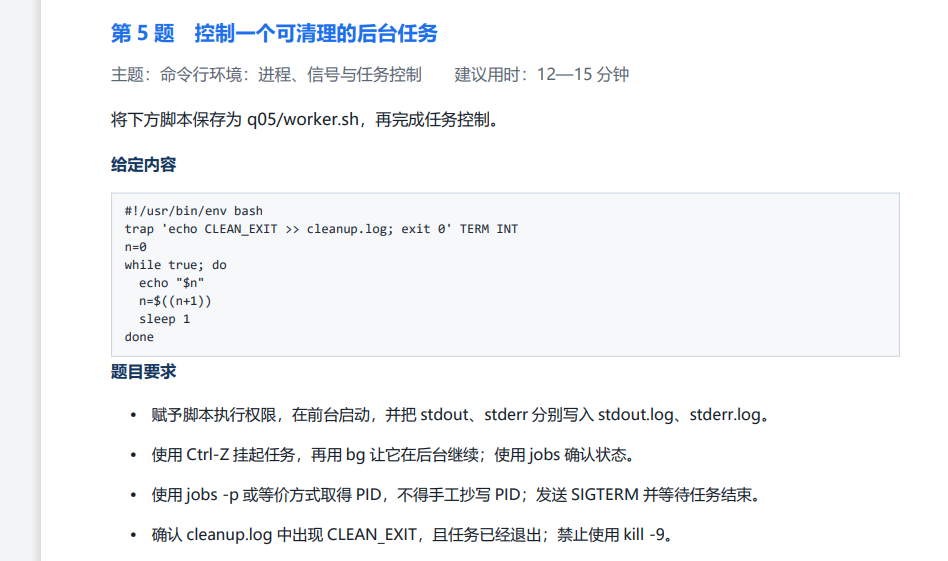
\includegraphics[width=0.9\textwidth]{q05_question.png}
    \caption{第 5 题题目要求}
    \label{fig:q05_question}
\end{figure}

给定脚本 worker.sh：

\begin{lstlisting}[language=bash, caption={q05/worker.sh（信号清理脚本）}]
#!/usr/bin/env bash
trap 'echo CLEAN_EXIT >> cleanup.log; exit 0' TERM INT
n=0
while true; do
  echo "$n"
  n=$((n+1))
  sleep 1
done
\end{lstlisting}

\begin{figure}[H]
    \centering
    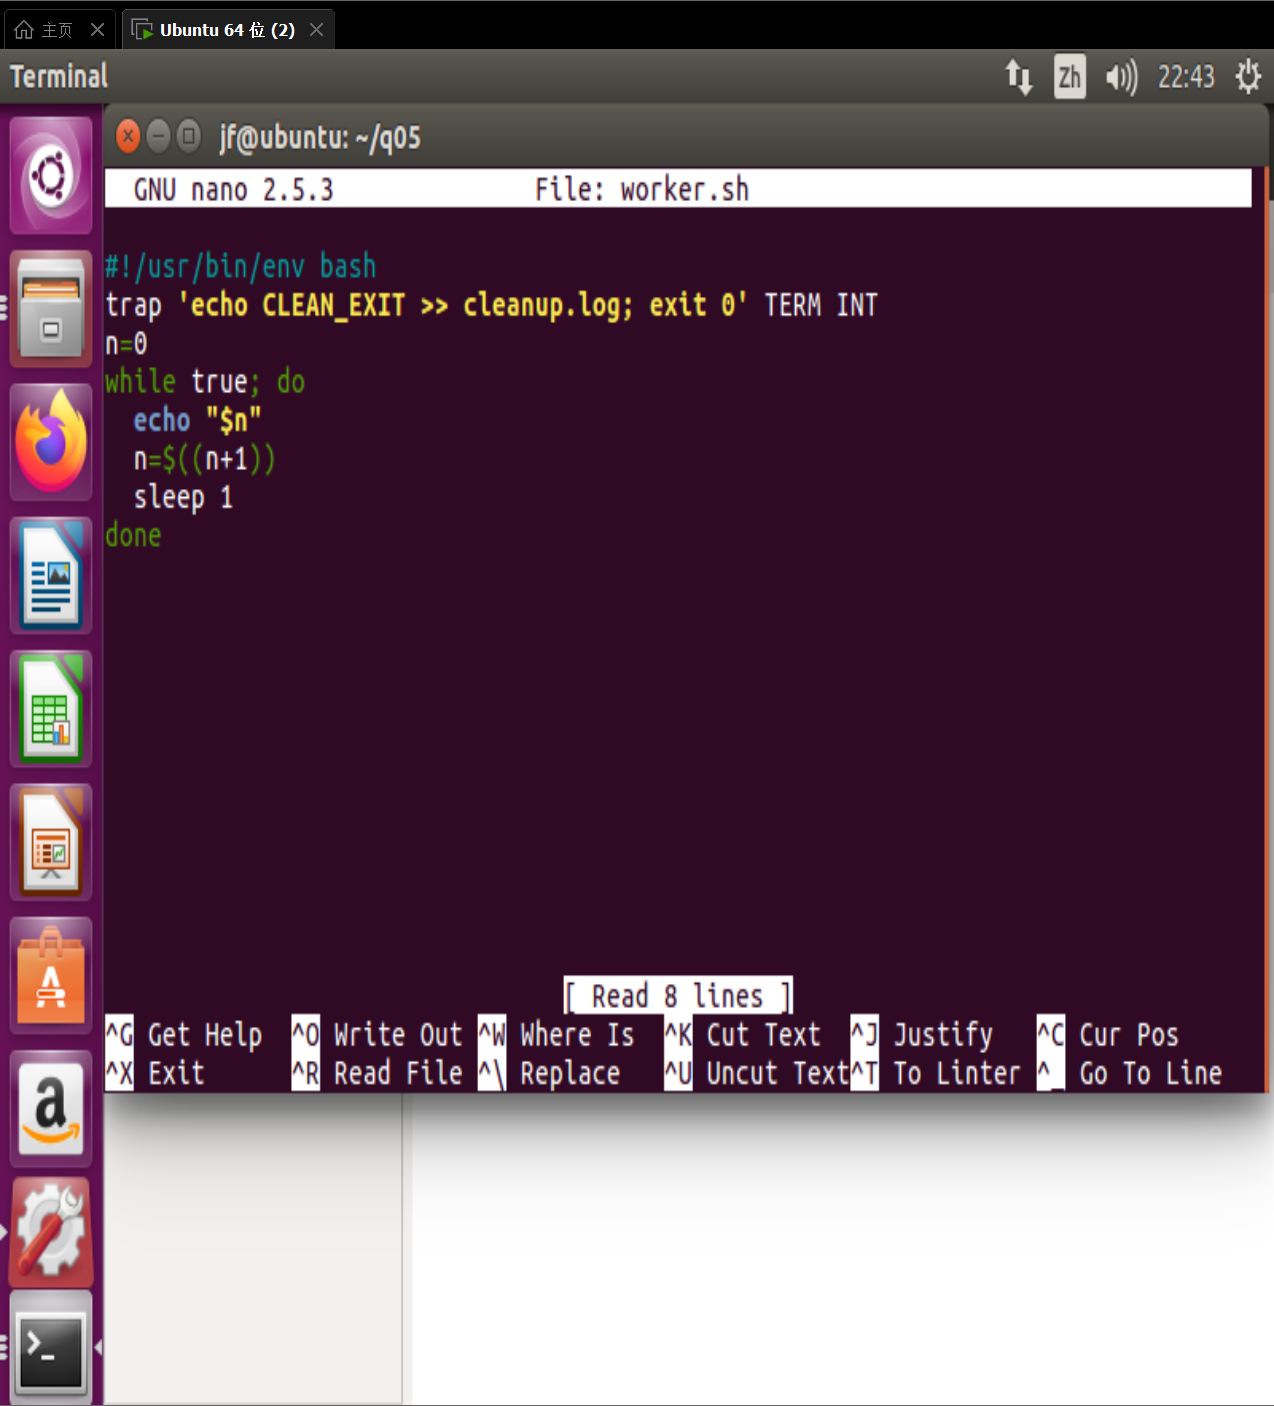
\includegraphics[width=0.9\textwidth]{q05_code_worker.png}
    \caption{nano 中编辑 worker.sh（trap 注册 TERM/INT 信号处理）}
    \label{fig:q05_code_worker}
\end{figure}

\subsubsection*{作答过程与关键代码}

在 q05 目录中创建 worker.sh（编辑时文件名曾误写成 wprker.sh，随后改正）：

\begin{lstlisting}[language=bash, caption={创建脚本并赋予执行权限}]
$ cd q05
$ nano worker.sh        # 注：实际操作中文件名一度误写为 wprker.sh，已改正
$ chmod +x worker.sh
\end{lstlisting}

\begin{figure}[H]
    \centering
    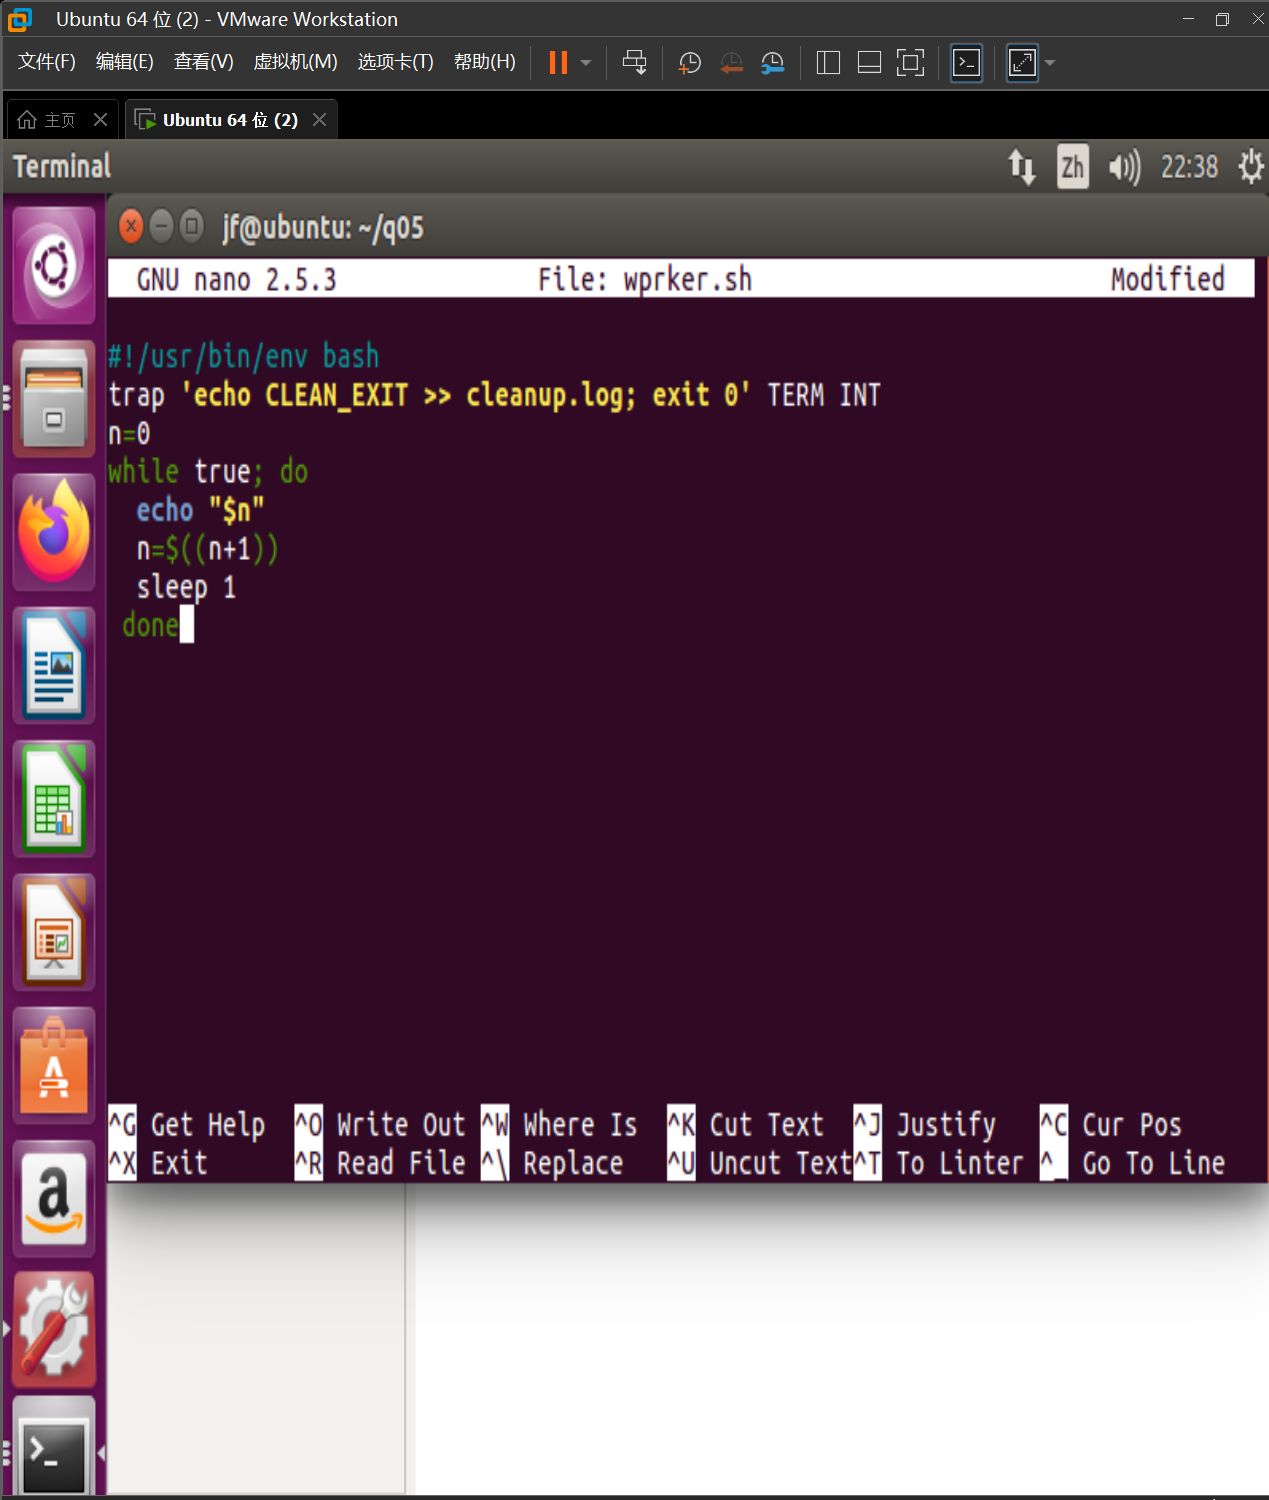
\includegraphics[width=0.9\textwidth]{q05_code_mistyped.png}
    \caption{文件名误写为 wprker.sh 的编辑界面（后已改正为 worker.sh）}
    \label{fig:q05_code_mistyped}
\end{figure}

按题目要求完成任务控制全过程：

\begin{lstlisting}[language=bash, caption={前台启动、挂起、后台运行、取 PID、发信号、验证}]
$ ./worker.sh > stdout.log 2> stderr.log   # 前台启动并重定向 stdout/stderr
^Z                                         # Ctrl-Z 挂起
[1]+  Stopped  ./worker.sh > stdout.log 2> stderr.log
$ bg                                       # 转后台继续
[1]+  ./worker.sh > stdout.log 2> stderr.log &
$ jobs                                     # 确认任务状态
[1]+  Running  ./worker.sh > stdout.log 2> stderr.log &
$ PID=$(jobs -p)                           # 动态取得 PID（不手工抄写）
$ echo "PID=$PID"                          # PID=16293
$ kill -TERM $PID                          # 发送 SIGTERM，触发 trap
$ wait $PID                                # 等待任务结束
[1]+  Done  ./worker.sh > stdout.log 2> stderr.log
$ cat cleanup.log                          # 验证清理日志
CLEAN_EXIT
\end{lstlisting}

\begin{figure}[H]
    \centering
    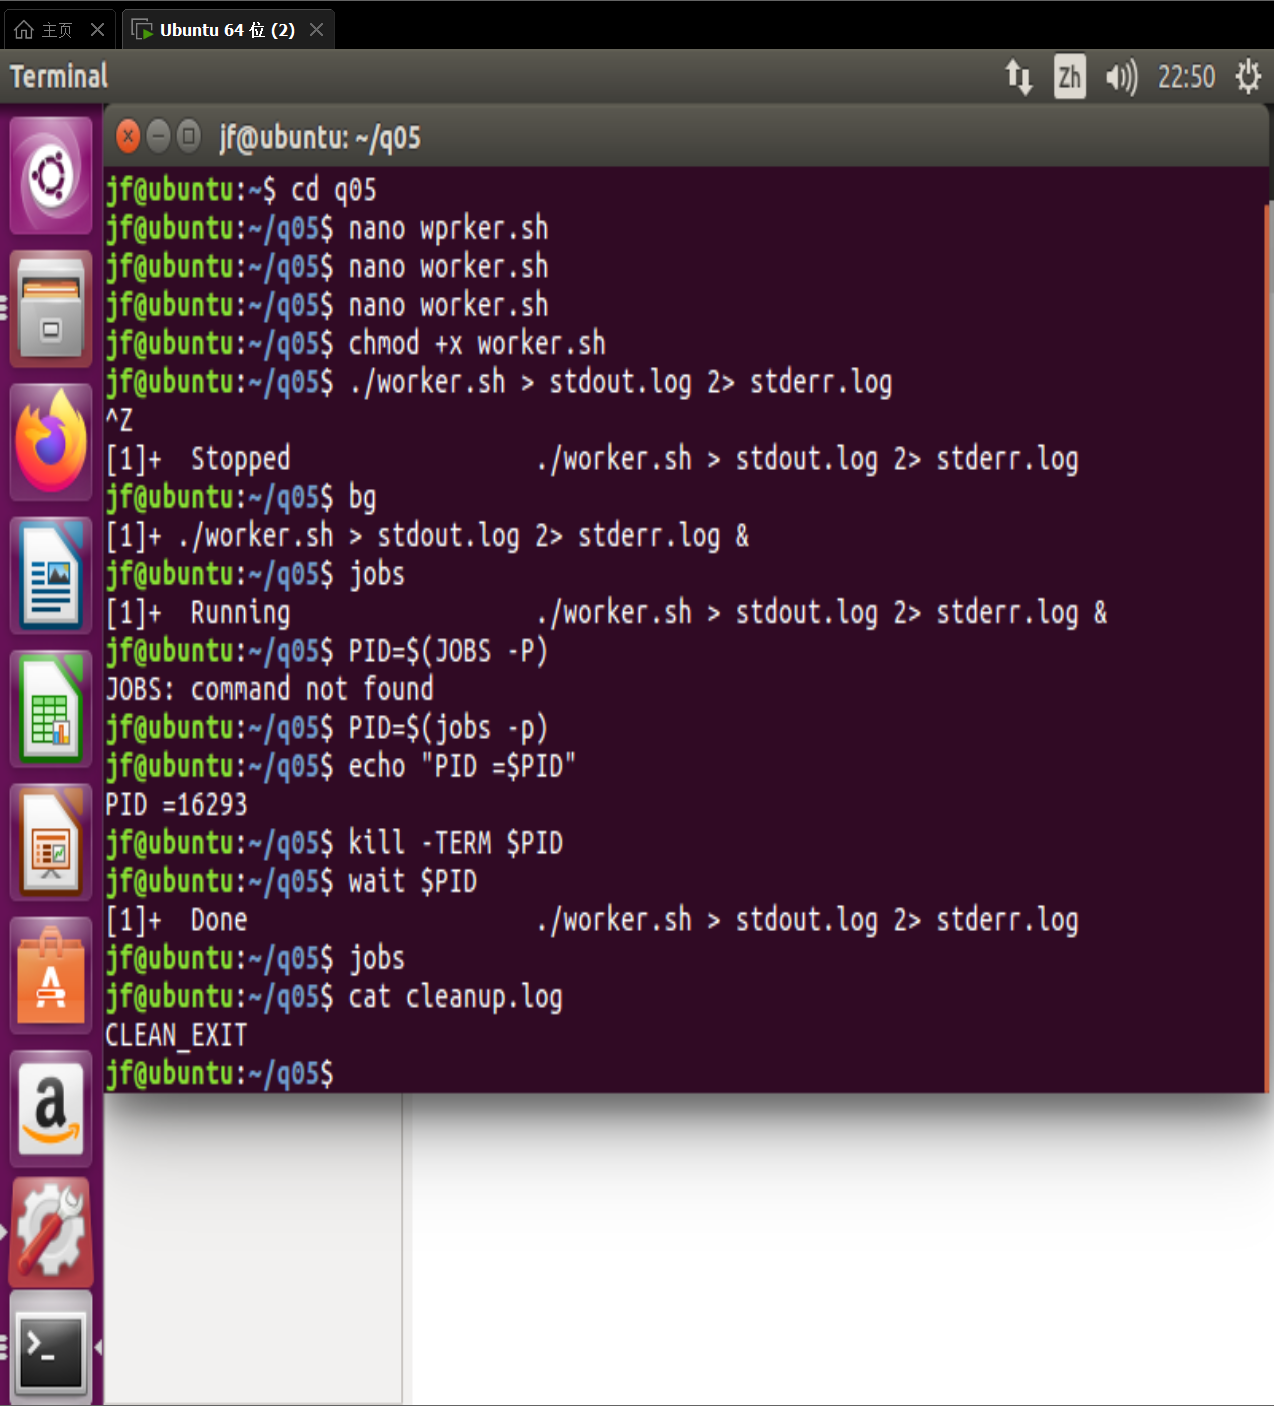
\includegraphics[width=0.9\textwidth]{q05_run.png}
    \caption{任务控制完整执行过程（最终 cleanup.log 输出 CLEAN\_EXIT）}
    \label{fig:q05_run}
\end{figure}

\subsubsection*{运行结果与小结}

worker.sh 通过 \texttt{trap} 注册了 TERM 和 INT 两个信号的处理函数：收到信号后把 CLEAN\_EXIT 写入 cleanup.log 并以状态 0 退出，因此只需发送 SIGTERM（kill -TERM）就能让程序"优雅退出"，无需 kill -9。操作中先用 Ctrl-Z 挂起、bg 转后台、jobs 确认状态；再用 jobs -p 动态取得 PID（避免手工抄写）；kill -TERM 触发 trap 后，wait 等待任务结束；最终 cat cleanup.log 看到 CLEAN\_EXIT，验证任务已按预期清理退出。

% ==================== 第 6 题 ====================
\subsection{第 6 题：语义重构与本地开发反馈}

\textbf{题目}：在 q06 中按照给定代码创建三个 Python 文件，并使用编辑器语言服务器完成一次语义重构：
(1) 在已配置好 Python、pytest 和 ruff 的课程环境中打开 q06，并启用 Python 语言服务器；
(2) 分别演示跳转到定义和查找引用；
(3) 使用"重命名符号"把 total\_price 改为 calculate\_total，保证定义和所有代码引用同步改变；
(4) 在 app.py 中临时加入未使用的 import os，用 ruff 发现并删除；最后运行 ruff 和 pytest 并保证通过。

\begin{figure}[H]
    \centering
    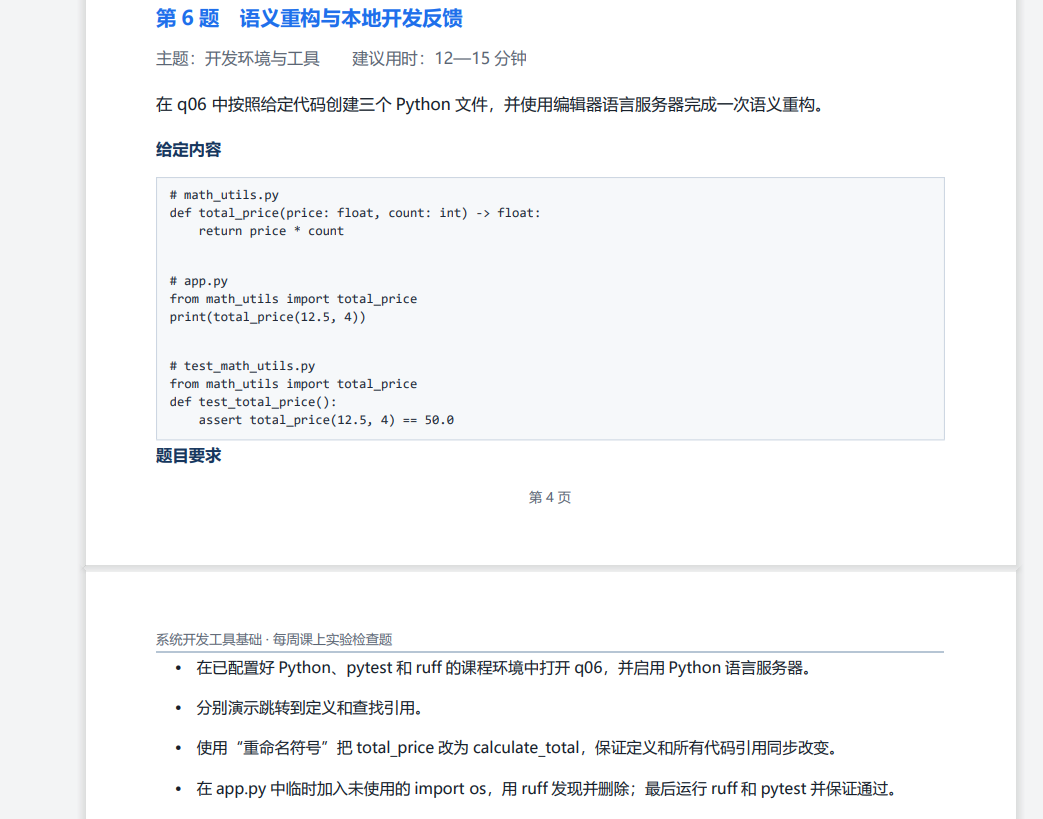
\includegraphics[width=0.9\textwidth]{q06_question.png}
    \caption{第 6 题题目要求}
    \label{fig:q06_question}
\end{figure}

给定三个文件：

\begin{lstlisting}[language=Python, caption={math\_utils.py / app.py / test\_math\_utils.py}]
# math_utils.py
def total_price(price: float, count: int) -> float:
    return price * count

# app.py
from math_utils import total_price
print(total_price(12.5, 4))

# test_math_utils.py
from math_utils import total_price
def test_total_price():
    assert total_price(12.5, 4) == 50.0
\end{lstlisting}

\subsubsection*{作答过程与关键代码}

先用 nano 创建三个文件：

\begin{figure}[H]
    \centering
    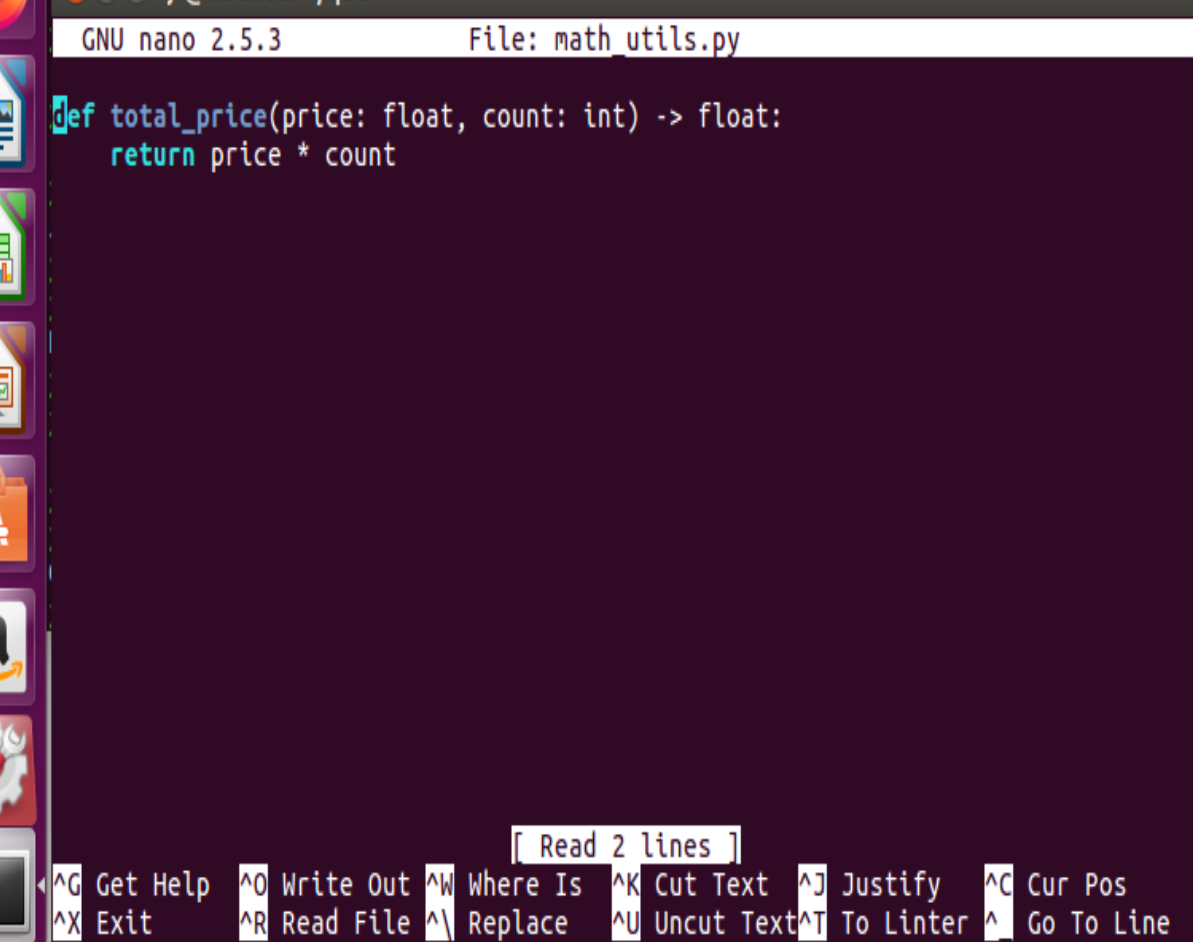
\includegraphics[width=0.9\textwidth]{q06_code_math_utils.png}
    \caption{nano 中编辑 math\_utils.py}
    \label{fig:q06_code_math_utils}
\end{figure}

\begin{figure}[H]
    \centering
    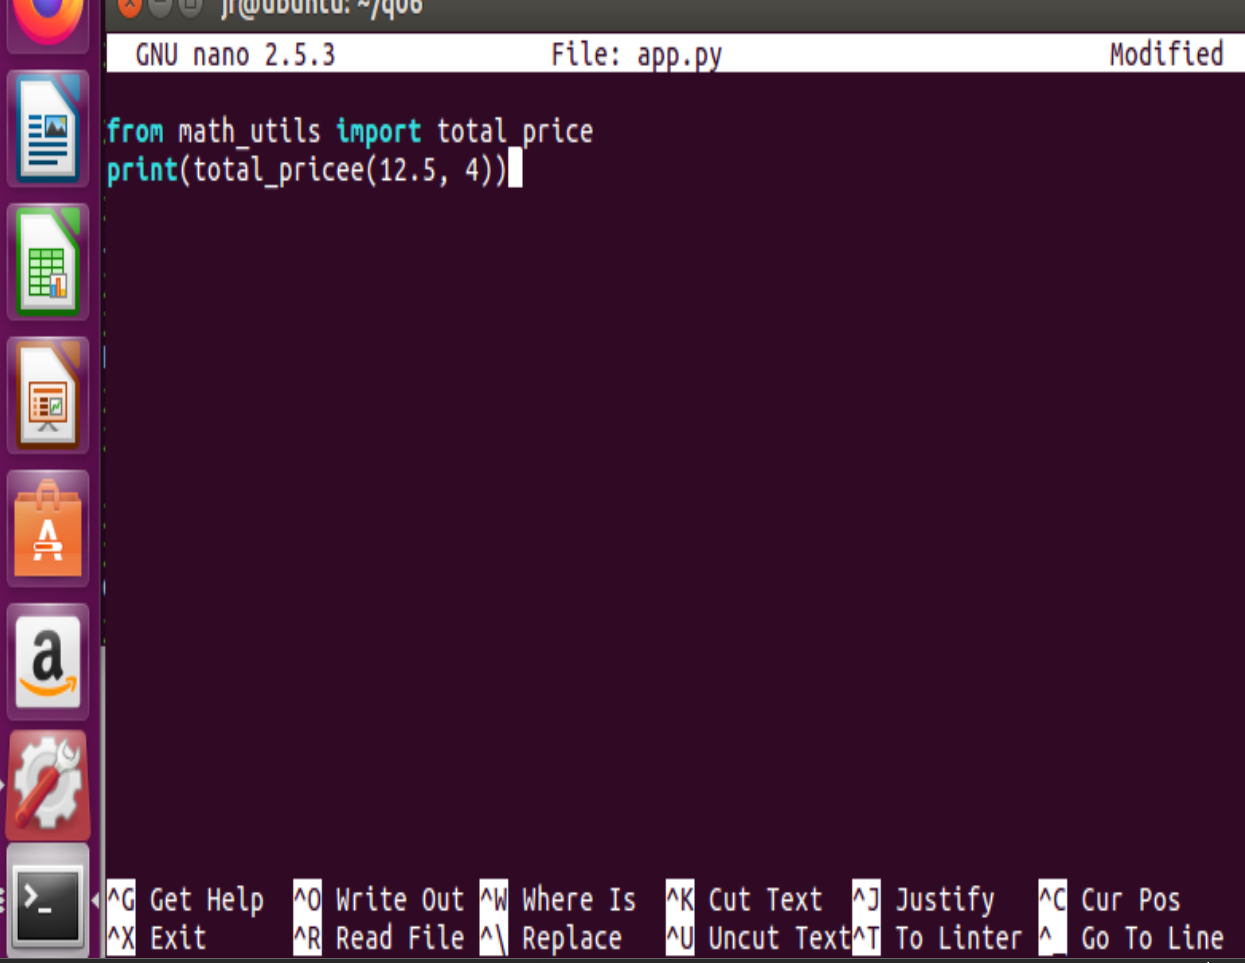
\includegraphics[width=0.9\textwidth]{q06_code_app.png}
    \caption{nano 中编辑 app.py（曾将 total\_price 误写为 total\_pricee，已纠正）}
    \label{fig:q06_code_app}
\end{figure}

\begin{figure}[H]
    \centering
    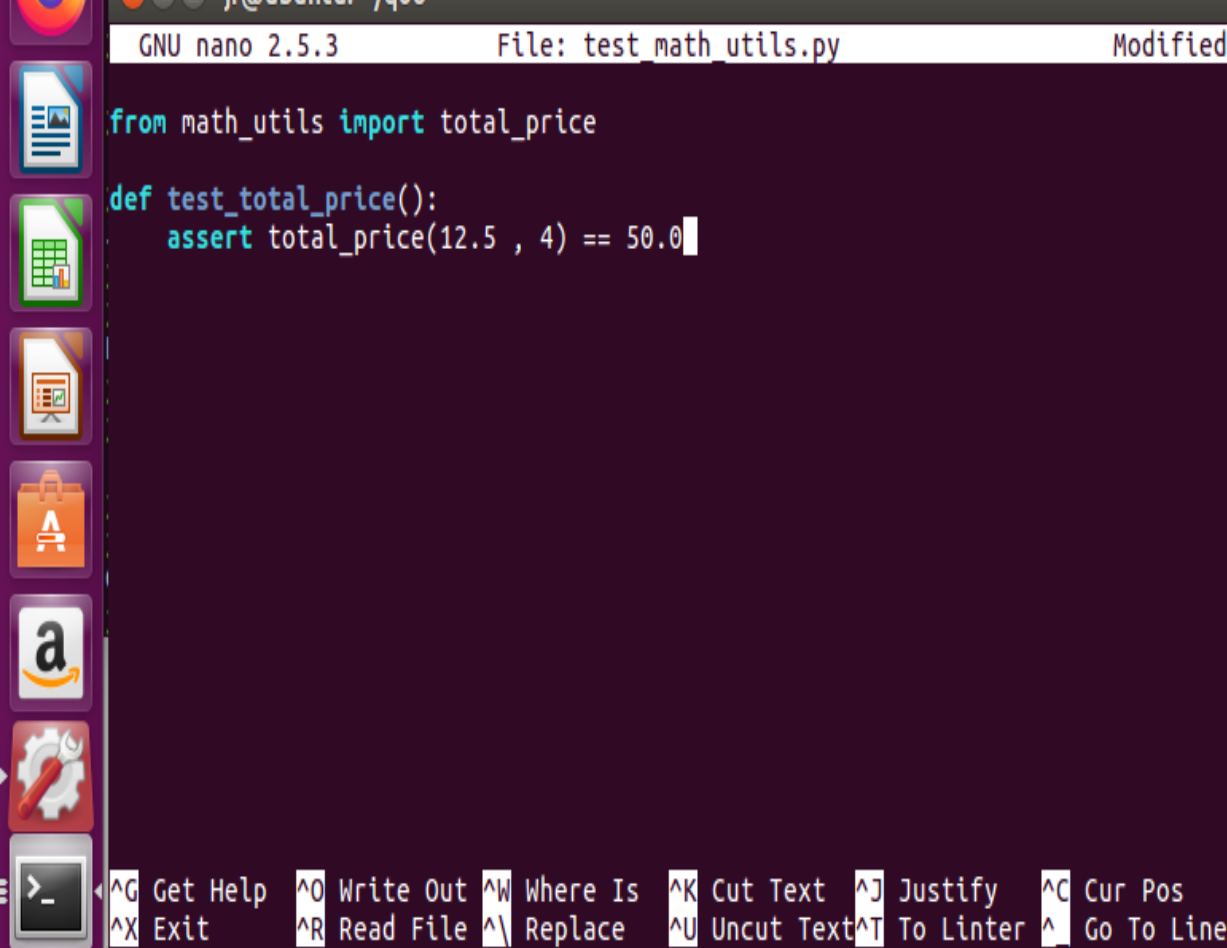
\includegraphics[width=0.9\textwidth]{q06_code_test.png}
    \caption{nano 中编辑 test\_math\_utils.py}
    \label{fig:q06_code_test}
\end{figure}

用 VS Code 打开 q06 文件夹，启用 Python 语言服务器：

\begin{figure}[H]
    \centering
    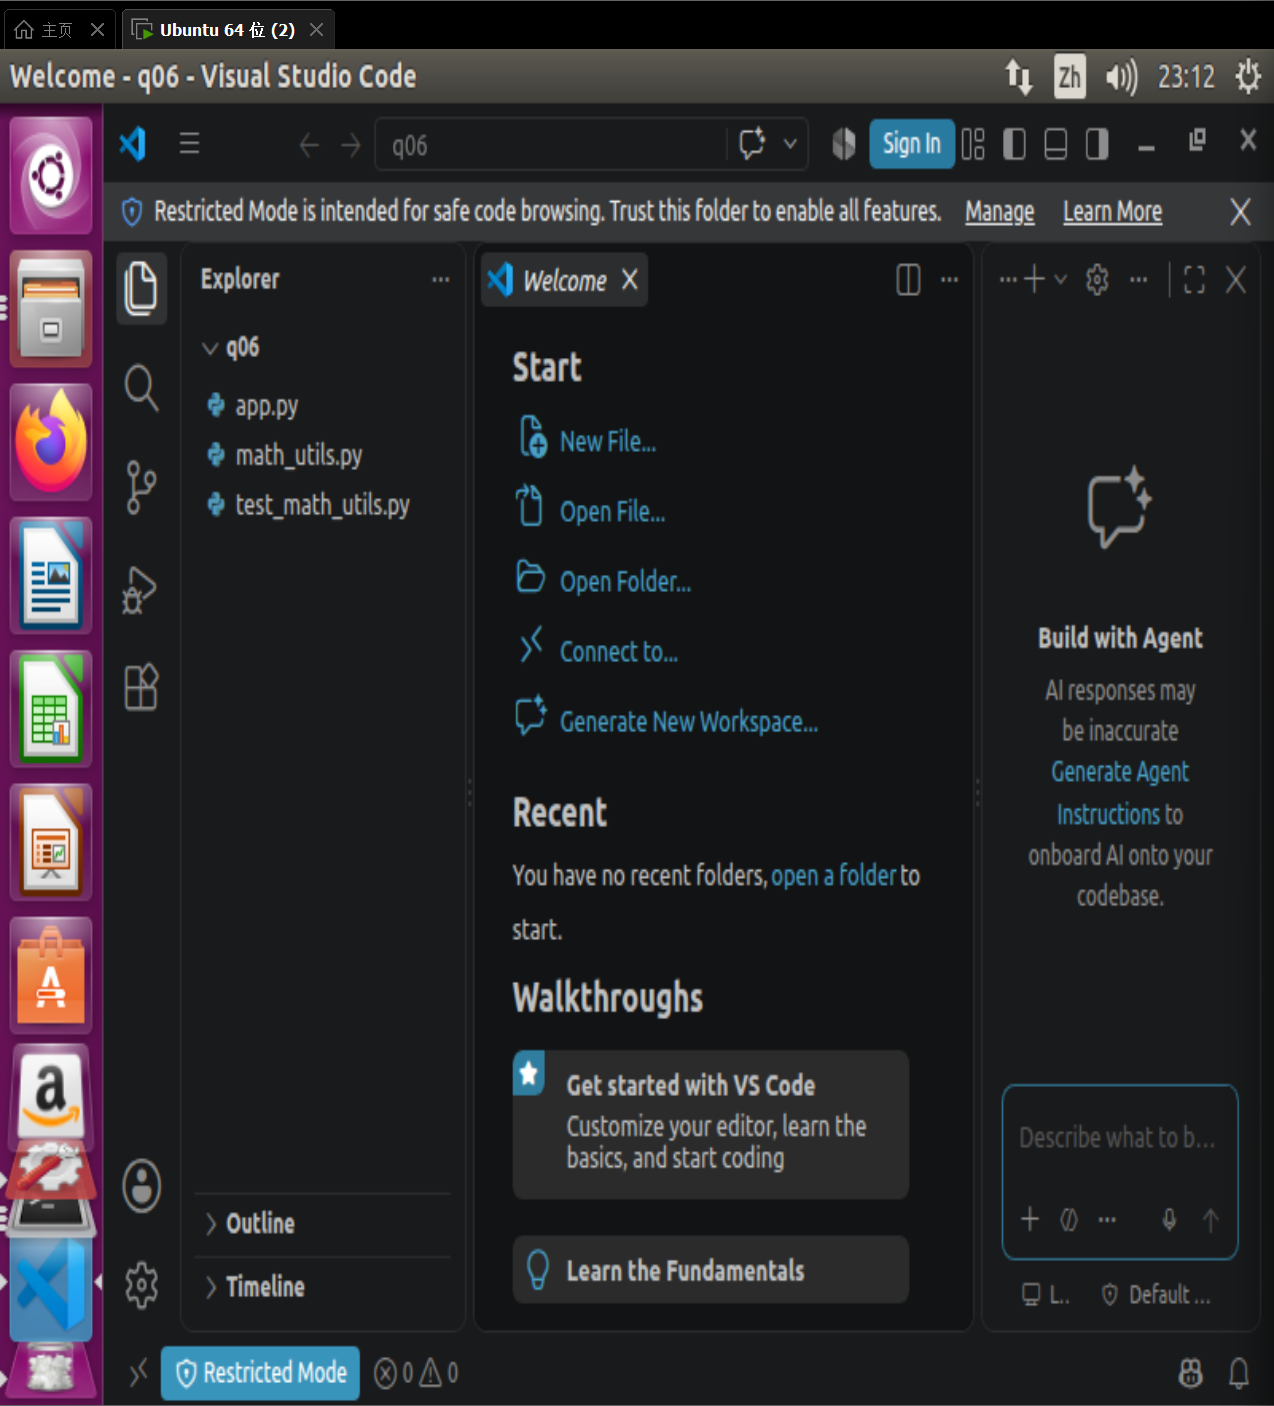
\includegraphics[width=0.9\textwidth]{q06_vscode_open.png}
    \caption{VS Code 打开 q06 工作区（三个 Python 文件）}
    \label{fig:q06_vscode_open}
\end{figure}

演示"跳转到定义"——从 app.py 的调用处跳到 math\_utils.py 中 total\_price 的定义：

\begin{figure}[H]
    \centering
    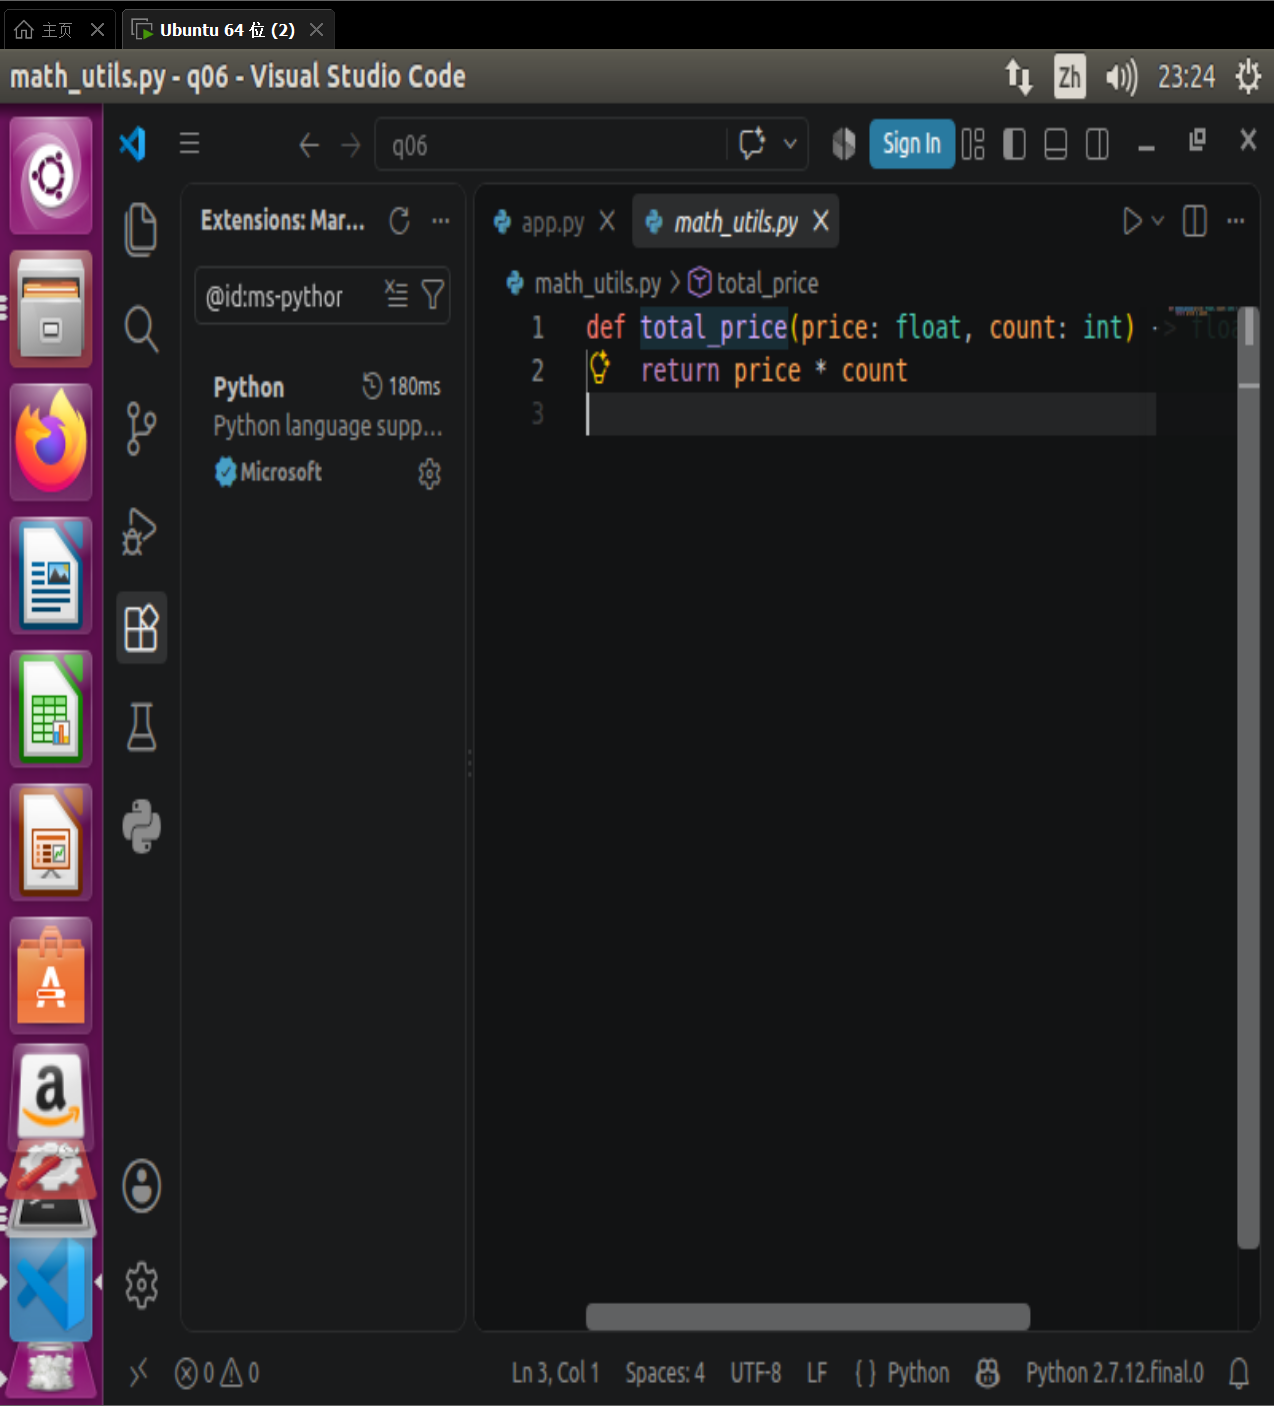
\includegraphics[width=0.9\textwidth]{q06_goto_def.png}
    \caption{跳转到定义（math\_utils.py 中的 total\_price）}
    \label{fig:q06_goto_def}
\end{figure}

演示"查找引用"——total\_price 在多个文件中被引用：

\begin{figure}[H]
    \centering
    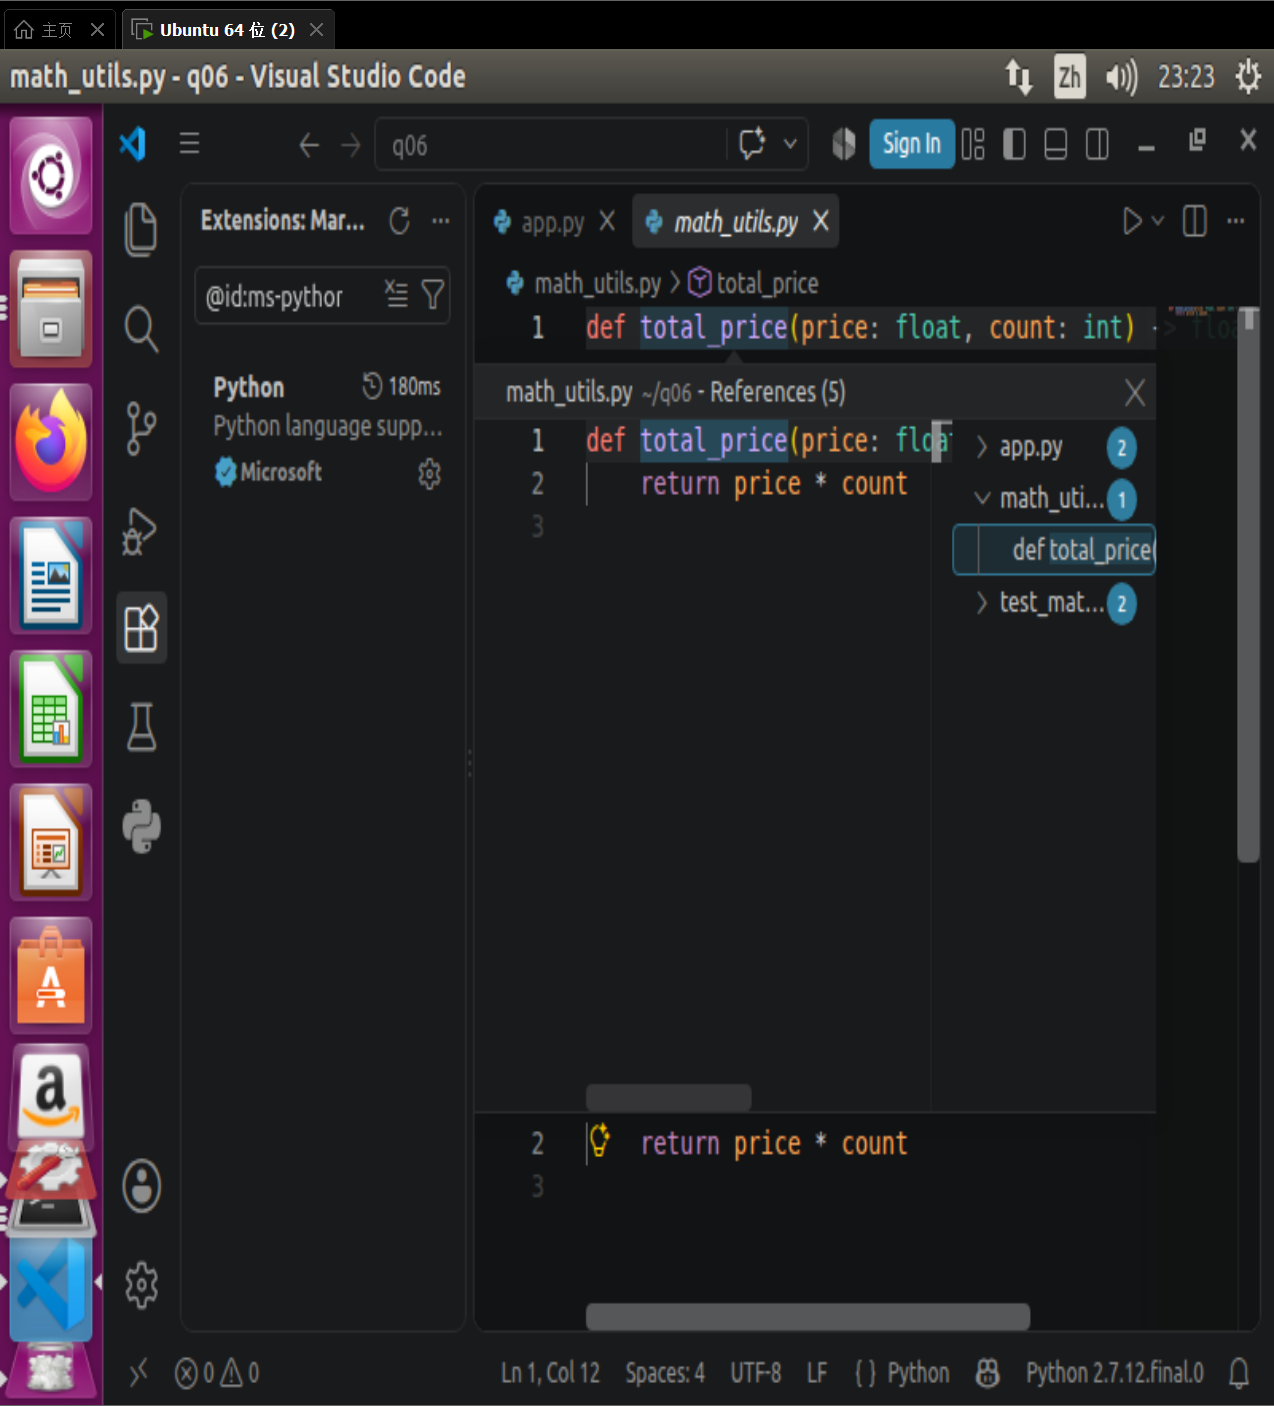
\includegraphics[width=0.9\textwidth]{q06_references.png}
    \caption{查找引用（References: 5）}
    \label{fig:q06_references}
\end{figure}

使用"重命名符号"把 total\_price 改为 calculate\_total，定义与所有引用同步更新：

\begin{figure}[H]
    \centering
    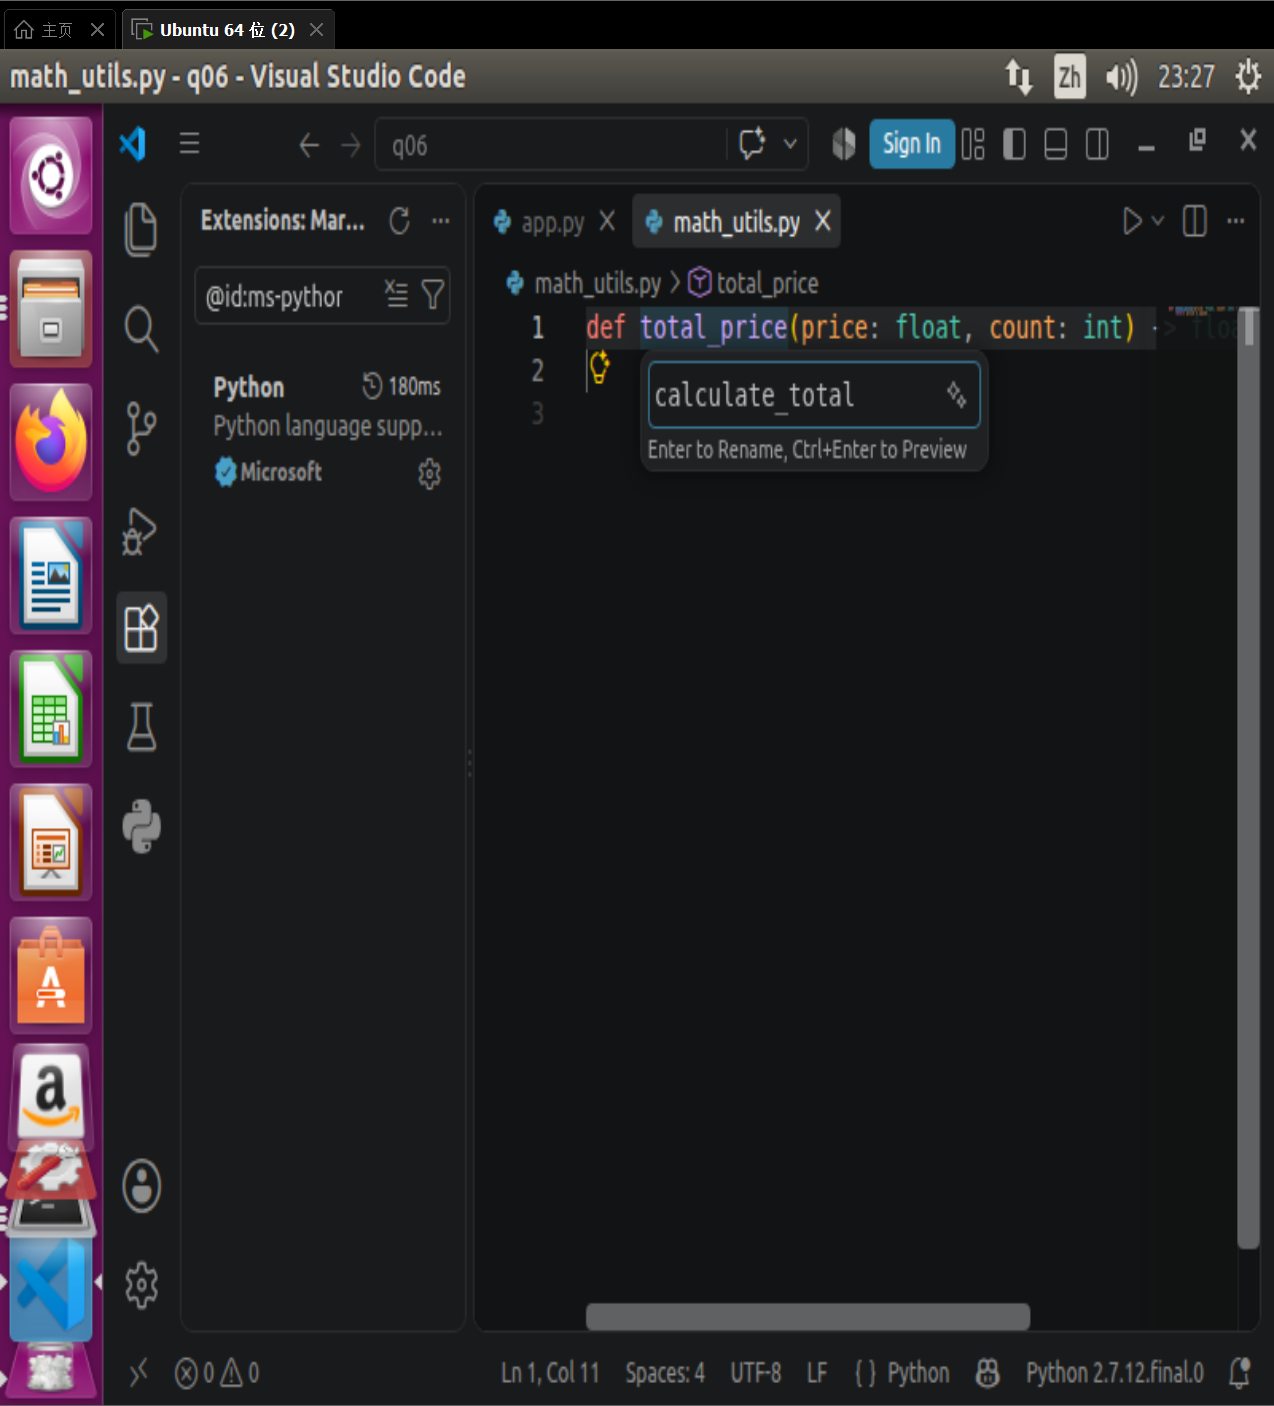
\includegraphics[width=0.9\textwidth]{q06_rename_done.png}
    \caption{重命名符号为 calculate\_total（Enter 确认后同步所有引用）}
    \label{fig:q06_rename_done}
\end{figure}

重命名后，在 app.py 中临时加入未使用的 import os：

\begin{figure}[H]
    \centering
    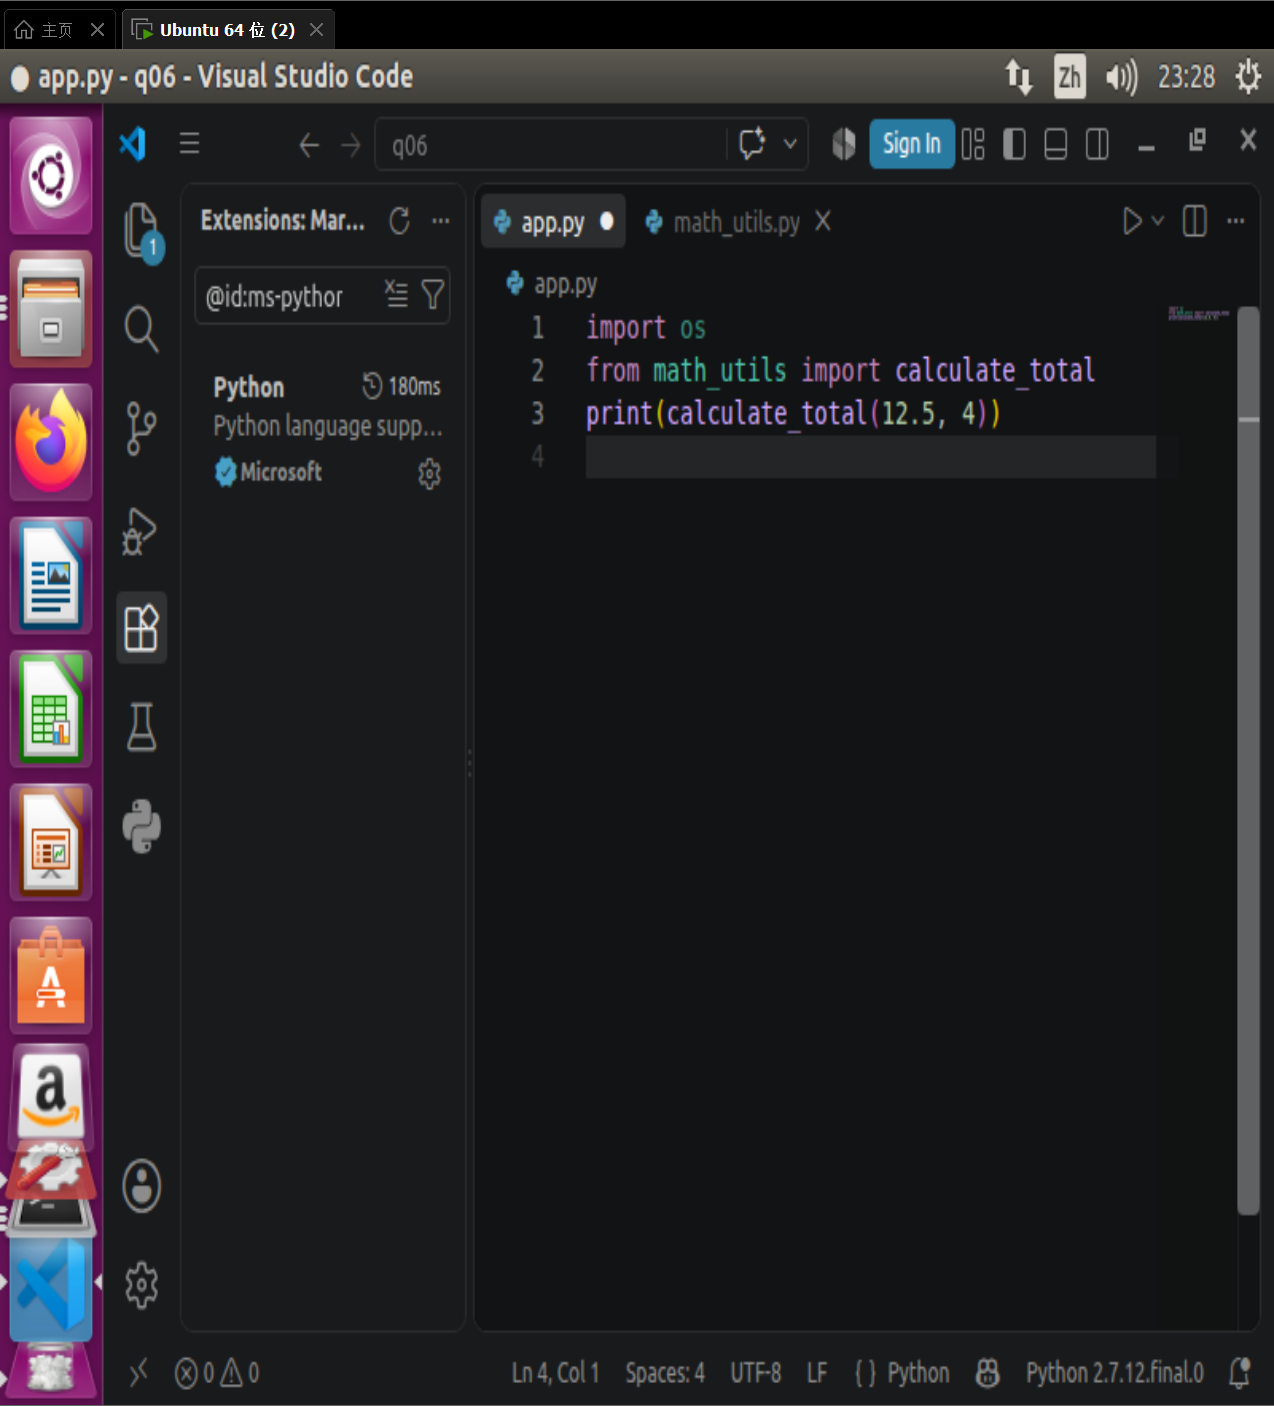
\includegraphics[width=0.9\textwidth]{q06_app_import_os.png}
    \caption{app.py 中加入未使用的 import os（calculate\_total 已同步）}
    \label{fig:q06_app_import_os}
\end{figure}

环境说明：系统自带的 Python 为 3.5.2 且未安装 ruff、pip，无法直接使用，因此安装 Miniconda（Python 3.11.7）并安装 ruff、pytest：

\begin{figure}[H]
    \centering
    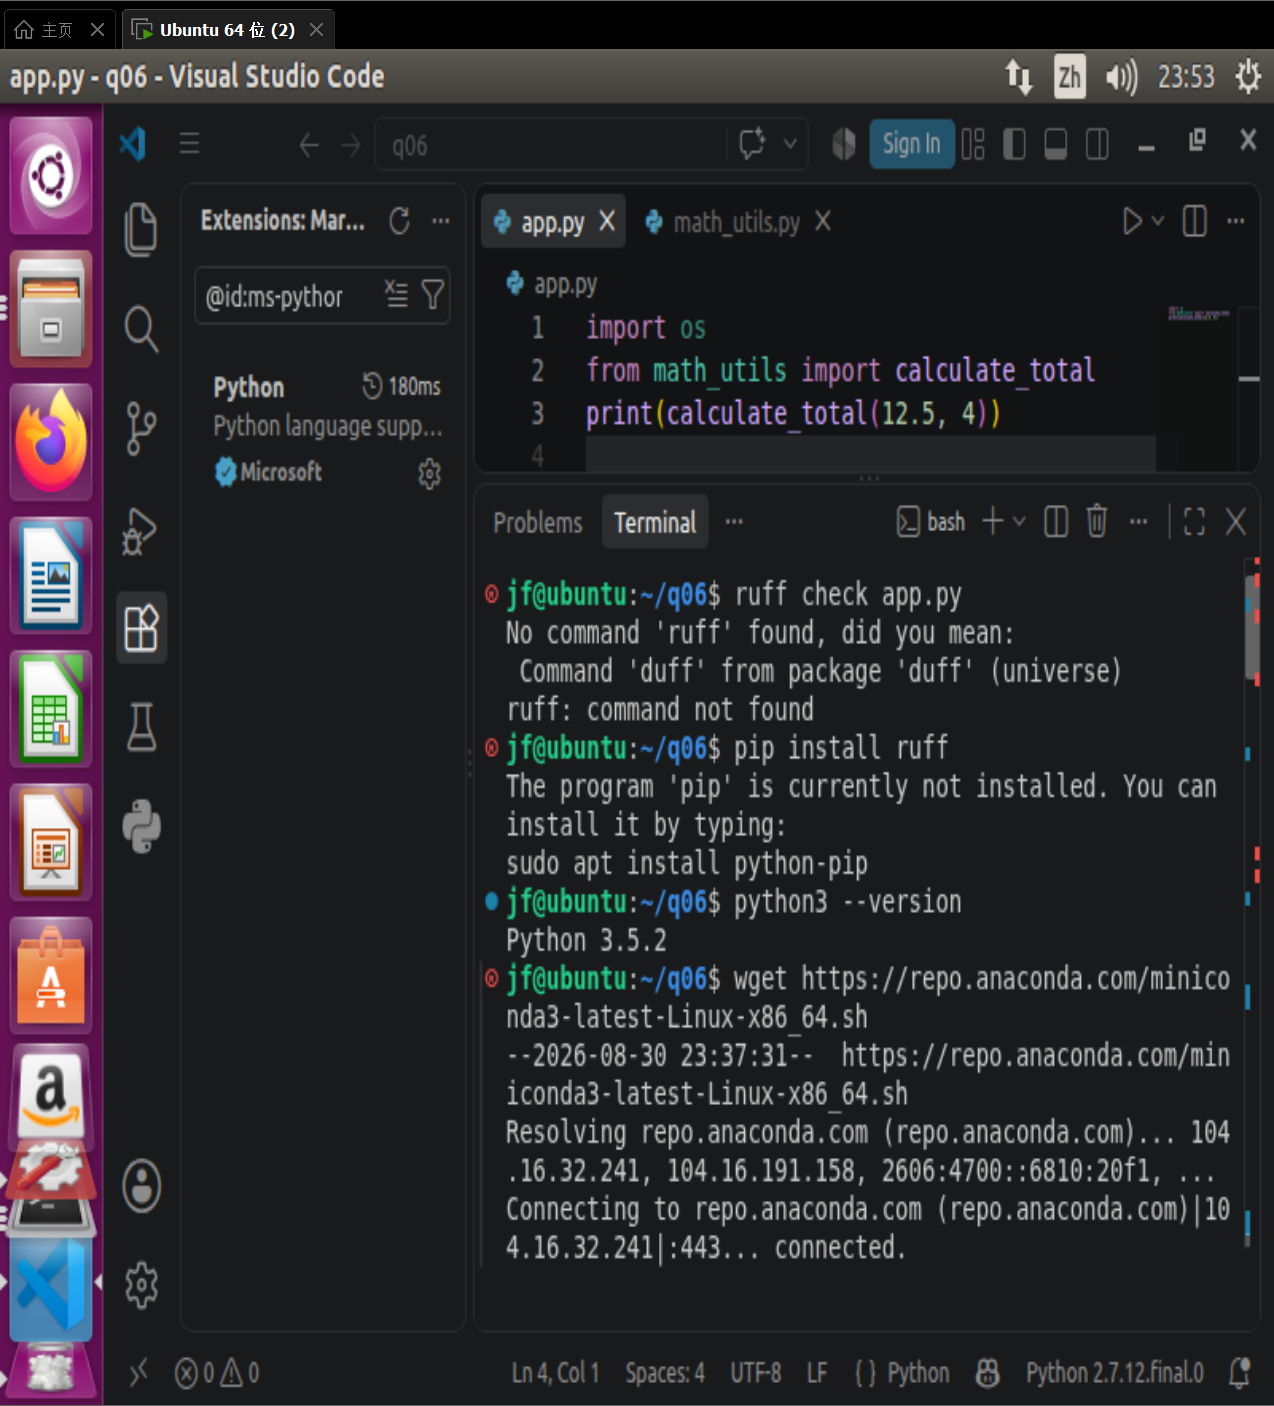
\includegraphics[width=0.9\textwidth]{q06_env_problem.png}
    \caption{系统 Python 3.5.2 过老、ruff/pip 缺失，改用 Miniconda}
    \label{fig:q06_env_problem}
\end{figure}

\begin{figure}[H]
    \centering
    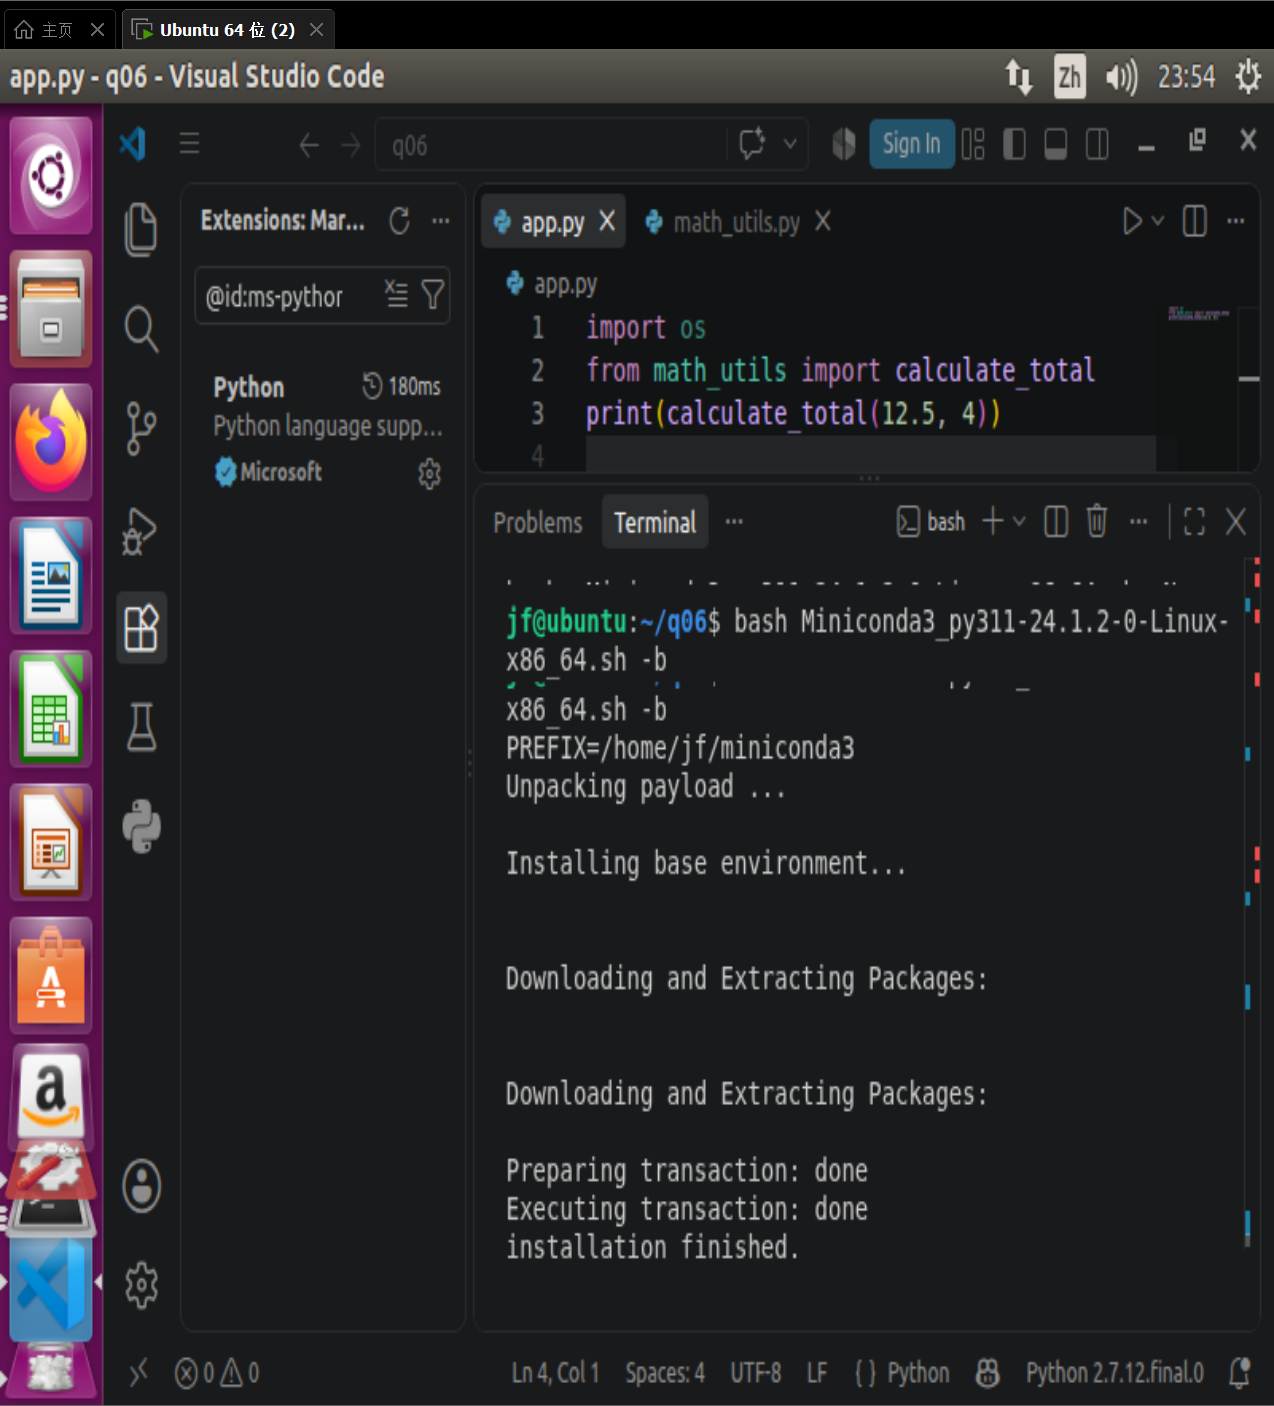
\includegraphics[width=0.9\textwidth]{q06_conda_install.png}
    \caption{Miniconda 安装完成}
    \label{fig:q06_conda_install}
\end{figure}

\begin{figure}[H]
    \centering
    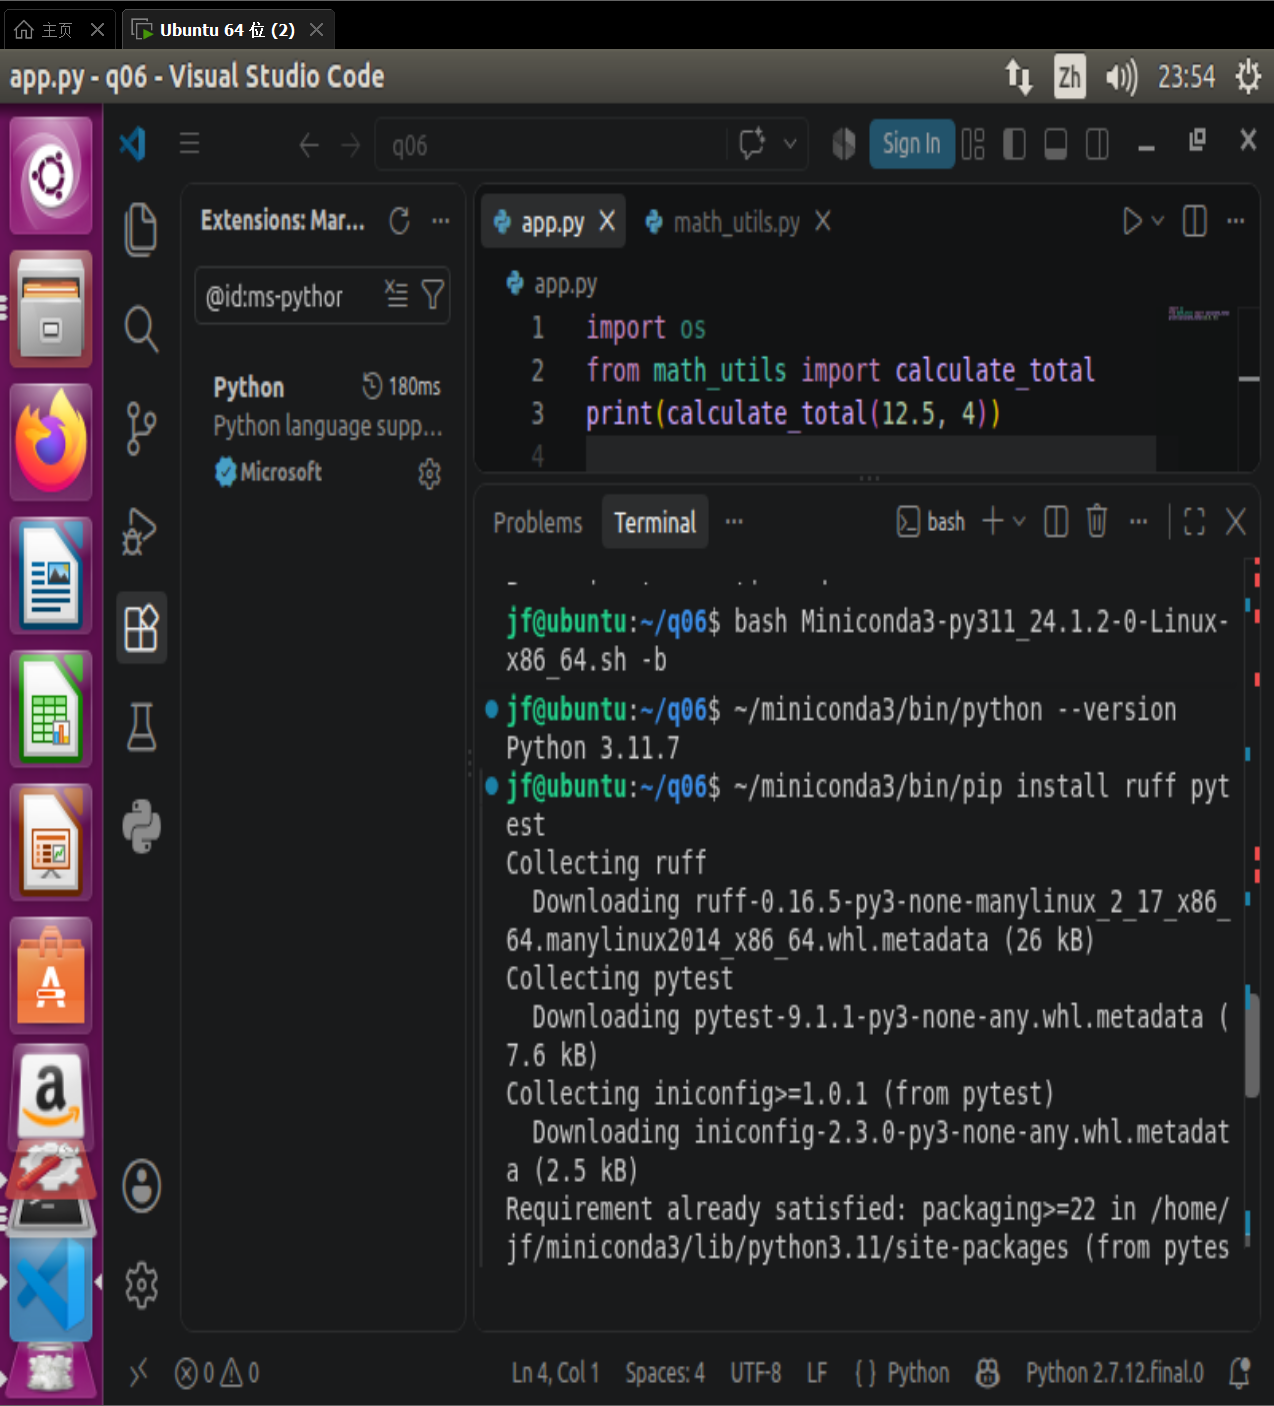
\includegraphics[width=0.9\textwidth]{q06_py311_pip.png}
    \caption{Python 3.11.7 就绪，pip install ruff pytest}
    \label{fig:q06_py311_pip}
\end{figure}

运行 ruff 检查 app.py，发现未使用的 import os：

\begin{figure}[H]
    \centering
    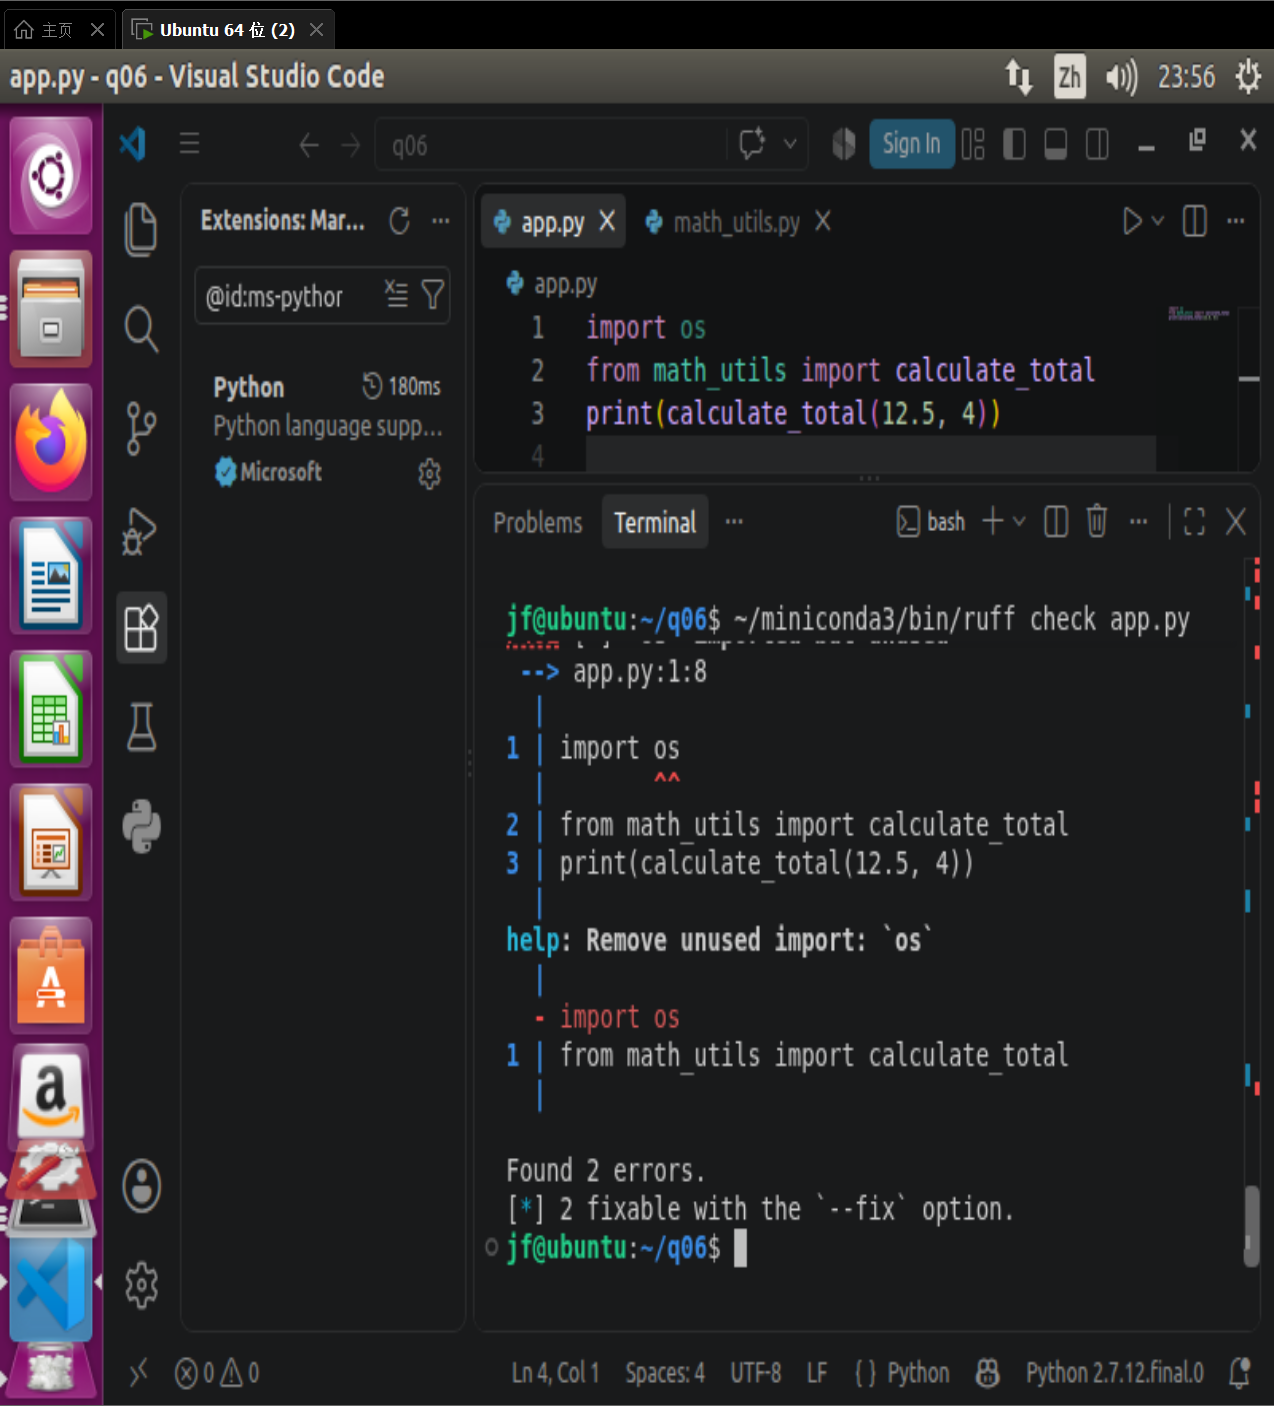
\includegraphics[width=0.9\textwidth]{q06_ruff_os.png}
    \caption{ruff check app.py：提示 Remove unused import: os}
    \label{fig:q06_ruff_os}
\end{figure}

使用 ruff --fix 自动删除未使用的导入：

\begin{figure}[H]
    \centering
    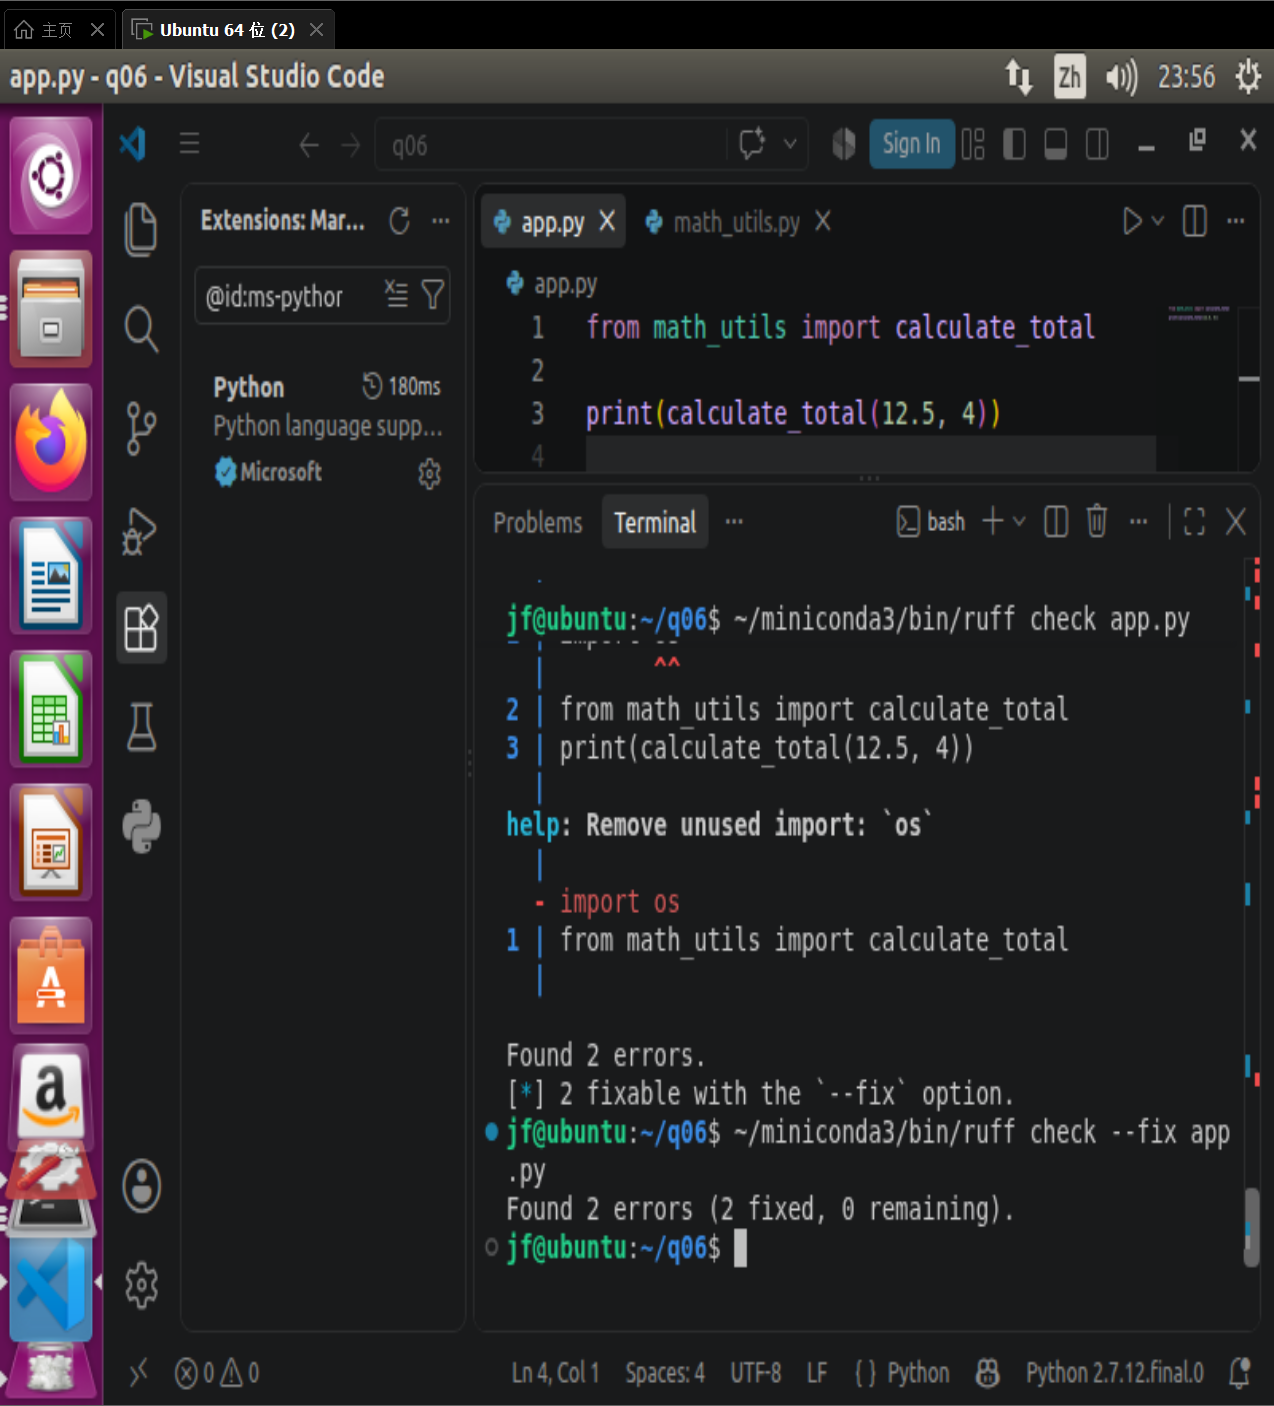
\includegraphics[width=0.9\textwidth]{q06_ruff_fix.png}
    \caption{ruff check --fix：2 fixed，os 导入被移除}
    \label{fig:q06_ruff_fix}
\end{figure}

再次检查通过，并运行 pytest：

\begin{figure}[H]
    \centering
    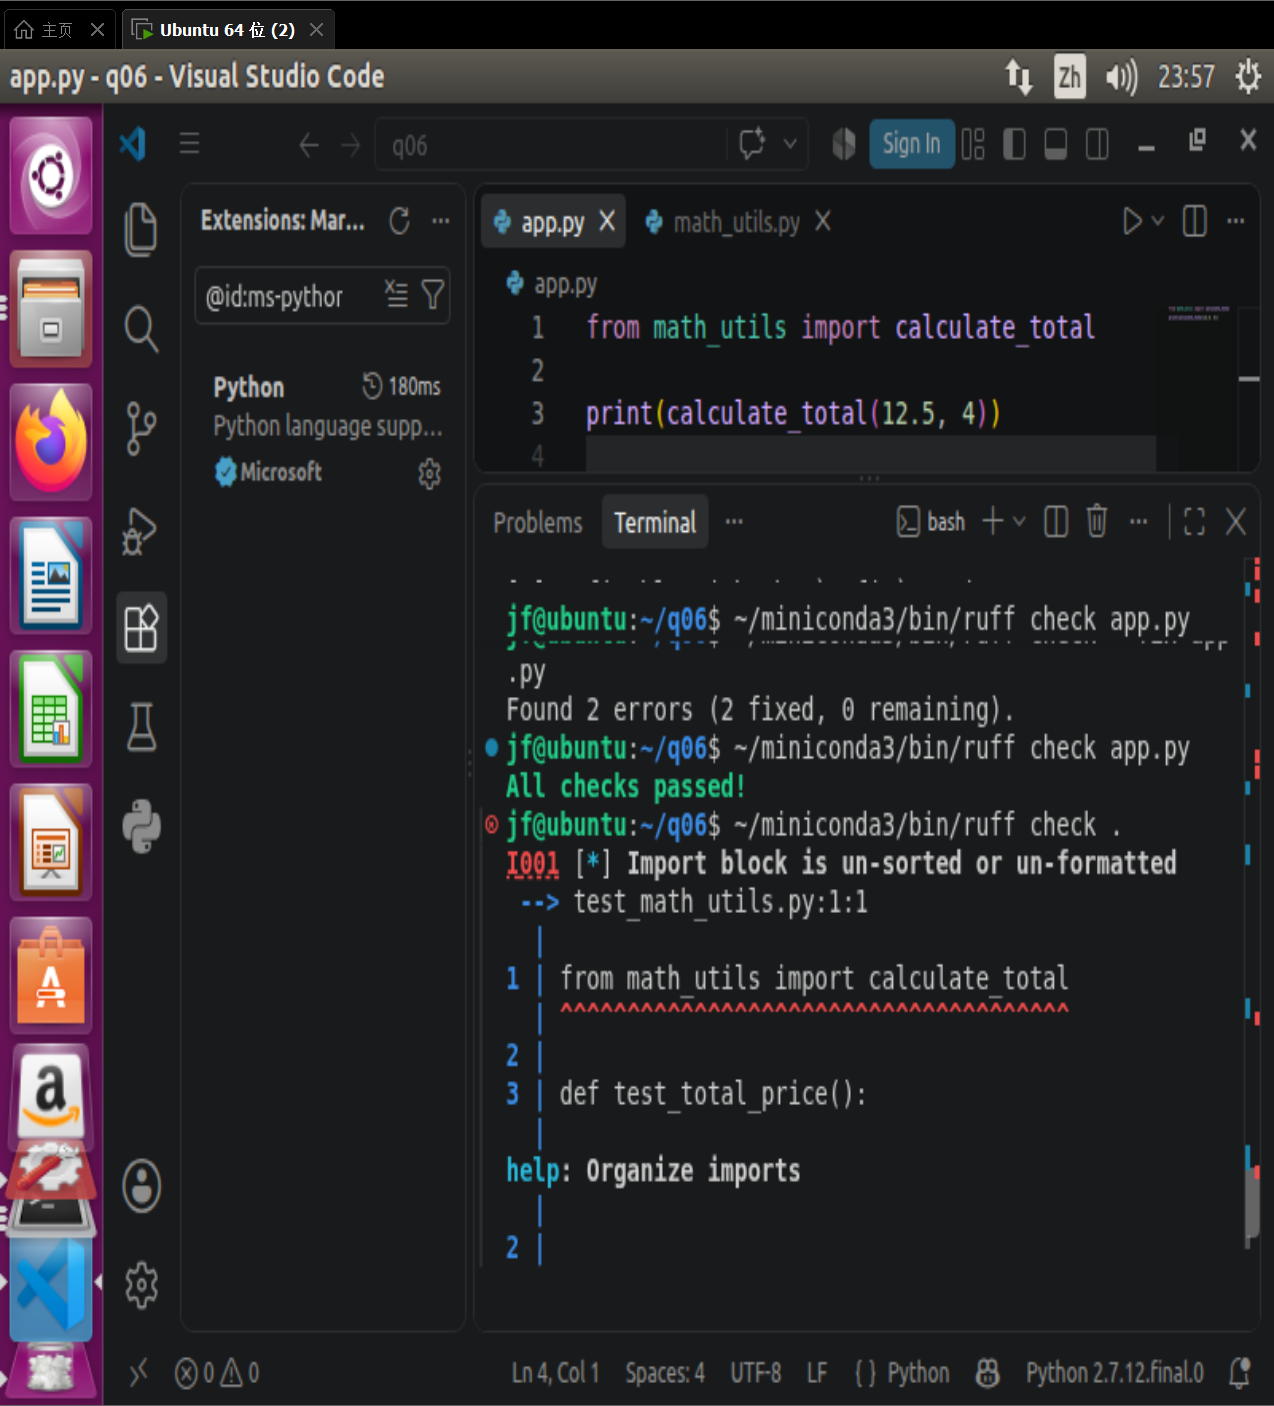
\includegraphics[width=0.9\textwidth]{q06_ruff_pass.png}
    \caption{ruff check 全部通过（All checks passed）}
    \label{fig:q06_ruff_pass}
\end{figure}

\begin{figure}[H]
    \centering
    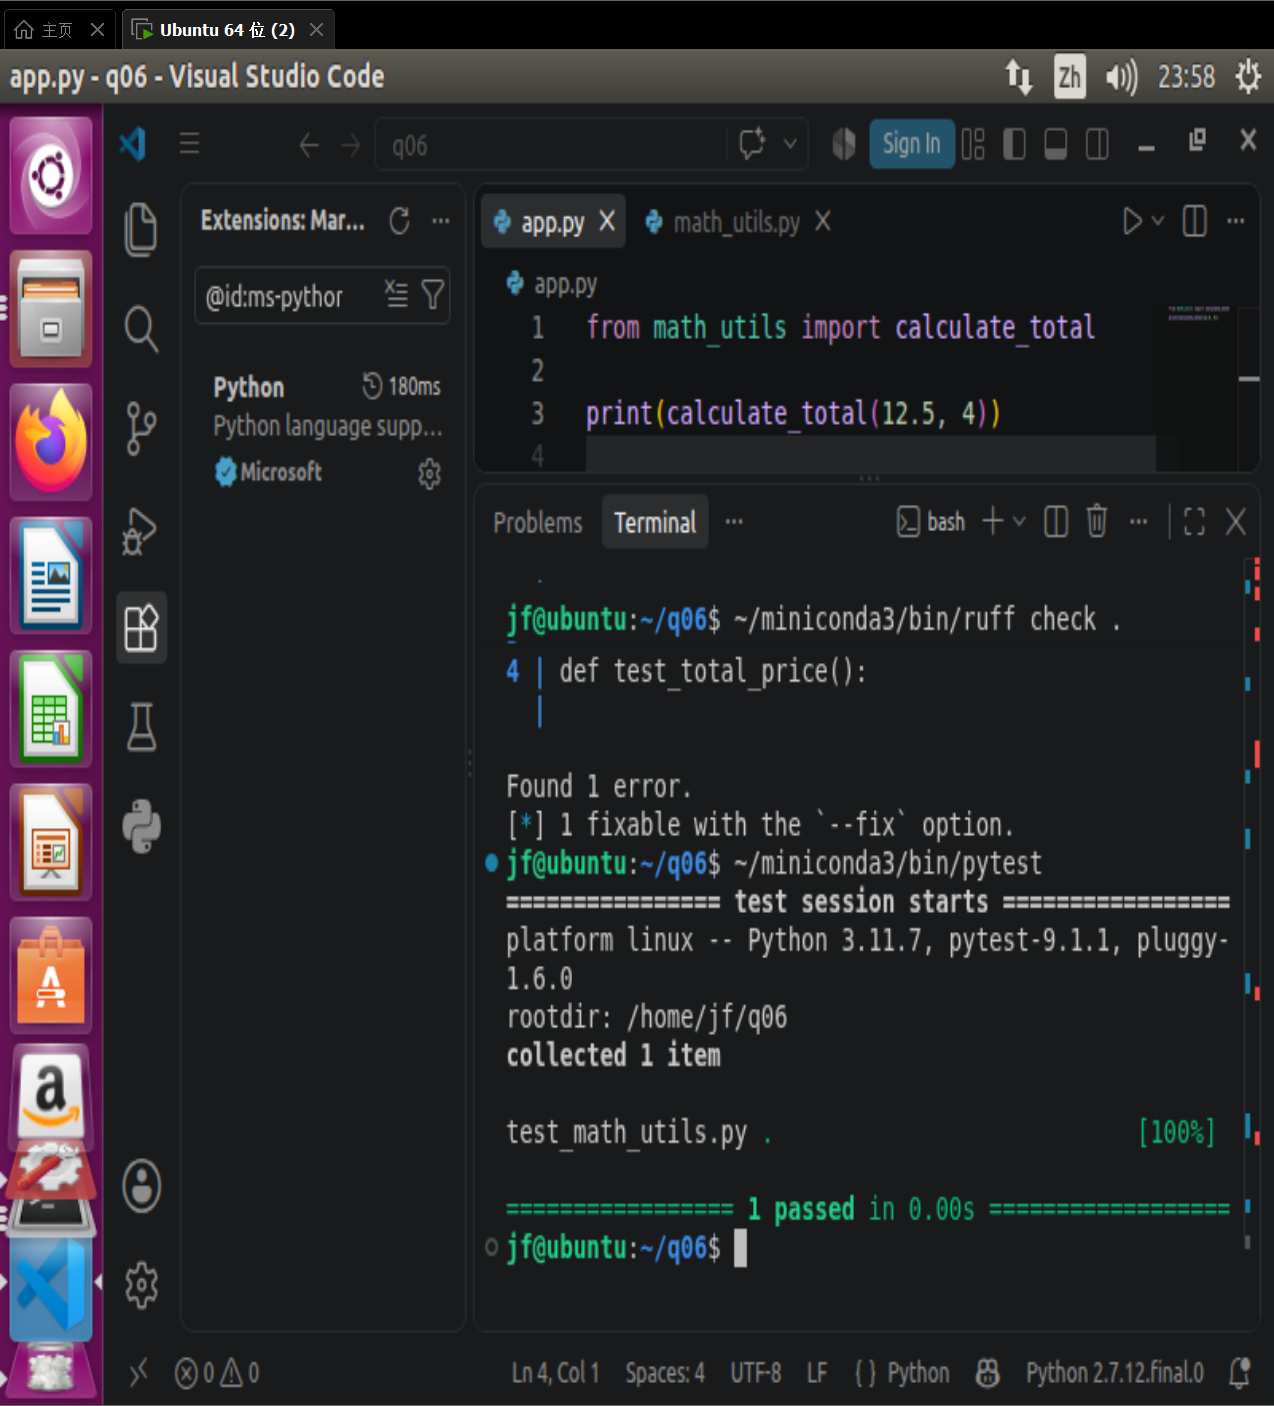
\includegraphics[width=0.9\textwidth]{q06_pytest.png}
    \caption{pytest 运行：1 passed}
    \label{fig:q06_pytest}
\end{figure}

\subsubsection*{运行结果与小结}

通过 VS Code 的 Python 语言服务器完成了语义重构：跳转到定义、查找引用、重命名符号 total\_price $\to$ calculate\_total 三处引用同步更新，验证了语言服务器"基于语义而非文本匹配"的代码感知能力。环境方面，由于系统 Python 3.5 过老且缺 ruff，安装了 Miniconda（Python 3.11.7）并安装 ruff、pytest；ruff 准确发现并（配合 --fix）删除了 app.py 中未使用的 import os，最终 ruff check 全部通过、pytest 1 个用例通过。整体体现了"编辑环境 + 静态检查 + 单元测试"的开发反馈闭环。

% ==================== 第 7 题 ====================
\subsection{第 7 题：用调试器定位归并排序缺陷}

\textbf{题目}：将给定代码保存为 q07/merge\_sort.py，运行并确认结果错误；使用 pdb 或 IDE debugger，在 merge 中设置断点，观察 $i$、$j$、left[$i$]、right[$j$] 定位缺陷；做最小修复（不得使用 sorted）；使用 pytest 增加两个测试并通过。

\begin{figure}[H]
    \centering
    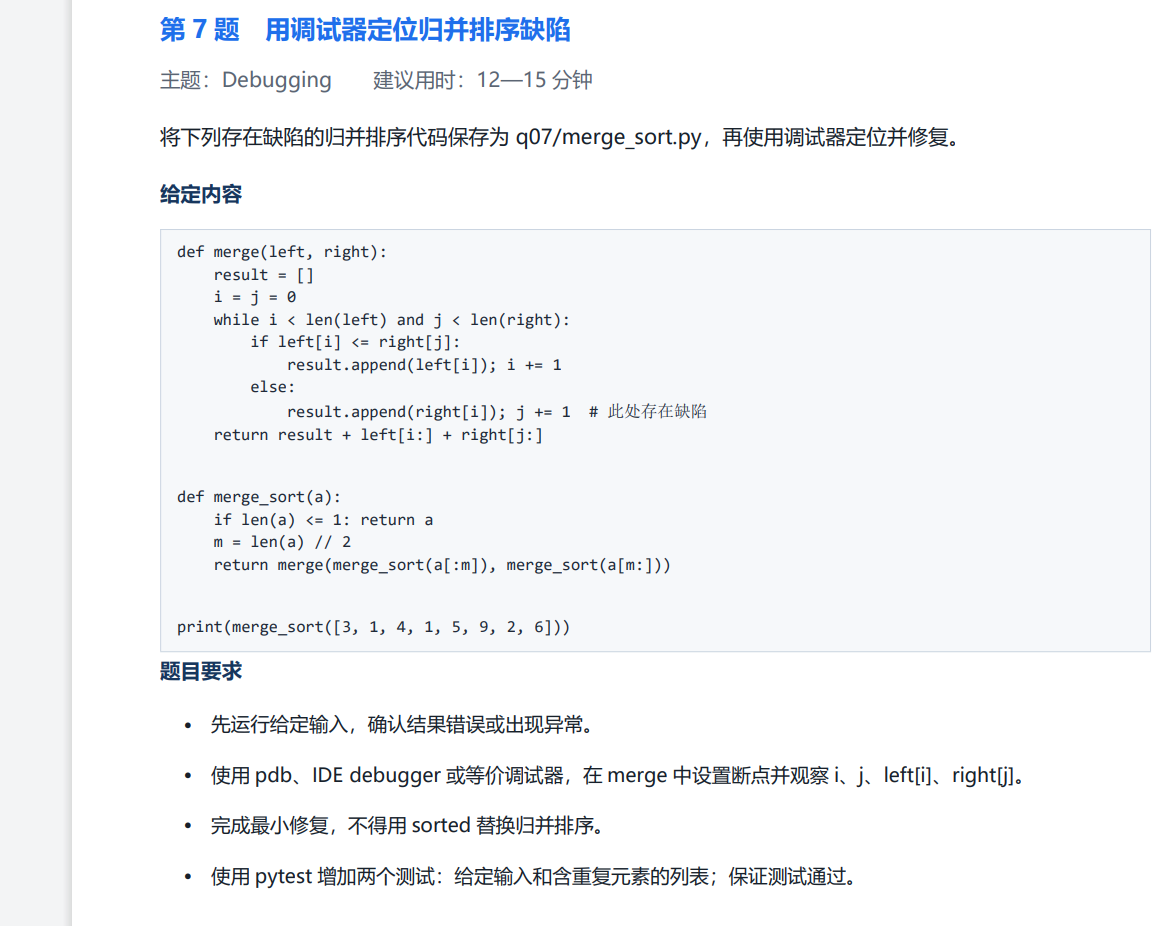
\includegraphics[width=0.9\textwidth]{q07_question.png}
    \caption{第 7 题题目要求}
    \label{fig:q07_question}
\end{figure}

\subsubsection*{作答过程与关键代码}

初始代码（含缺陷，保存为 q07/merge\_sort.py）：

\begin{lstlisting}[language=Python, caption={merge\_sort.py 初始代码（含缺陷）}]
def merge(left, right):
    result = []
    i = j = 0
    while i < len(left) and j < len(right):
        if left[i] <= right[j]:
            result.append(left[i]); i += 1
        else:
            result.append(right[i]); j += 1  # 此处存在缺陷
    return result + left[i:] + right[j:]

def merge_sort(a):
    if len(a) <= 1: return a
    m = len(a) // 2
    return merge(merge_sort(a[:m]), merge_sort(a[m:]))

print(merge_sort([3, 1, 4, 1, 5, 9, 2, 6]))
\end{lstlisting}

\begin{figure}[H]
    \centering
    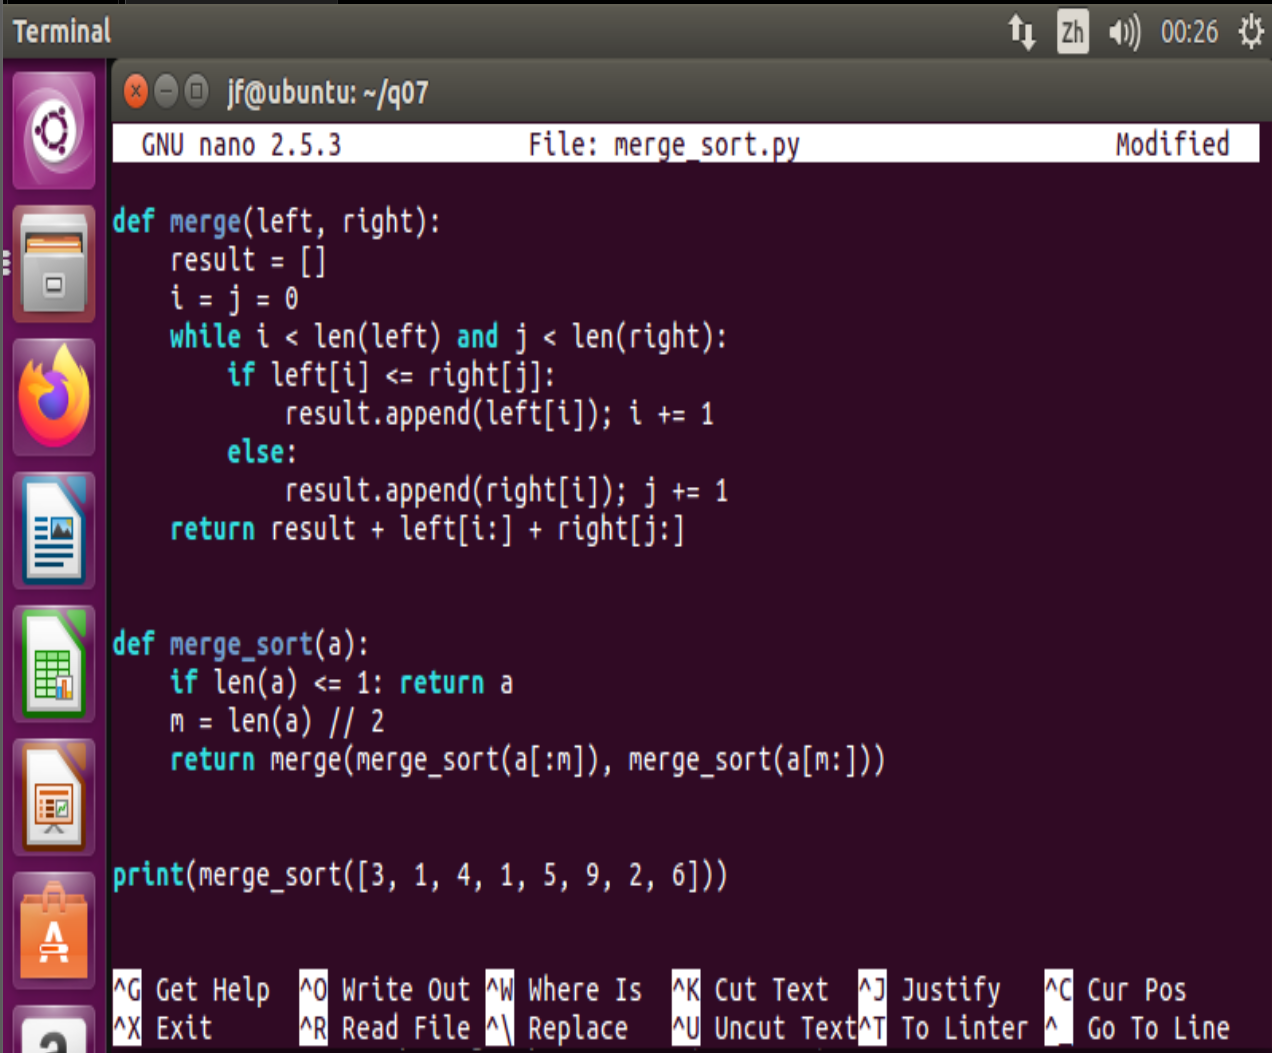
\includegraphics[width=0.9\textwidth]{q07_code_bug.png}
    \caption{nano 中编辑含缺陷的 merge\_sort.py（else 分支误用 right[i]）}
    \label{fig:q07_code_bug}
\end{figure}

首先运行初始代码确认结果错误，并启动 pdb 调试器设置断点：

\begin{lstlisting}[language=bash, caption={运行初始代码，结果错误}]
$ python3 merge_sort.py
[1, 5, 4, 3, 4, 5, 6, 9]   # 期望 [1, 1, 2, 3, 4, 5, 6, 9]，排序结果错误
\end{lstlisting}

\begin{figure}[H]
    \centering
    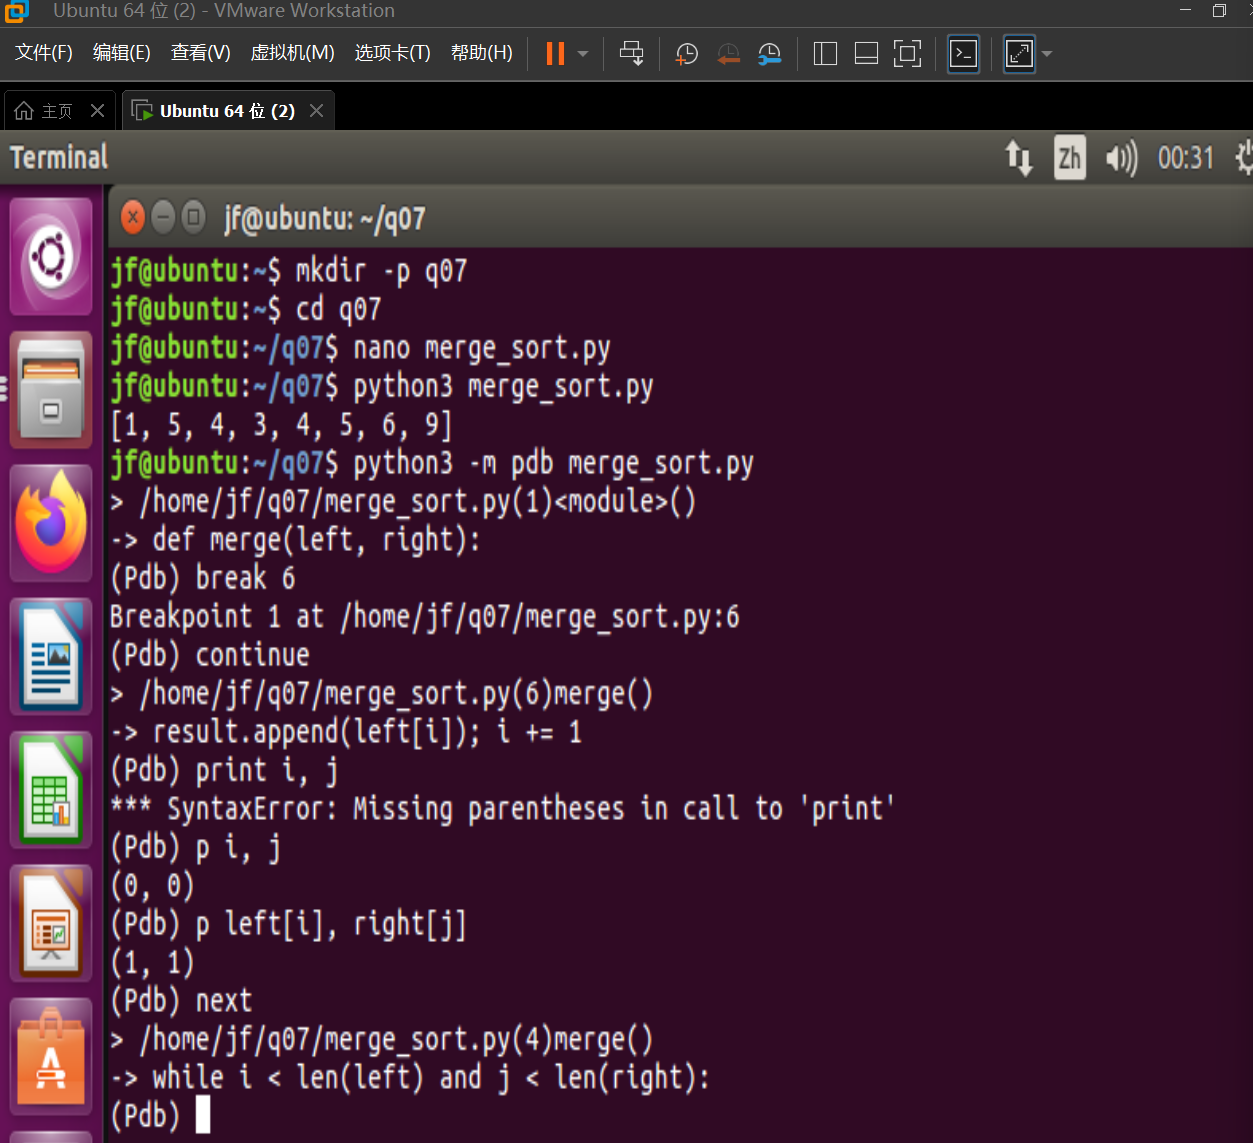
\includegraphics[width=0.9\textwidth]{q07_pdb_start.png}
    \caption{运行确认错误结果，进入 pdb 并在 merge 中设置断点}
    \label{fig:q07_pdb_start}
\end{figure}

在 merge 的循环中单步执行，观察索引 $i$、$j$ 与待比较元素 left[$i$]、right[$j$] 的变化。当程序停在缺陷行（result.append(right[$i$])）时，关键的取证结果如下：

\begin{lstlisting}[language=bash, caption={pdb 中断点取证}]
(Pdb) p i, j
(1, 0)
(Pdb) p right
[1, 4]
(Pdb) p right[i], right[j]     # 关键：两者不同！
(4, 1)
\end{lstlisting}

\begin{figure}[H]
    \centering
    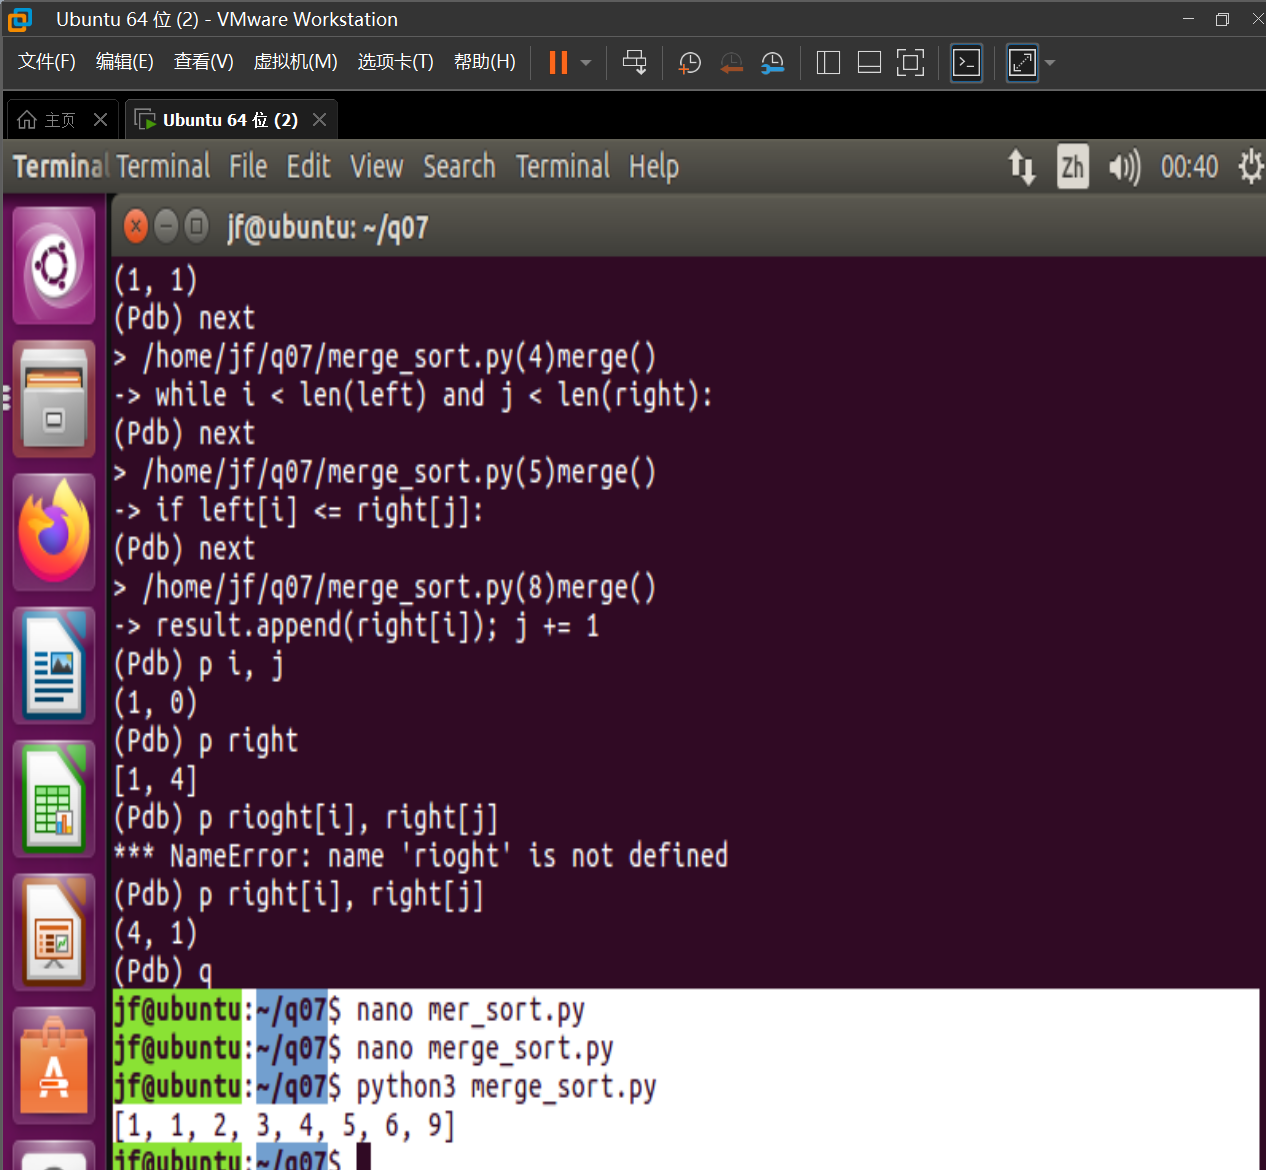
\includegraphics[width=0.9\textwidth]{q07_pdb_evidence.png}
    \caption{pdb 取证：i=1、j=0 时 right[i]=4 而 right[j]=1（右上为修复后正确输出）}
    \label{fig:q07_pdb_evidence}
\end{figure}

\textbf{缺陷定位}：当 $i=1,\ j=0$ 时，本应将 right 中最小的元素 right[$j$]=right[0]=1 追加到结果，但代码写成了 right[$i$]=right[1]=4，取错了元素。原因是 merge 的 else 分支把 left 的索引 $i$ 误用于 right，属于复制粘贴错误。修复方法：把 right[$i$] 改为 right[$j$]（最小修改，仅改一个字符）。

\begin{lstlisting}[language=Python, caption={最小修复：right[i] 改为 right[j]}]
        else:
            result.append(right[j]); j += 1   # 修复后
\end{lstlisting}

\begin{figure}[H]
    \centering
    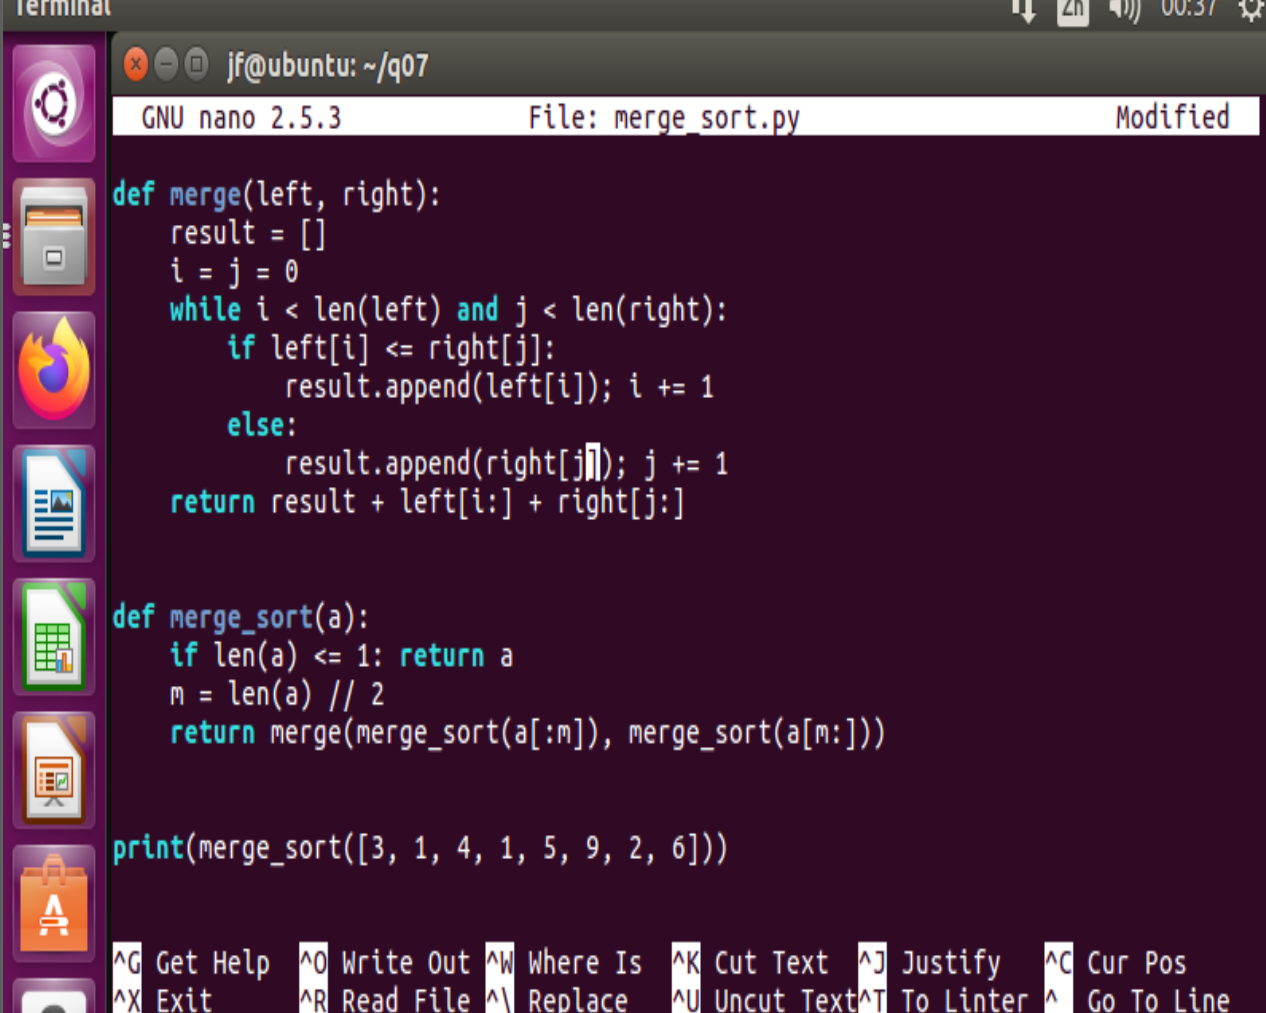
\includegraphics[width=0.9\textwidth]{q07_code_fixed.png}
    \caption{nano 中已改为 right[j]（最小修复）}
    \label{fig:q07_code_fixed}
\end{figure}

修复后重新运行，结果正确，并编写 pytest 测试文件：

\begin{lstlisting}[language=Python, caption={pytest 测试用例}]
from merge_sort import merge_sort

def test_given_input():
    assert merge_sort([3, 1, 4, 1, 5, 9, 2, 6]) == [1, 1, 2, 3, 4, 5, 6, 9]

def test_duplicate_elements():
    assert merge_sort([2, 2, 1, 3, 1, 2, 1]) == [1, 1, 1, 2, 2, 2, 3]
\end{lstlisting}

\begin{figure}[H]
    \centering
    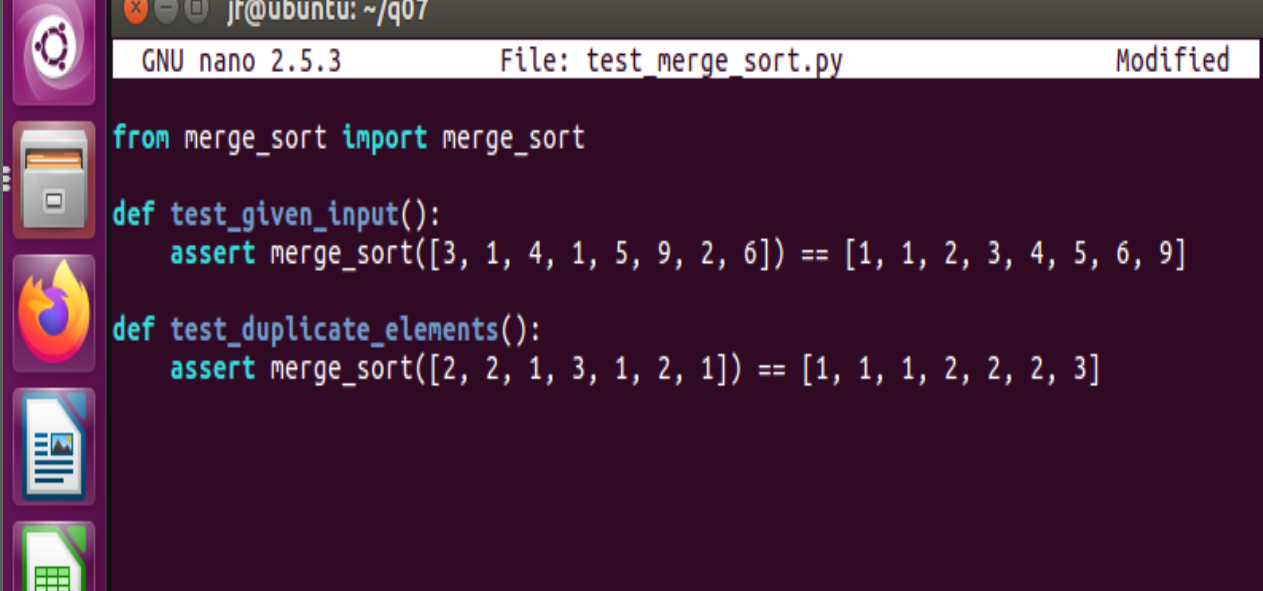
\includegraphics[width=0.9\textwidth]{q07_test_file.png}
    \caption{nano 中编写 test\_merge\_sort.py（两个测试用例）}
    \label{fig:q07_test_file}
\end{figure}

\begin{figure}[H]
    \centering
    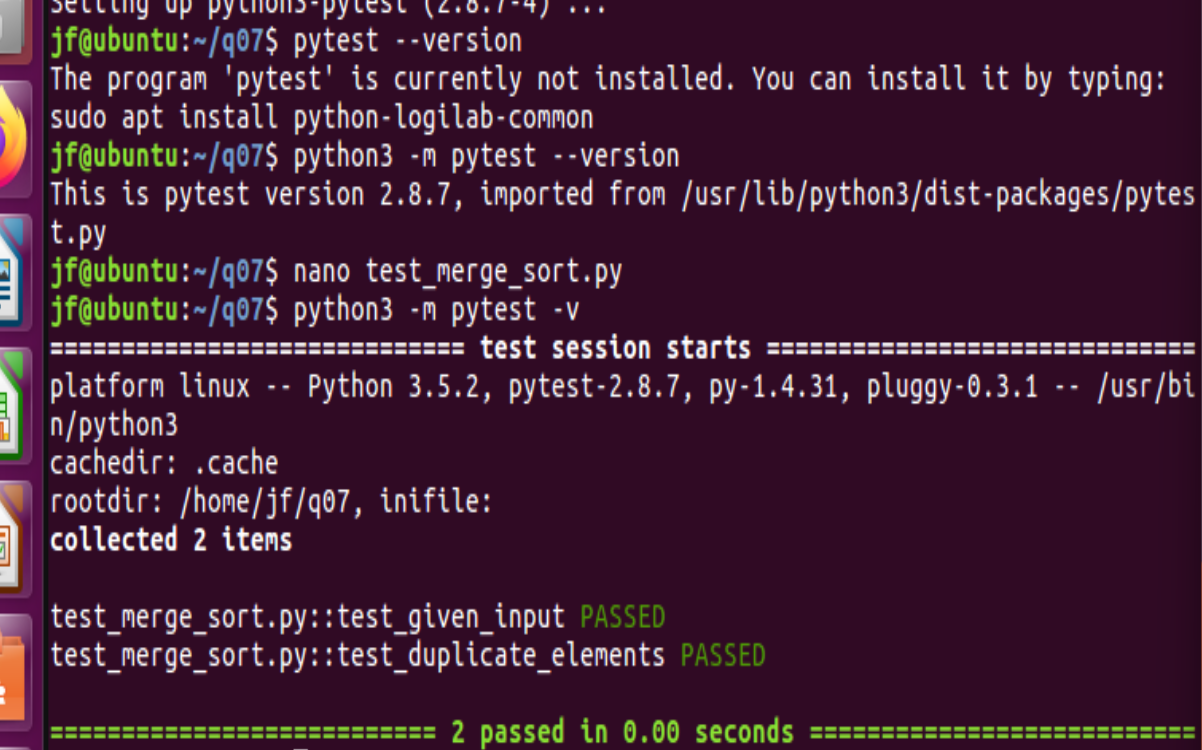
\includegraphics[width=0.9\textwidth]{q07_pytest.png}
    \caption{pytest 运行，2 个用例全部通过}
    \label{fig:q07_pytest}
\end{figure}

\subsubsection*{运行结果与小结}

通过 pdb 观察 left[$i$]、right[$j$] 与实际取用的 right[$i$]，确认了缺陷来源：else 分支误用左半边的索引 $i$ 访问 right 列表。修复为 right[$j$] 后排序正确，pytest 的两个用例（给定输入、含重复元素）均通过，说明修复没有破坏边界情况。

% ==================== 第 8 题 ====================
\subsection{第 8 题：先测量，再优化慢速词频程序}

\textbf{题目}：在 q08 中完成：(1) 用 generate\_words.py 生成含 30000 个随机词（取自 1000 个词汇）的 words.txt；(2) 运行低效的 wordfreq.py，用 time 命令记录两次耗时；(3) 用 cProfile 定位主要耗时位置；(4) 优化程序（不得改变最终 count，不得写死 1000）；(5) 相同输入再运行两次，计算优化前后中位数与加速比。

\begin{figure}[H]
    \centering
    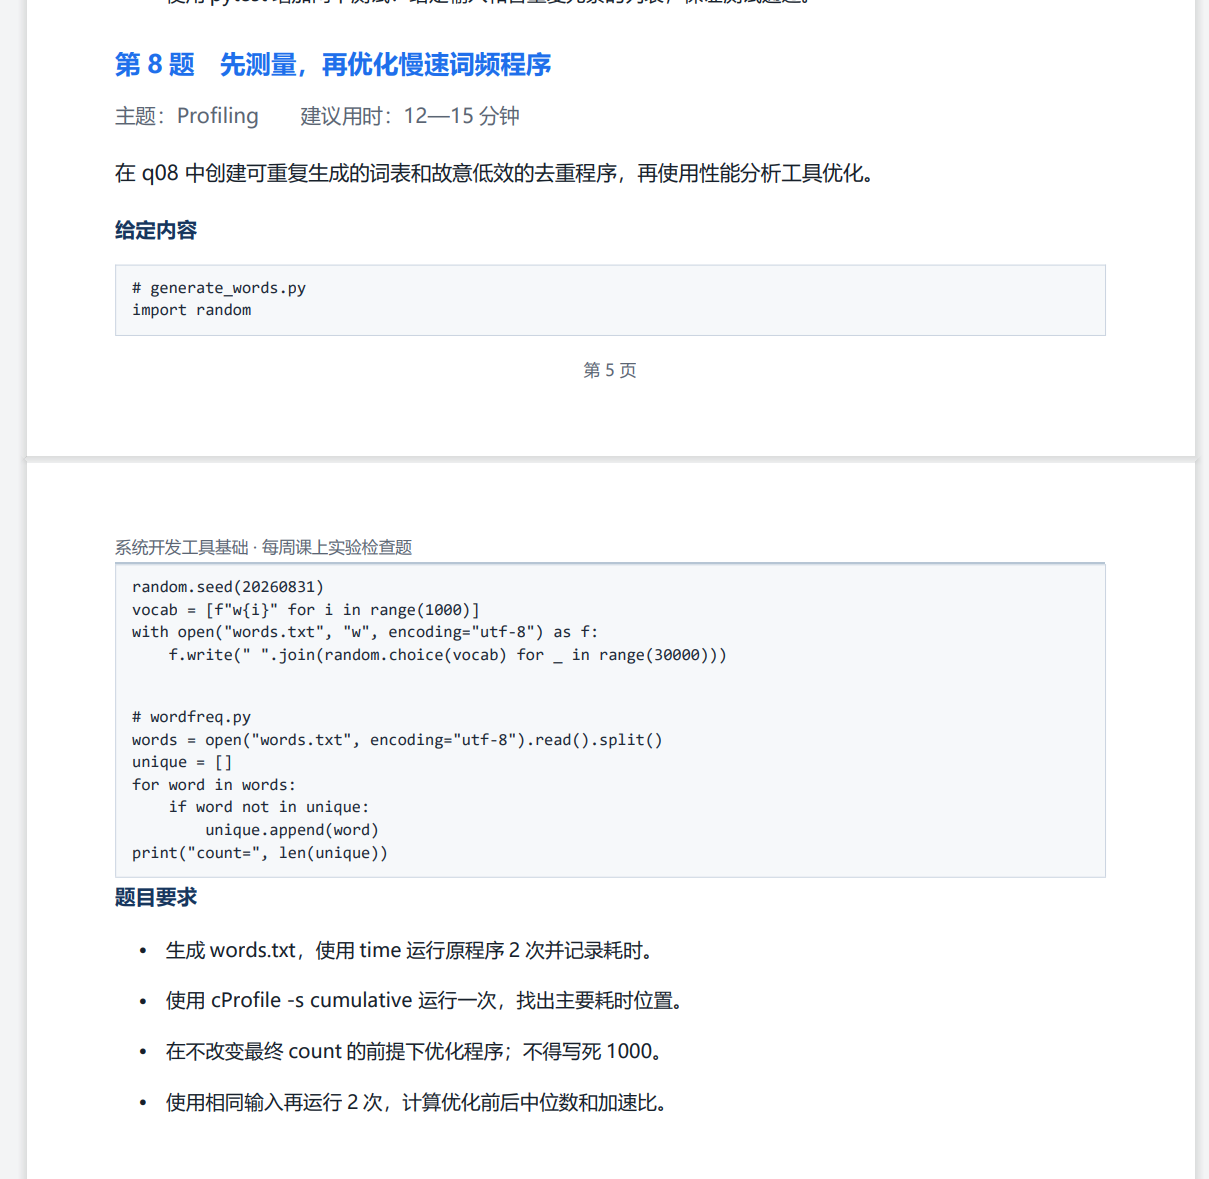
\includegraphics[width=0.9\textwidth]{q08_question.png}
    \caption{第 8 题题目要求}
    \label{fig:q08_question}
\end{figure}

\subsubsection*{作答过程与关键代码}

生成随机词数据。本机 Python 为 3.5，不支持 f-string，改为 .format 写法：

\begin{lstlisting}[language=Python, caption={generate\_words.py（生成 30000 个随机词）}]
import random
random.seed(20260831)
vocab = ["w{}".format(i) for i in range(1000)]
with open("words.txt", "w", encoding="utf-8") as f:
    f.write(" ".join(random.choice(vocab) for _ in range(30000)))
\end{lstlisting}

\begin{figure}[H]
    \centering
    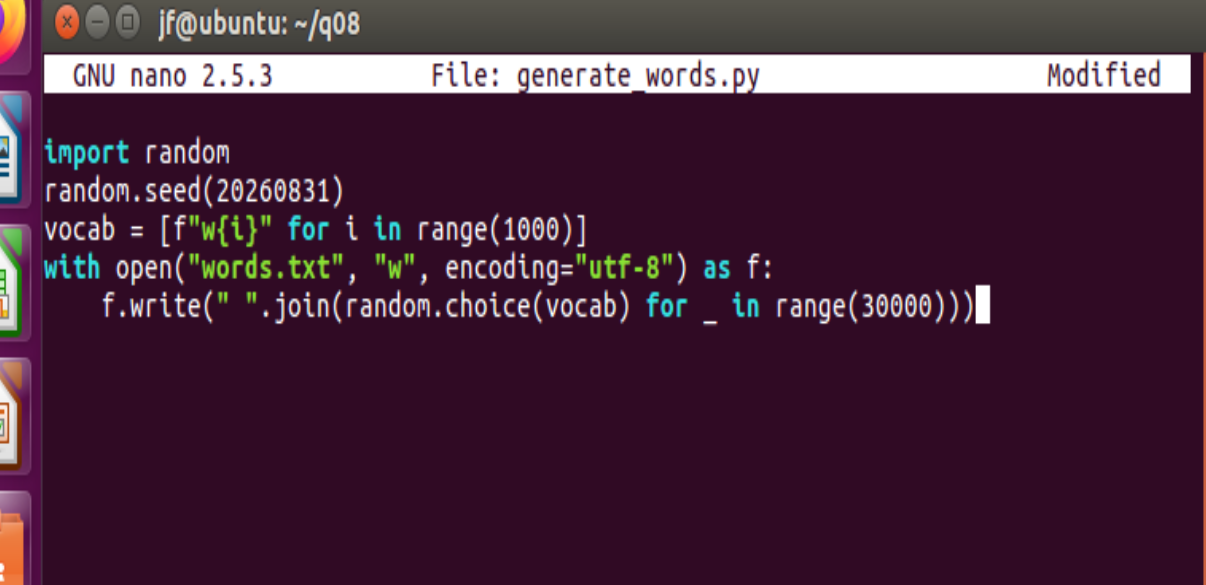
\includegraphics[width=0.9\textwidth]{q08_gen_words.png}
    \caption{nano 中编辑 generate\_words.py}
    \label{fig:q08_gen_words}
\end{figure}

运行 generate\_words.py 生成 words.txt。低效版 wordfreq.py 用 list 去重，查找为线性 $O(n)$，总体 $O(n^2)$：

\begin{lstlisting}[language=Python, caption={wordfreq.py 低效版}]
words = open("words.txt", encoding="utf-8").read().split()
unique = []
for word in words:
    if word not in unique:      # list 线性查找，低效
        unique.append(word)
print("count=", len(unique))
\end{lstlisting}

\begin{figure}[H]
    \centering
    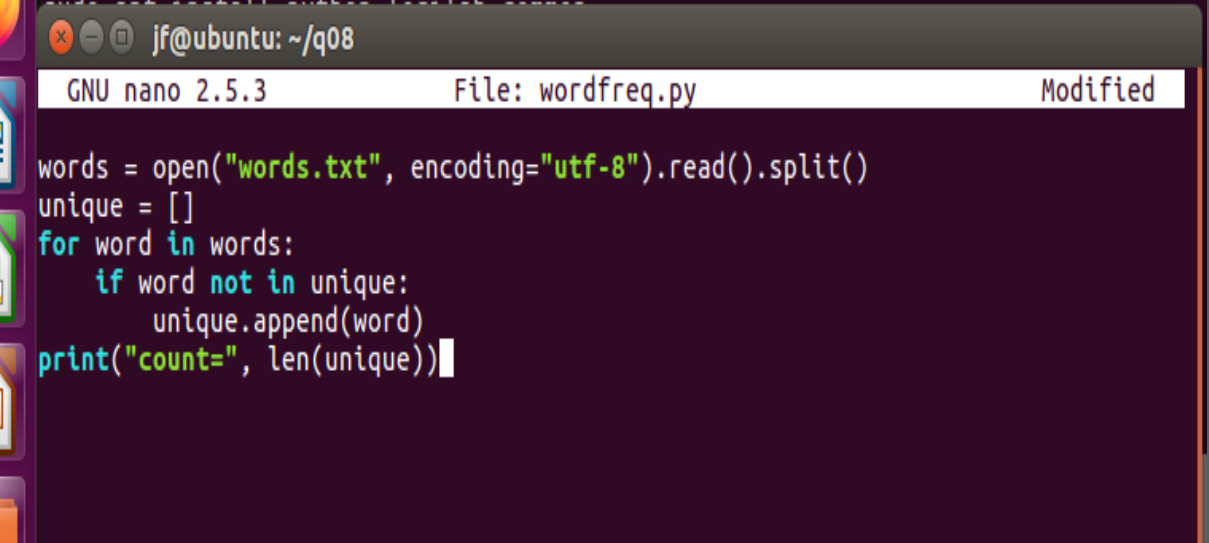
\includegraphics[width=0.9\textwidth]{q08_code_low.png}
    \caption{nano 中编辑 wordfreq.py 低效版}
    \label{fig:q08_code_low}
\end{figure}

优化前使用 time 命令测量两次：

\begin{lstlisting}[language=bash, caption={优化前两次计时}]
$ time python3 wordfreq.py
count= 1000
real    0m0.121s
$ time python3 wordfreq.py
count= 1000
real    0m0.116s
\end{lstlisting}

\begin{figure}[H]
    \centering
    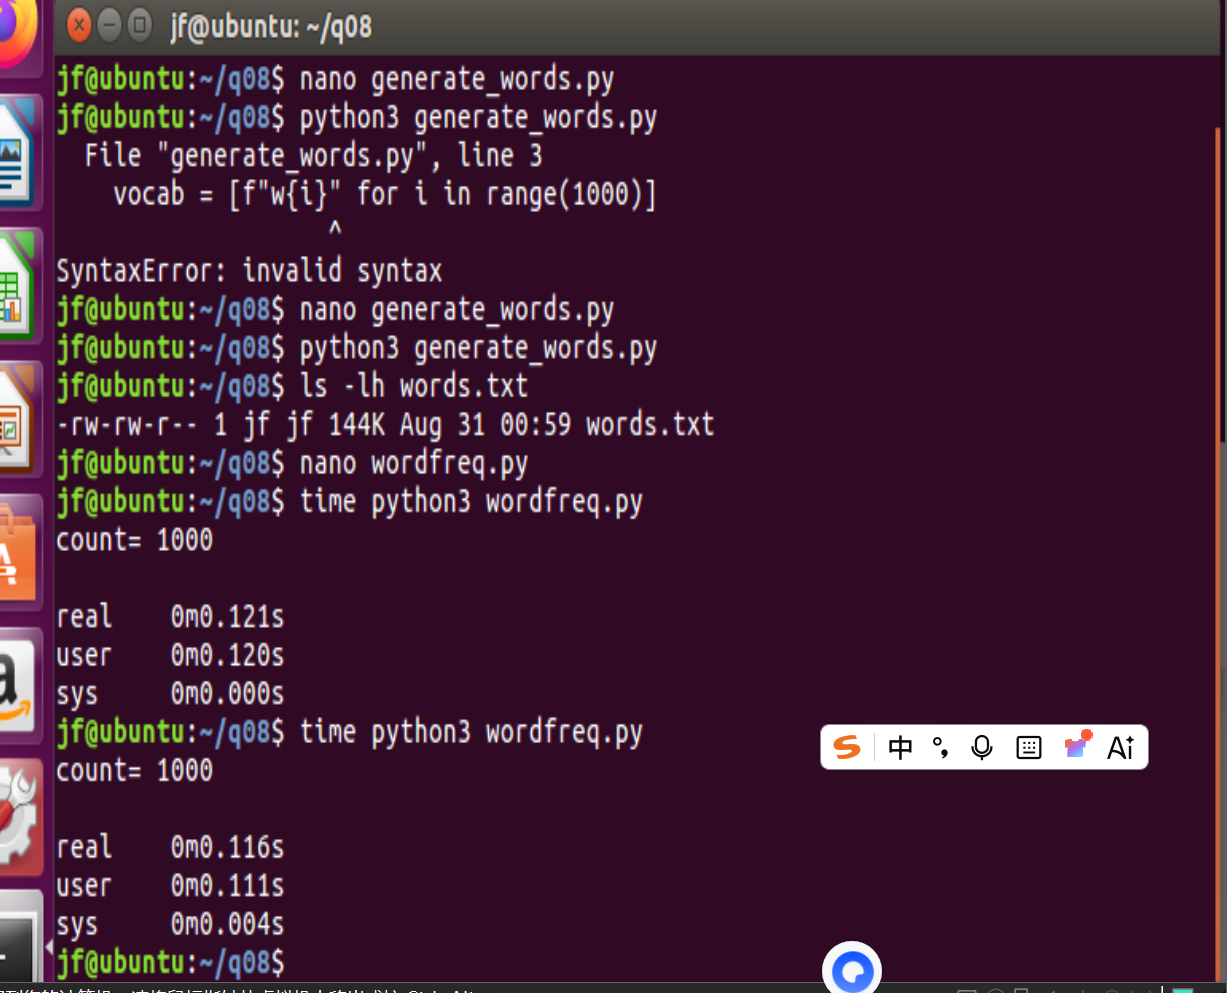
\includegraphics[width=0.9\textwidth]{q08_run_before.png}
    \caption{生成 words.txt，并记录优化前两次 time 耗时}
    \label{fig:q08_run_before}
\end{figure}

使用 cProfile 定位耗时：

\begin{lstlisting}[language=bash, caption={cProfile 性能分析}]
$ python3 -m cProfile -s cumulative wordfreq.py
1012 function calls in 0.108 seconds
ncalls   tottime  percall  cumtime  percall  filename:lineno(function)
1        0.000    0.000    0.108    0.108    {built-in method builtins.exec}
1        0.106    0.106    0.108    0.108    wordfreq.py:1(<module>)   # 瓶颈所在
1000     0.000    0.000    0.000    0.000    {method 'append' of 'list' objects}
\end{lstlisting}

\begin{figure}[H]
    \centering
    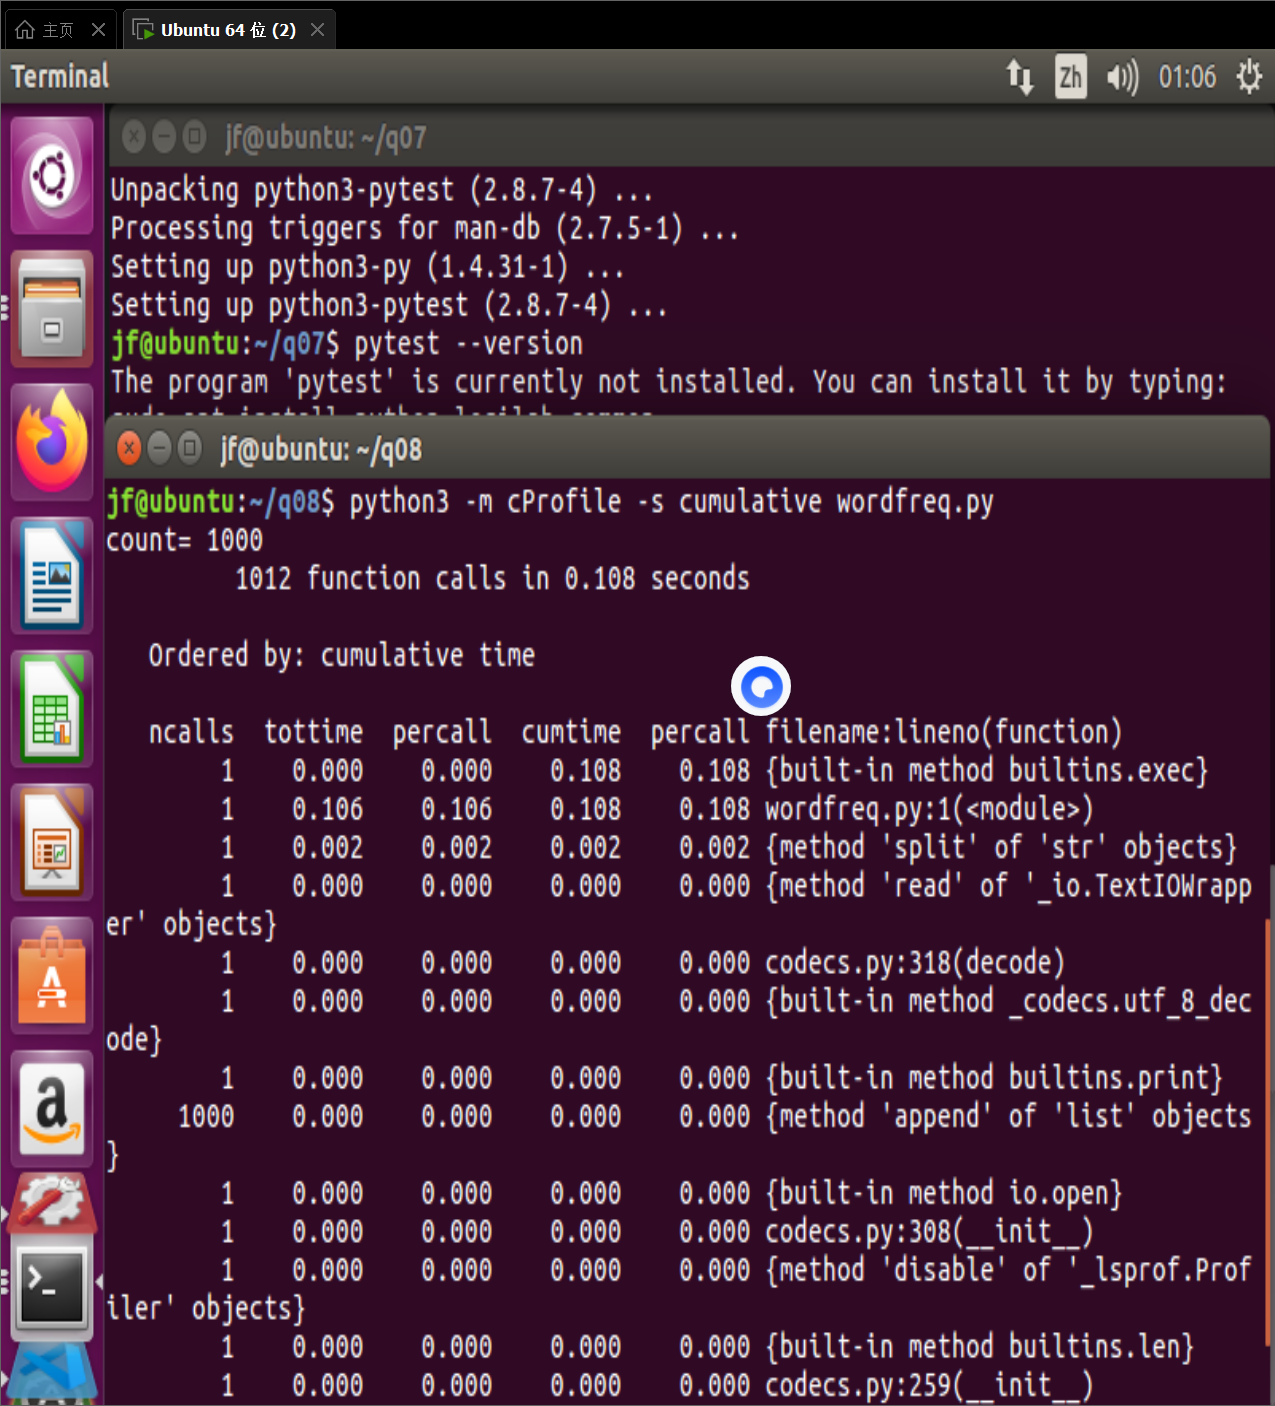
\includegraphics[width=0.9\textwidth]{q08_cprofile.png}
    \caption{cProfile 定位：wordfreq.py 顶层循环占 98\% 耗时}
    \label{fig:q08_cprofile}
\end{figure}

\textbf{定位结论}：总耗时 0.108s，其中 wordfreq.py 顶层循环自身耗时 0.106s、占比约 98\%，说明慢的是主循环中 \texttt{word not in unique} 对 list 的线性查找。优化方案：将去重容器由 list 改为 set（哈希表，查找 $O(1)$），程序整体由 $O(n^2)$ 降为 $O(n)$。

\begin{lstlisting}[language=Python, caption={wordfreq.py 优化版（set 去重）}]
words = open("words.txt", encoding="utf-8").read().split()
unique = set(words)             # set 哈希查找 O(1)
print("count=", len(unique))
\end{lstlisting}

\begin{figure}[H]
    \centering
    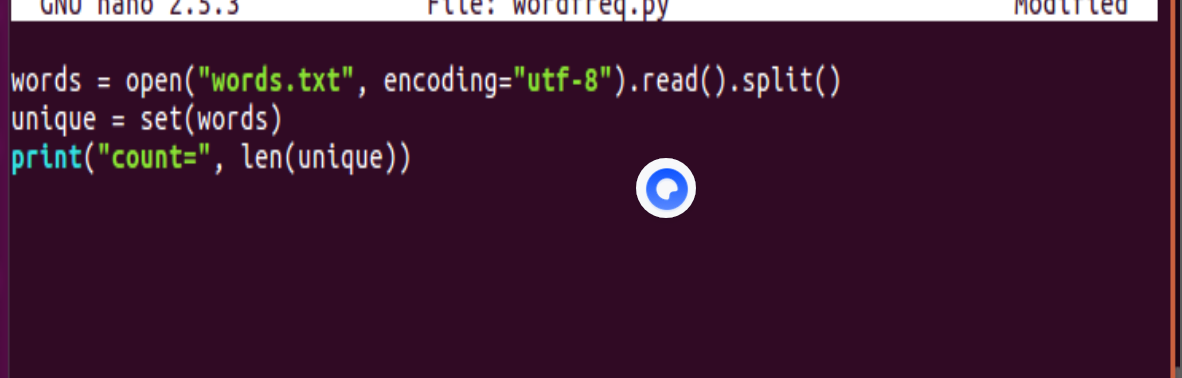
\includegraphics[width=0.9\textwidth]{q08_code_opt.png}
    \caption{nano 中编辑 wordfreq.py 优化版（set 去重）}
    \label{fig:q08_code_opt}
\end{figure}

优化后 count 保持不变（仍为 1000），并再次计时两次：

\begin{lstlisting}[language=bash, caption={优化后两次计时}]
$ python3 wordfreq.py
count= 1000
$ time python3 wordfreq.py
count= 1000
real    0m0.011s
$ time python3 wordfreq.py
count= 1000
real    0m0.012s
\end{lstlisting}

\begin{figure}[H]
    \centering
    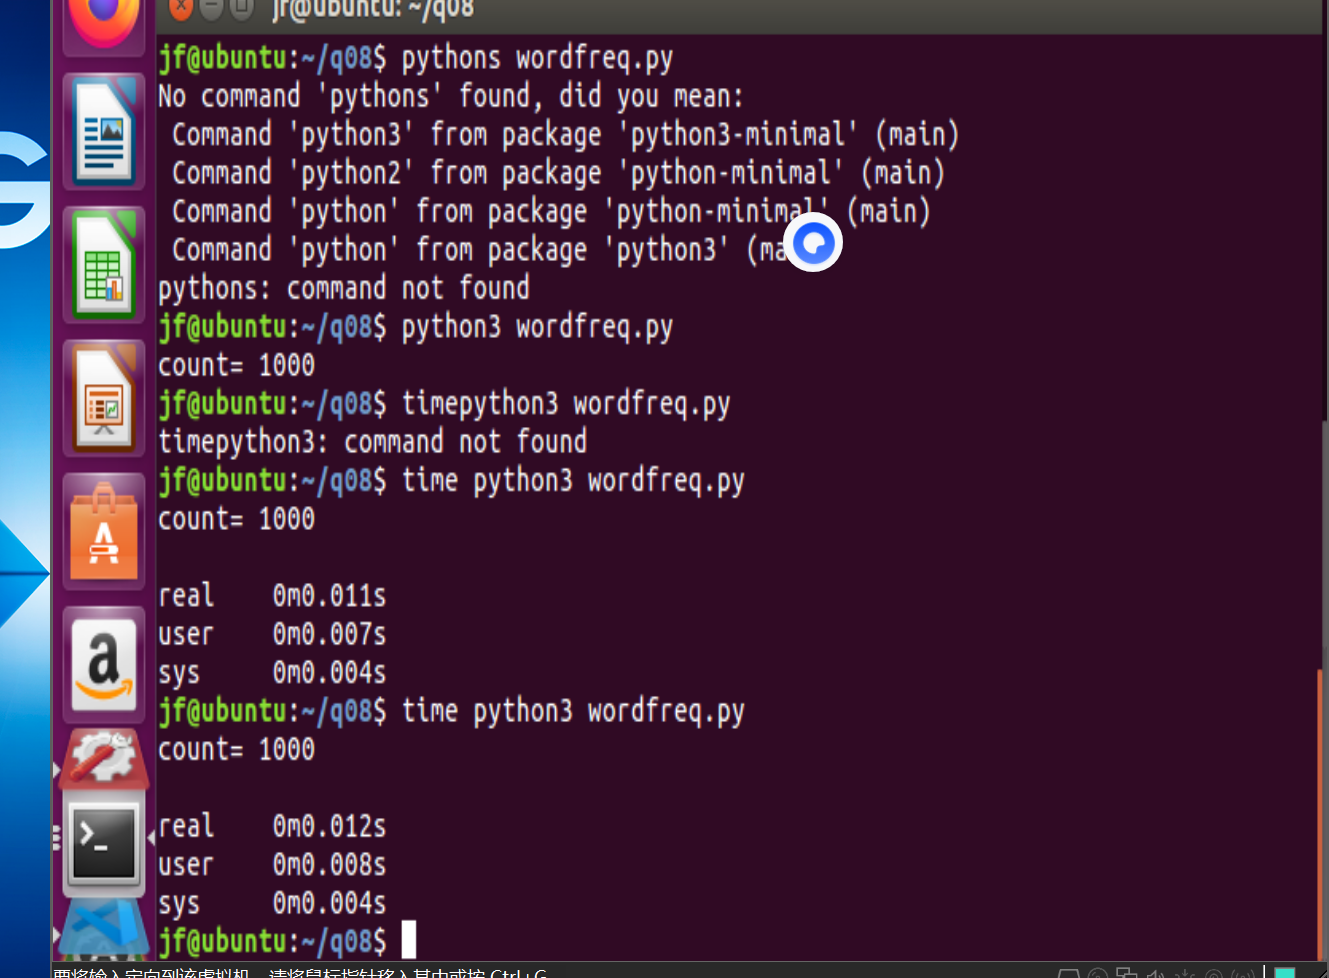
\includegraphics[width=0.9\textwidth]{q08_run_after.png}
    \caption{优化后两次 time 计时（0.011s、0.012s）}
    \label{fig:q08_run_after}
\end{figure}

\subsubsection*{运行结果与性能对比}

优化前后各运行两次的 real 时间及中位数如下：

\begin{table}[H]
    \centering
    \begin{tabular}{ccc}
        \toprule
        阶段 & real 时间（两次） & 中位数 \\
        \midrule
        优化前（list 查找） & 0.121s、0.116s & 0.1185s \\
        优化后（set 查找）  & 0.011s、0.012s  & 0.0115s \\
        \bottomrule
    \end{tabular}
    \caption{优化前后耗时对比}
    \label{tab:q08_compare}
\end{table}

加速比计算：$0.1185 \div 0.0115 \approx 10.3$，优化后程序提速约 \textbf{10.3 倍}。整个过程中最终 count 始终为 1000，符合题目"不得改变 count、不得写死 1000"的要求。

% ----------------------------------------------------------------------------
% 2. 课后练习内容和结果
% ----------------------------------------------------------------------------
\section{课后练习内容和结果}

% ==================== 练习 1：信号与任务控制 ====================
\subsection{信号与任务控制}

\textbf{题目}：在终端里启动一个 sleep 10000 任务，用 Ctrl-Z 把它挂起，再用 bg 让它继续在后台运行。然后使用 pgrep 找到它的 pid，再用 pkill 把它杀掉，整个过程都不要手动输入这个 pid。（提示：试试 -af 参数）

\begin{figure}[H]
    \centering
    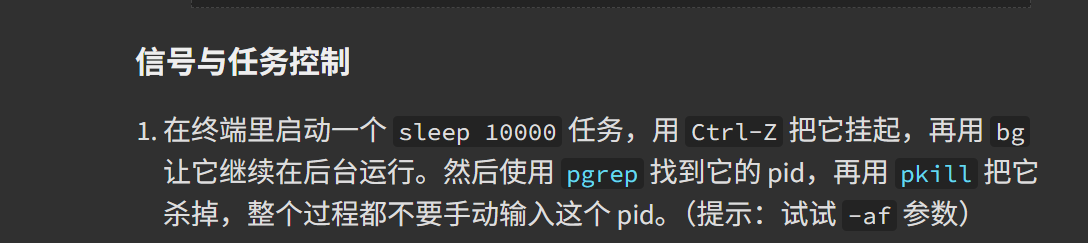
\includegraphics[width=0.9\textwidth]{sig_question.png}
    \caption{练习题目要求}
    \label{fig:sig_question}
\end{figure}

\subsubsection*{作答过程与运行结果}

先启动 sleep 10000 任务，用 Ctrl-Z 挂起，bg 转后台，再用 pgrep -af 查找进程、pkill -f 按命令行匹配终止：

\begin{lstlisting}[language=bash, caption={任务控制全过程}]
$ sleep 10000
^Z
[1]+  Stopped                 sleep 10000
$ bg
[1]+ sleep 10000 &
$ pgrep -af sleep
4709 sleep 10000
$ pkill -f "sleep 10000"
[1]+  Terminated              sleep 10000
$ pgrep -af sleep
$
\end{lstlisting}

\begin{figure}[H]
    \centering
    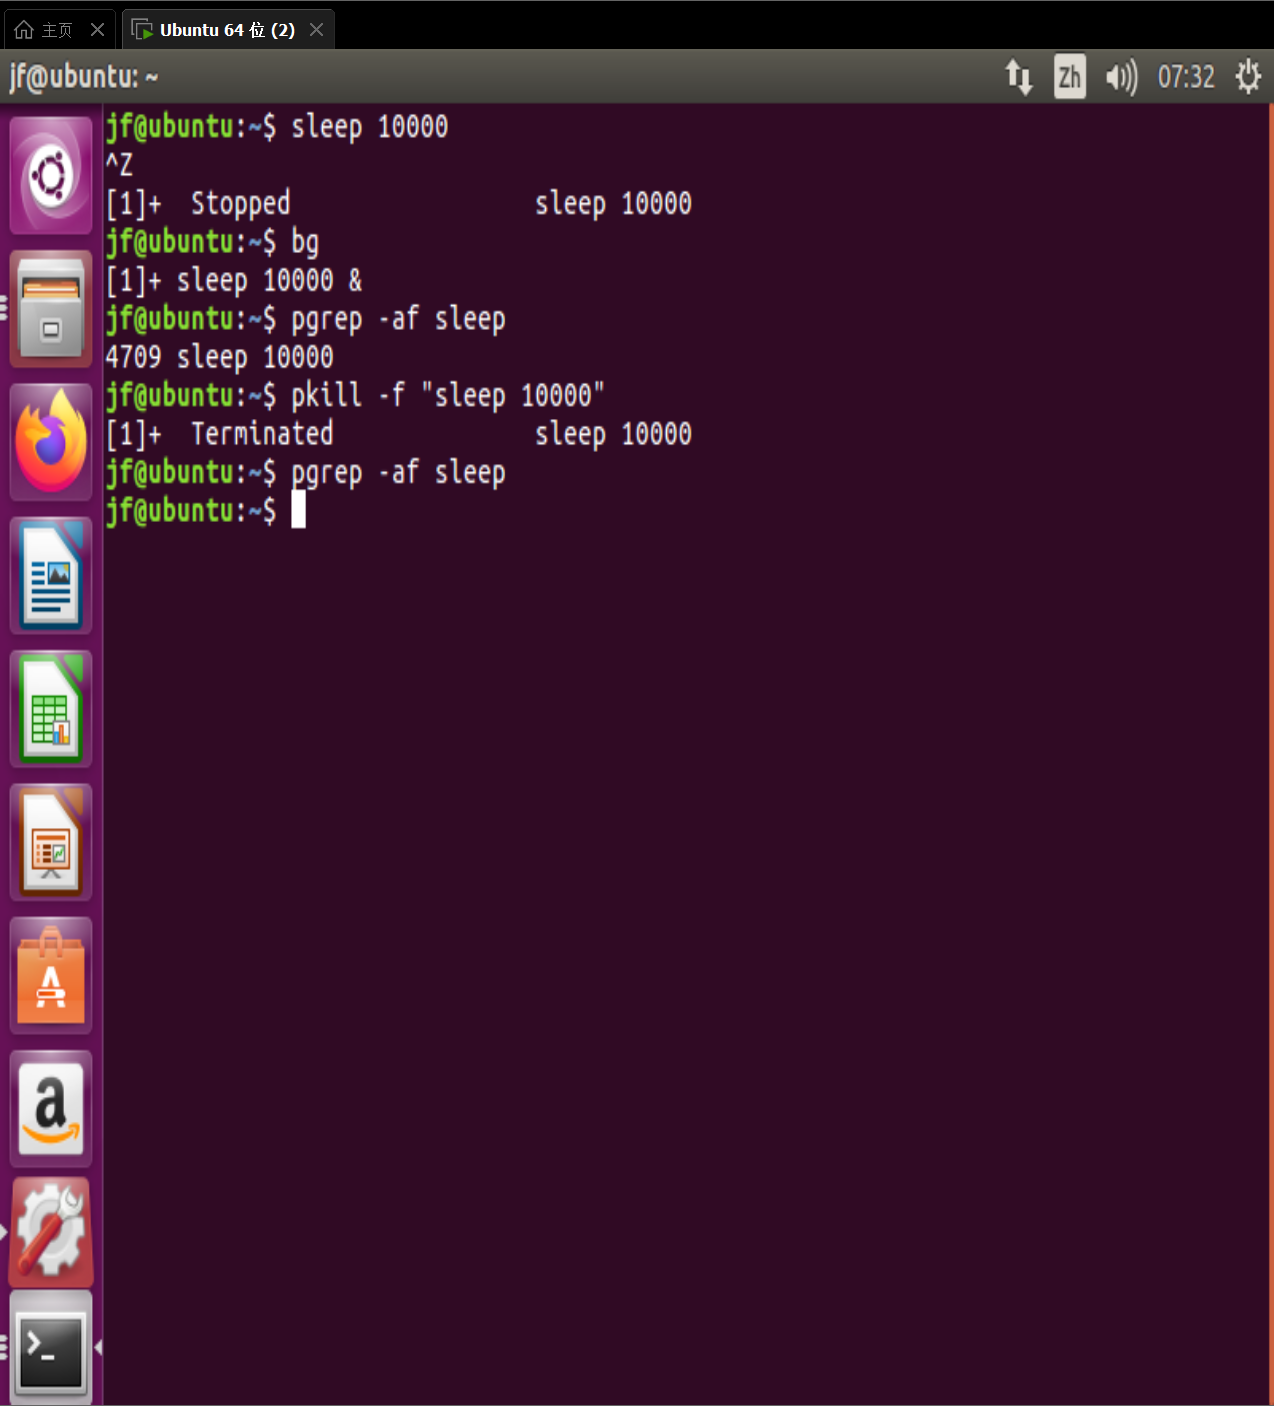
\includegraphics[width=0.9\textwidth]{sig_run.png}
    \caption{任务控制执行过程（挂起、后台、pgrep 查找、pkill 终止）}
    \label{fig:sig_run}
\end{figure}

\subsubsection*{小结}
整个过程没有手动输入 PID：pgrep -af 按命令行内容查找并显示 pid，pkill -f 用同样的命令行模式匹配后终止，最后再次 pgrep 无结果，说明任务已被成功终止。

% ==================== 练习 2：marco 与 polo ====================
\subsection{环境变量：bash 函数 marco 与 polo}

\textbf{题目}：写两个 bash 函数 marco 和 polo，行为如下：每次执行 marco 时，都要以某种方式保存当前工作目录；之后无论你切到哪个目录，只要执行 polo，它都应该把你 cd 回执行 marco 时所在的目录。可以把代码写进 marco.sh，然后通过执行 source marco.sh 把这些定义重新加载到当前 shell。

\begin{figure}[H]
    \centering
    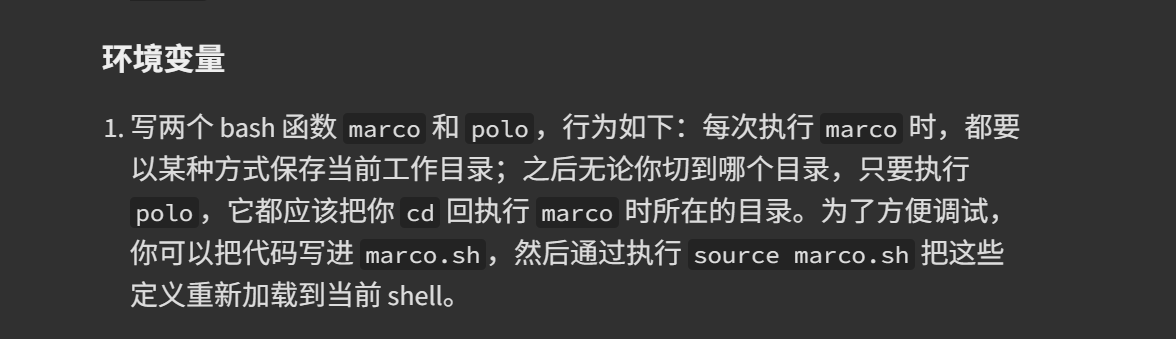
\includegraphics[width=0.9\textwidth]{marco_question.png}
    \caption{练习题目要求}
    \label{fig:marco_question}
\end{figure}

\subsubsection*{作答过程与运行结果}

\begin{lstlisting}[language=bash, caption={marco.sh：marco 保存目录，polo 返回目录}]
#!/usr/bin/env bash
marco(){
    MARCO_DIR="$PWD"
    echo "save contents: $MARCO_DIR"
}
polo(){
    if [[ -z "$MARCO_DIR" ]]; then
        echo "error, please save marco contents"
        return 1
    fi
    cd "$MARCO_DIR" && echo "return: $MARCO_DIR"
}
\end{lstlisting}

\begin{figure}[H]
    \centering
    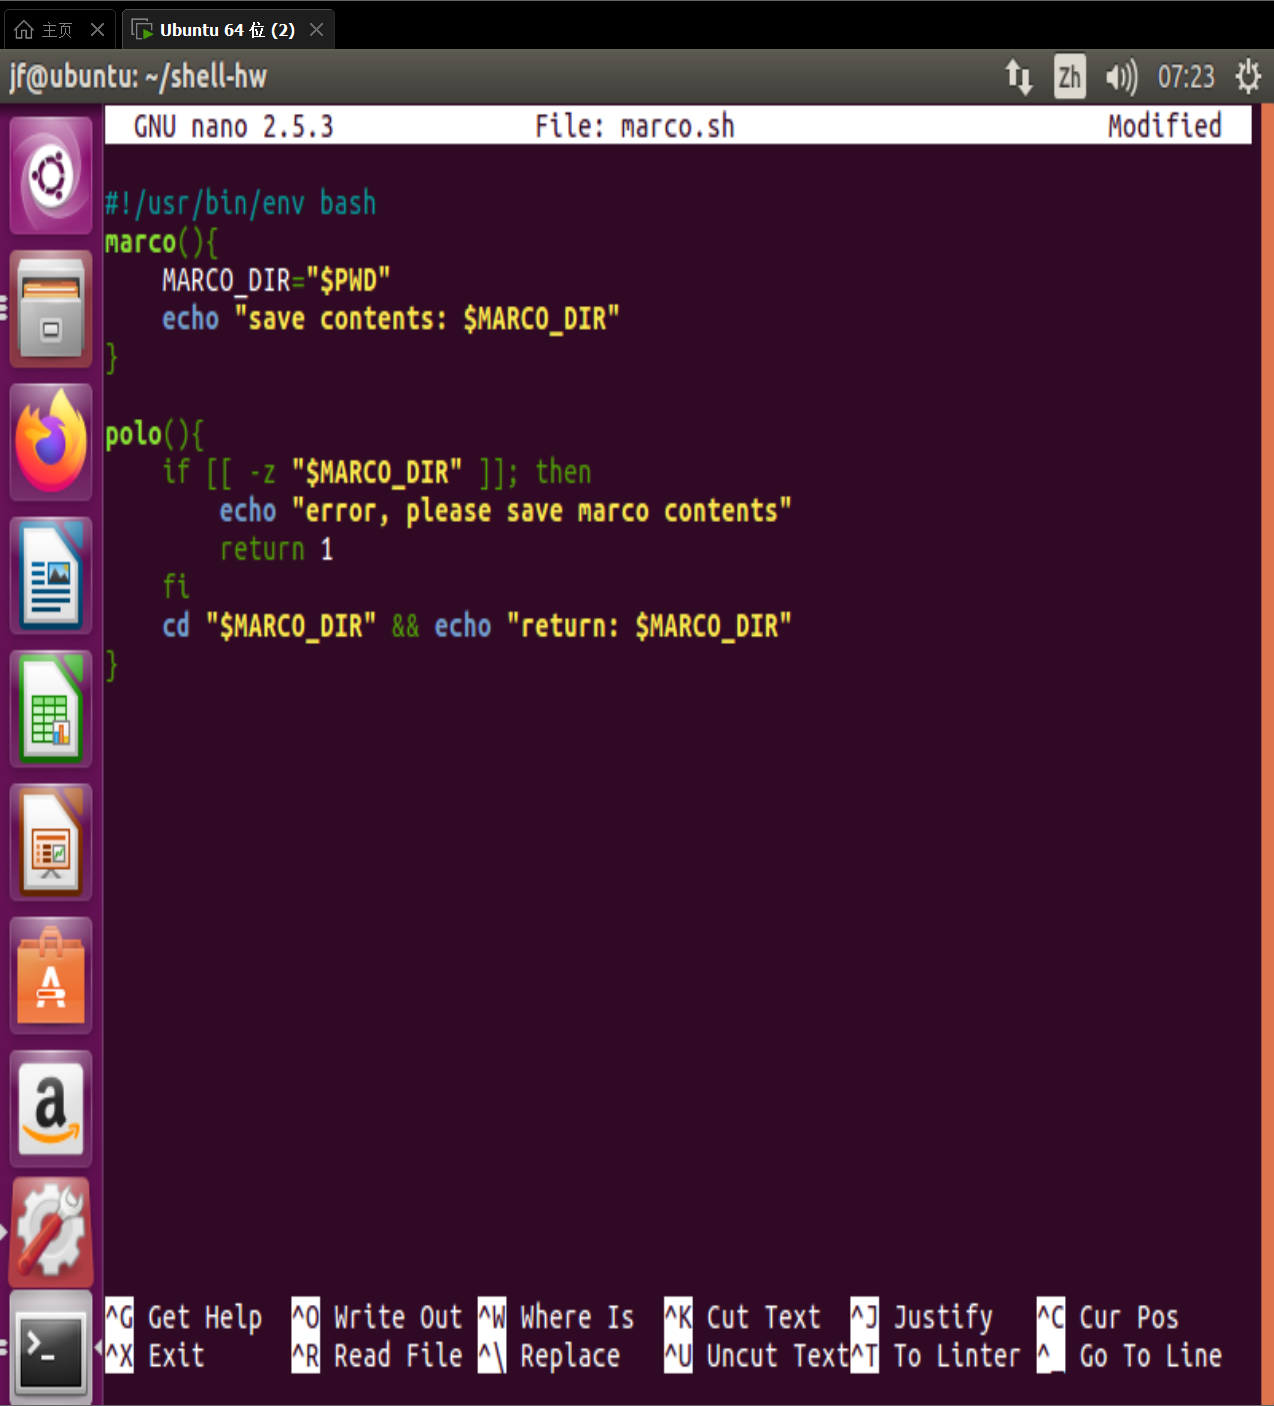
\includegraphics[width=0.9\textwidth]{marco_code.png}
    \caption{nano 中编辑 marco.sh（marco/polo 两个函数）}
    \label{fig:marco_code}
\end{figure}

\begin{lstlisting}[language=bash, caption={加载并验证 marco/polo}]
$ source marco.sh
$ cd /tmp
$ marco
save contents: /tmp
$ cd /var/log
$ polo
return: /tmp
$ pwd
/tmp
\end{lstlisting}

\begin{figure}[H]
    \centering
    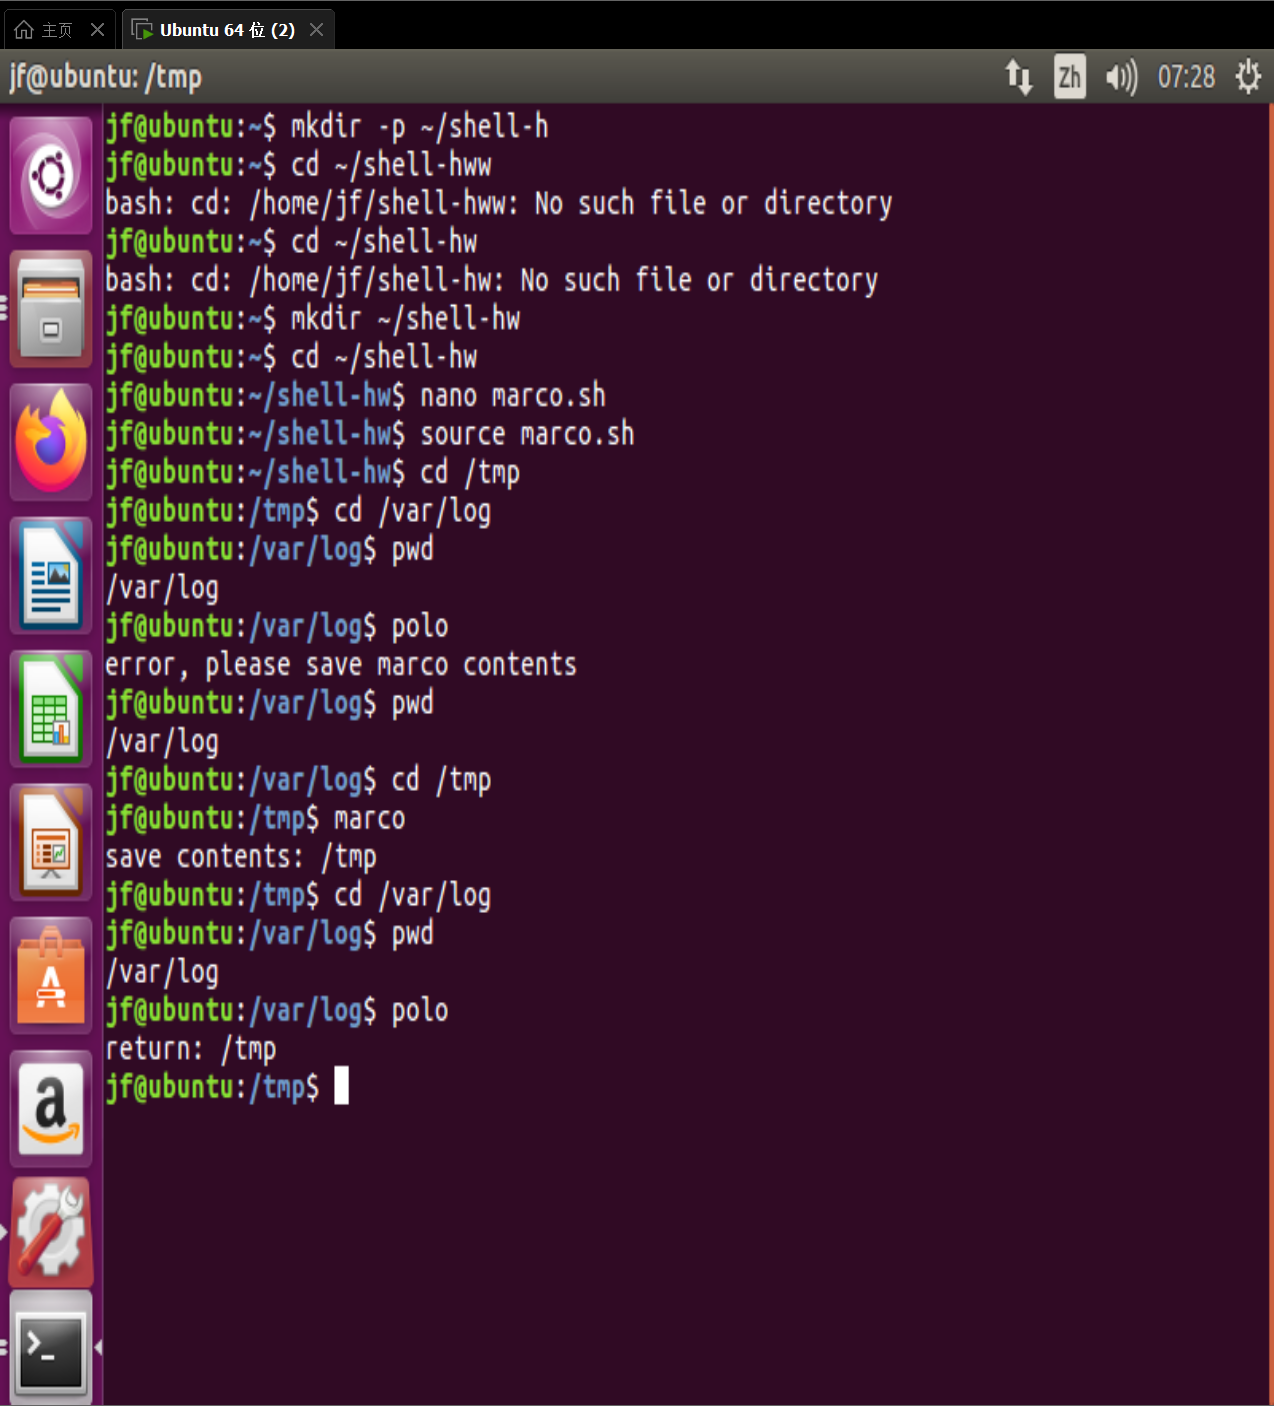
\includegraphics[width=0.9\textwidth]{marco_run.png}
    \caption{marco 保存 /tmp 目录，切到 /var/log 后 polo 成功返回 /tmp}
    \label{fig:marco_run}
\end{figure}

\subsubsection*{小结}
marco 把当前目录存入环境变量 MARCO\_DIR，polo 判断该变量非空后 cd 回去；未先 marco 直接 polo 会输出错误提示。通过 source 加载脚本即可在当前 shell 中使用这两个函数。

% ==================== 练习 3：alias dc ====================
\subsection{Aliases 与 Dotfiles：创建 alias dc}

\textbf{题目}：创建一个 alias dc，让你把 cd 打错时也能正常工作。

\begin{figure}[H]
    \centering
    
\includegraphics[width=0.9\textwidth]{alias_question.png}
    \caption{练习题目要求}
    \label{fig:alias_question}
\end{figure}

\subsubsection*{作答过程与运行结果}

\begin{lstlisting}[language=bash, caption={定义并使用别名 dc}]
$ alias dc='cd'
$ dc /tmp
$ nano ~/.bashrc       # 把 alias dc='cd' 写入配置文件永久生效
$ source ~/.bashrc
$ type dc
dc is aliased to `cd'
\end{lstlisting}

\begin{figure}[H]
    \centering
    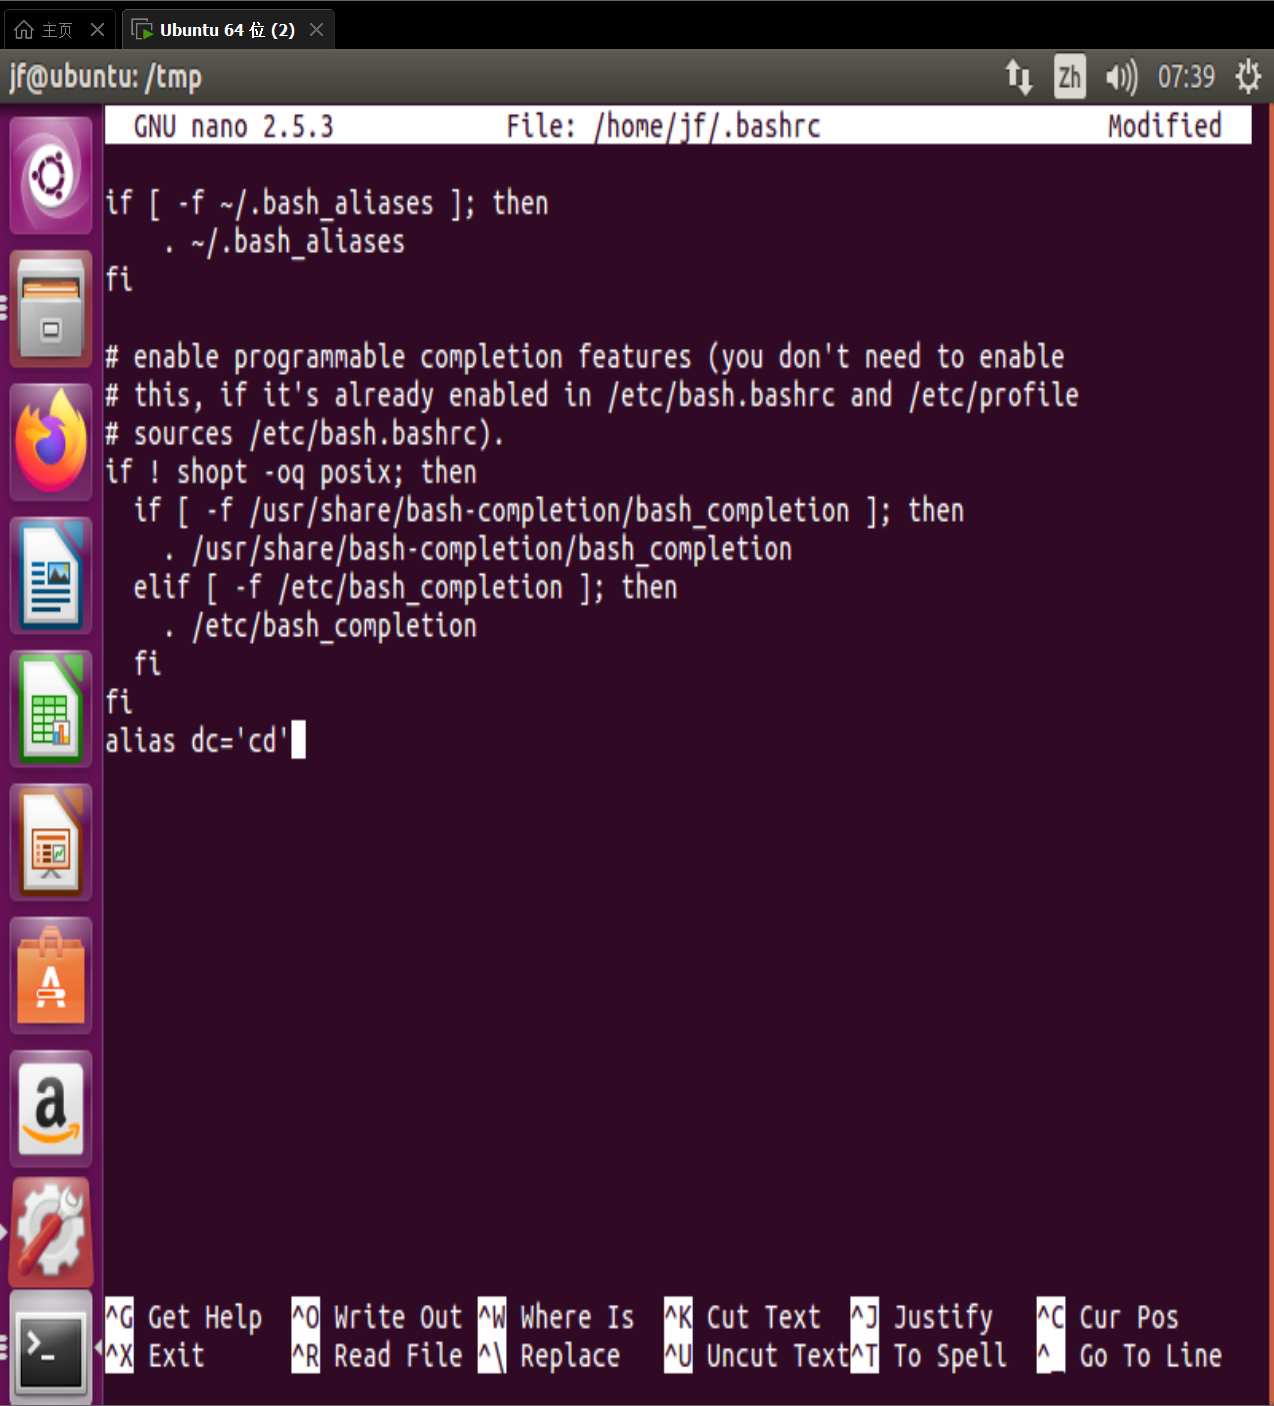
\includegraphics[width=0.9\textwidth]{alias_rc.png}
    \caption{在 .bashrc 中新增 alias dc='cd' 使其持久化}
    \label{fig:alias_rc}
\end{figure}

\begin{figure}[H]
    \centering
    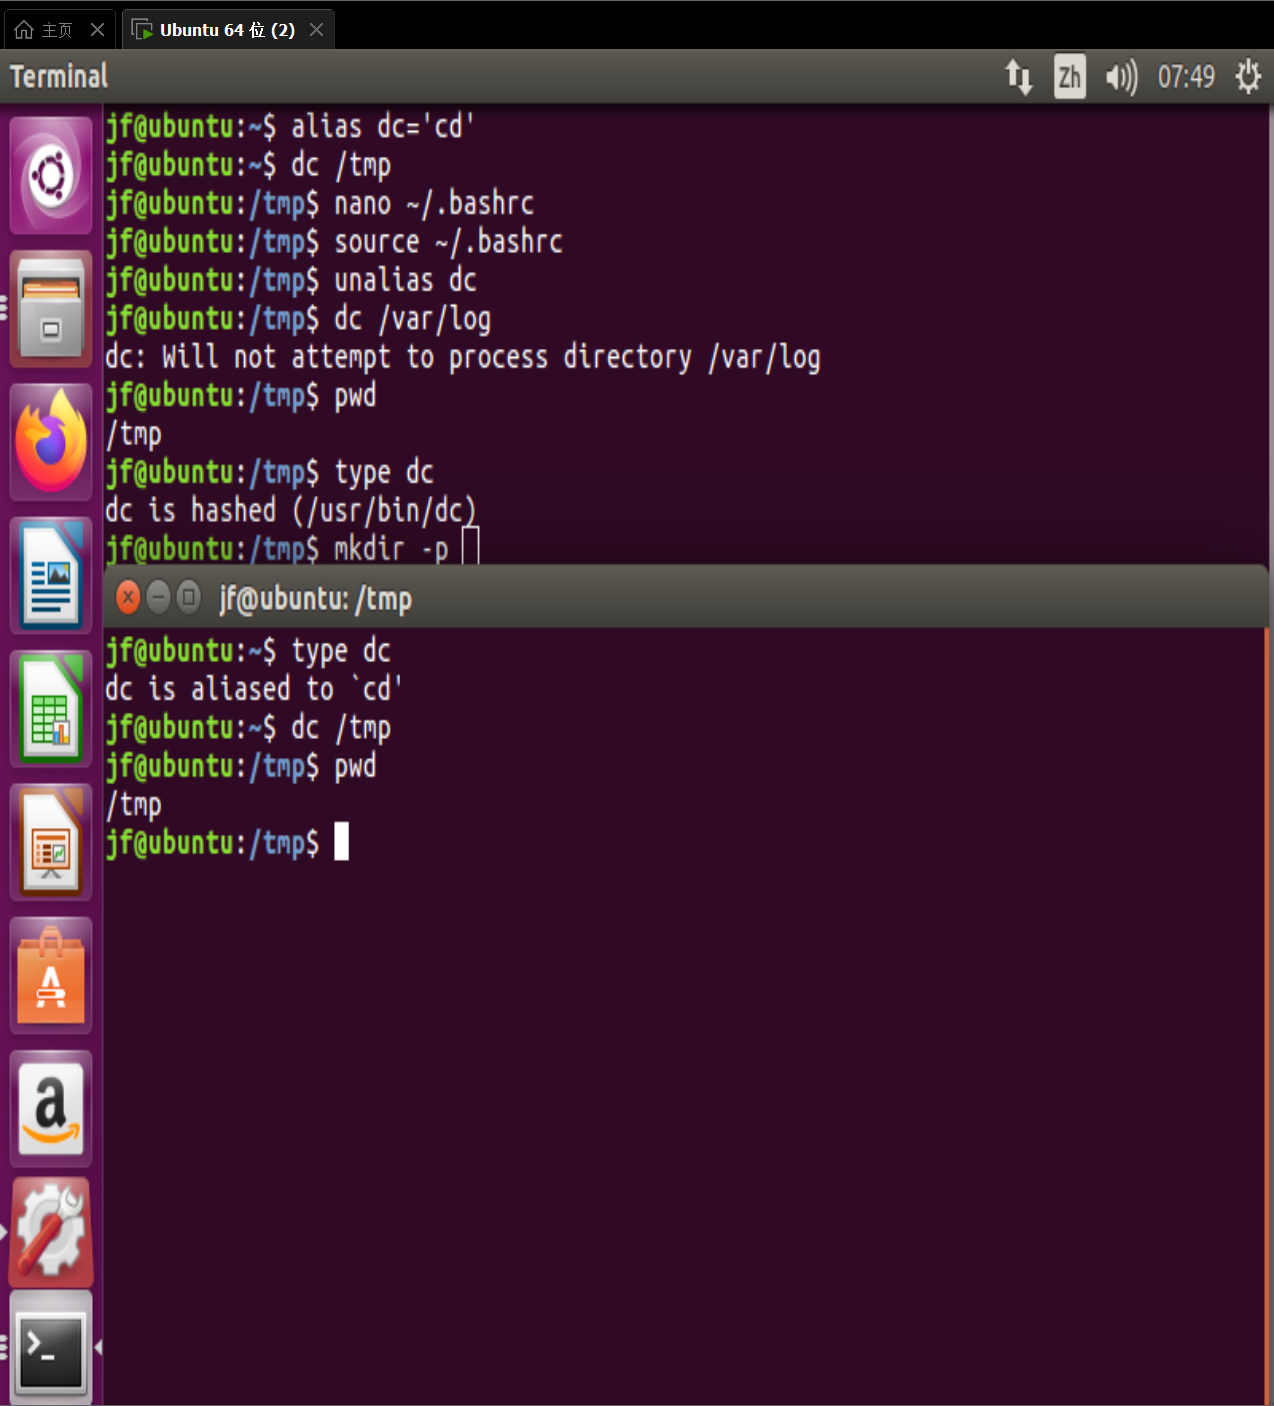
\includegraphics[width=0.9\textwidth]{alias_run.png}
    \caption{定义别名后 dc /tmp 正常切换；unalias 后 dc 恢复为系统命令}
    \label{fig:alias_run}
\end{figure}

\subsubsection*{小结}
alias dc='cd' 让"把 cd 打错成 dc"时也能正常切换目录；写入 .bashrc 并用 source 加载后永久生效；unalias 可临时取消别名（此时 dc 恢复为 /usr/bin/dc）。

% ==================== 练习 4：ls 命令 ====================
\subsection{阅读 man ls，组合 ls 命令}

\textbf{题目}：阅读 man ls，写出一个 ls 命令，让它按下面的方式列出文件：包含所有文件（包括隐藏文件）、文件大小以易读格式显示（例如 454M）、按最近修改时间排序、输出带颜色。

\begin{figure}[H]
    \centering
    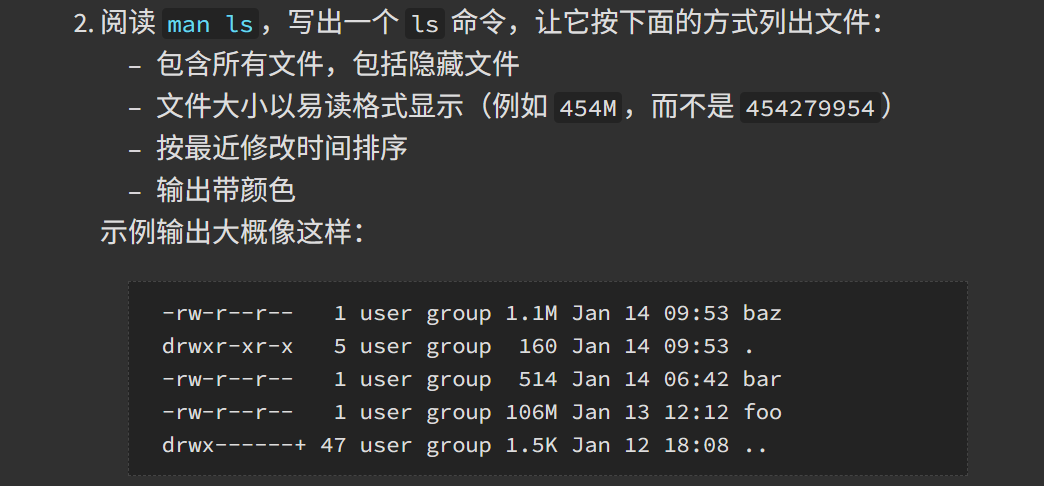
\includegraphics[width=0.9\textwidth]{ls_question.png}
    \caption{练习题目要求}
    \label{fig:ls_question}
\end{figure}

\subsubsection*{作答过程与运行结果}

组合各选项得到命令 \texttt{ls -alht --color=auto}：

\begin{lstlisting}[language=bash, caption={组合 ls 选项}]
$ ls -alht --color=auto
# -a  包含隐藏文件（含 . 与 ..）
# -l  长格式（权限、属主、大小、时间）
# -h  大小以易读格式显示（4.0K / 4.1K 等）
# -t  按最近修改时间排序（最新在前）
# --color=auto  输出带颜色
\end{lstlisting}

\begin{figure}[H]
    \centering
    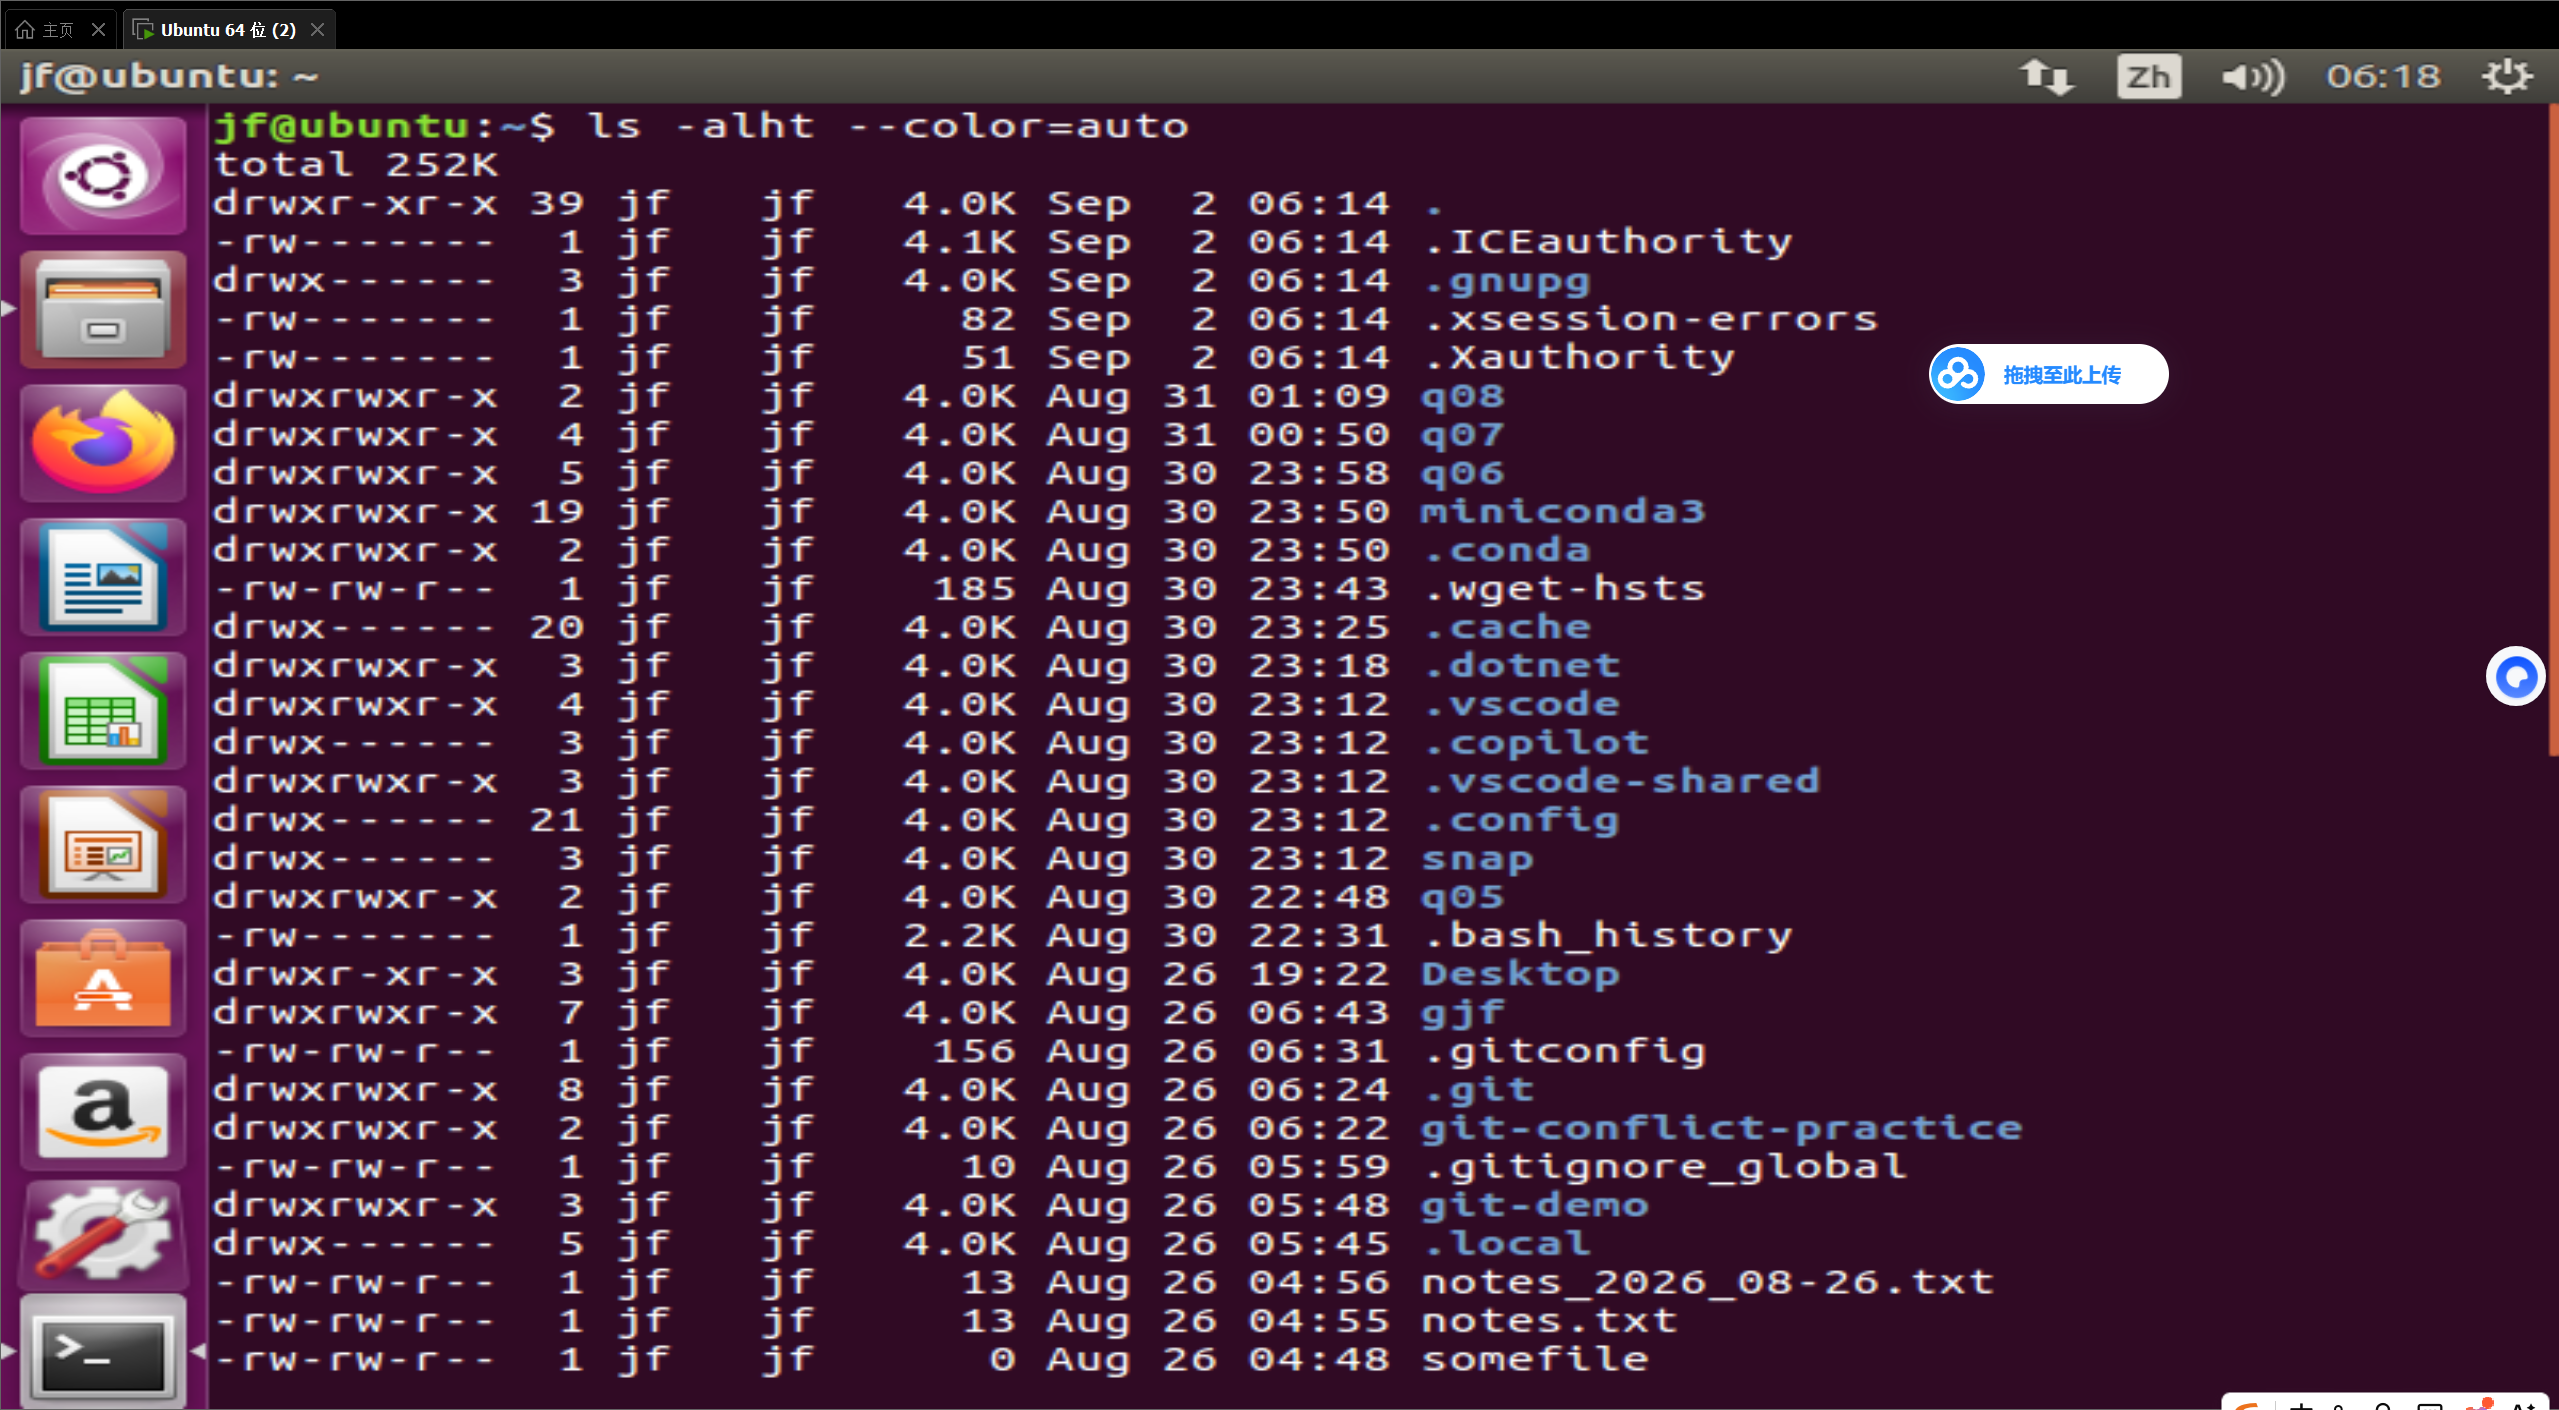
\includegraphics[width=0.9\textwidth]{ls_run1.png}
    \caption{ls -alht --color=auto 输出（含隐藏文件、易读大小、时间排序、彩色）}
    \label{fig:ls_run1}
\end{figure}

\begin{figure}[H]
    \centering
    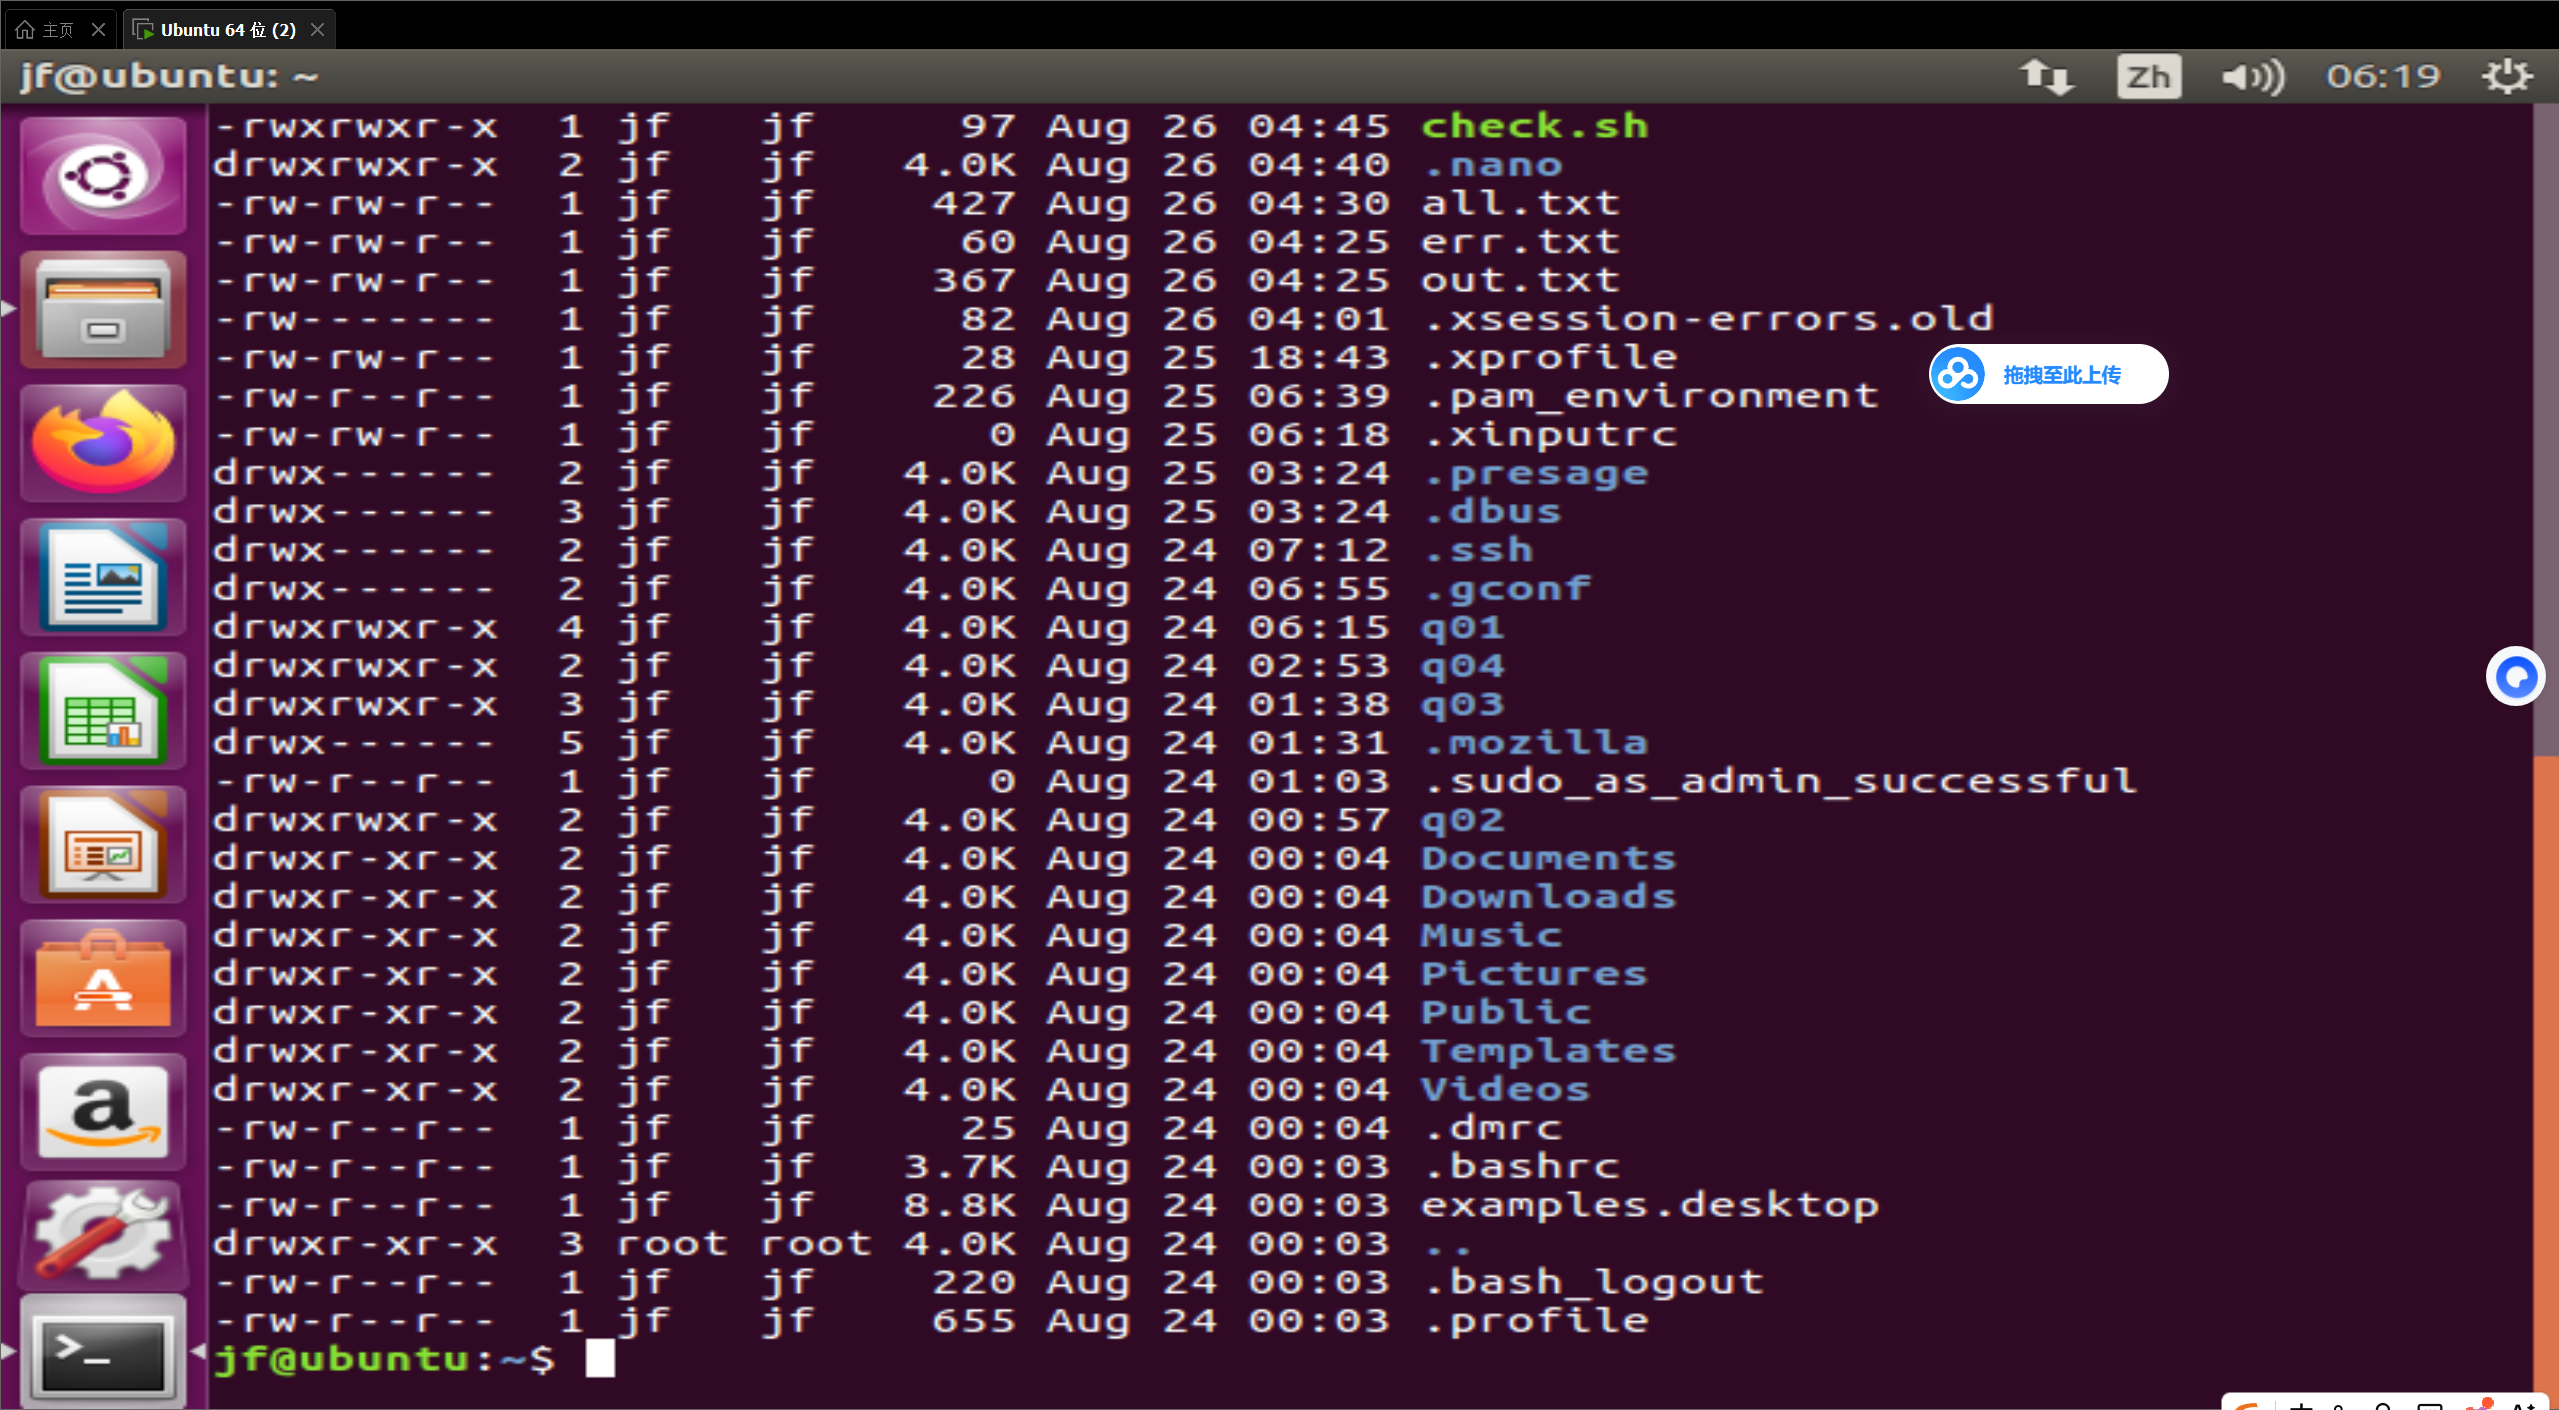
\includegraphics[width=0.9\textwidth]{ls_run2.png}
    \caption{另一目录下的 ls -alht 输出}
    \label{fig:ls_run2}
\end{figure}

\subsubsection*{小结}
通过 man ls 查阅各选项含义后组合出 ls -alht --color=auto，同时满足"包含隐藏文件、易读大小、按修改时间排序、带颜色"四个要求。

% ==================== 练习 5：-- 特殊参数 ====================
\subsection{\texttt{-{}-} 特殊参数}

\textbf{题目}：你可能见过像 cmd --flag -- --notaflag 这样的命令。这里的 -- 是一个特殊参数，它告诉程序后面不要再继续解析选项（flag）了。也就是说，-- 后面的所有内容都会被当作位置参数（positional argument）。这有什么用？试着运行 touch -- -myfile，然后在不使用 -- 的情况下把它删掉。

\begin{figure}[H]
    \centering
    
\includegraphics[width=0.9\textwidth]{dash_question.png}
    \caption{练习题目要求}
    \label{fig:dash_question}
\end{figure}

\subsubsection*{作答过程与运行结果}

\begin{lstlisting}[language=bash, caption={用 -- 创建以 - 开头的文件并删除}]
$ touch -- -myfile          # 创建名为 -myfile 的文件
$ ls -l
-rw-rw-r-- 1 jf jf 0 Sep 2 19:14 -myfile
$ rm -myfile                # 不使用 -- 直接删除：报错
rm: invalid option -- 'm'
Try 'rm ./-myfile' to remove the file '-myfile'.
$ rm ./-myfile              # 用 ./ 前缀指明路径后成功删除
\end{lstlisting}

\begin{figure}[H]
    \centering
    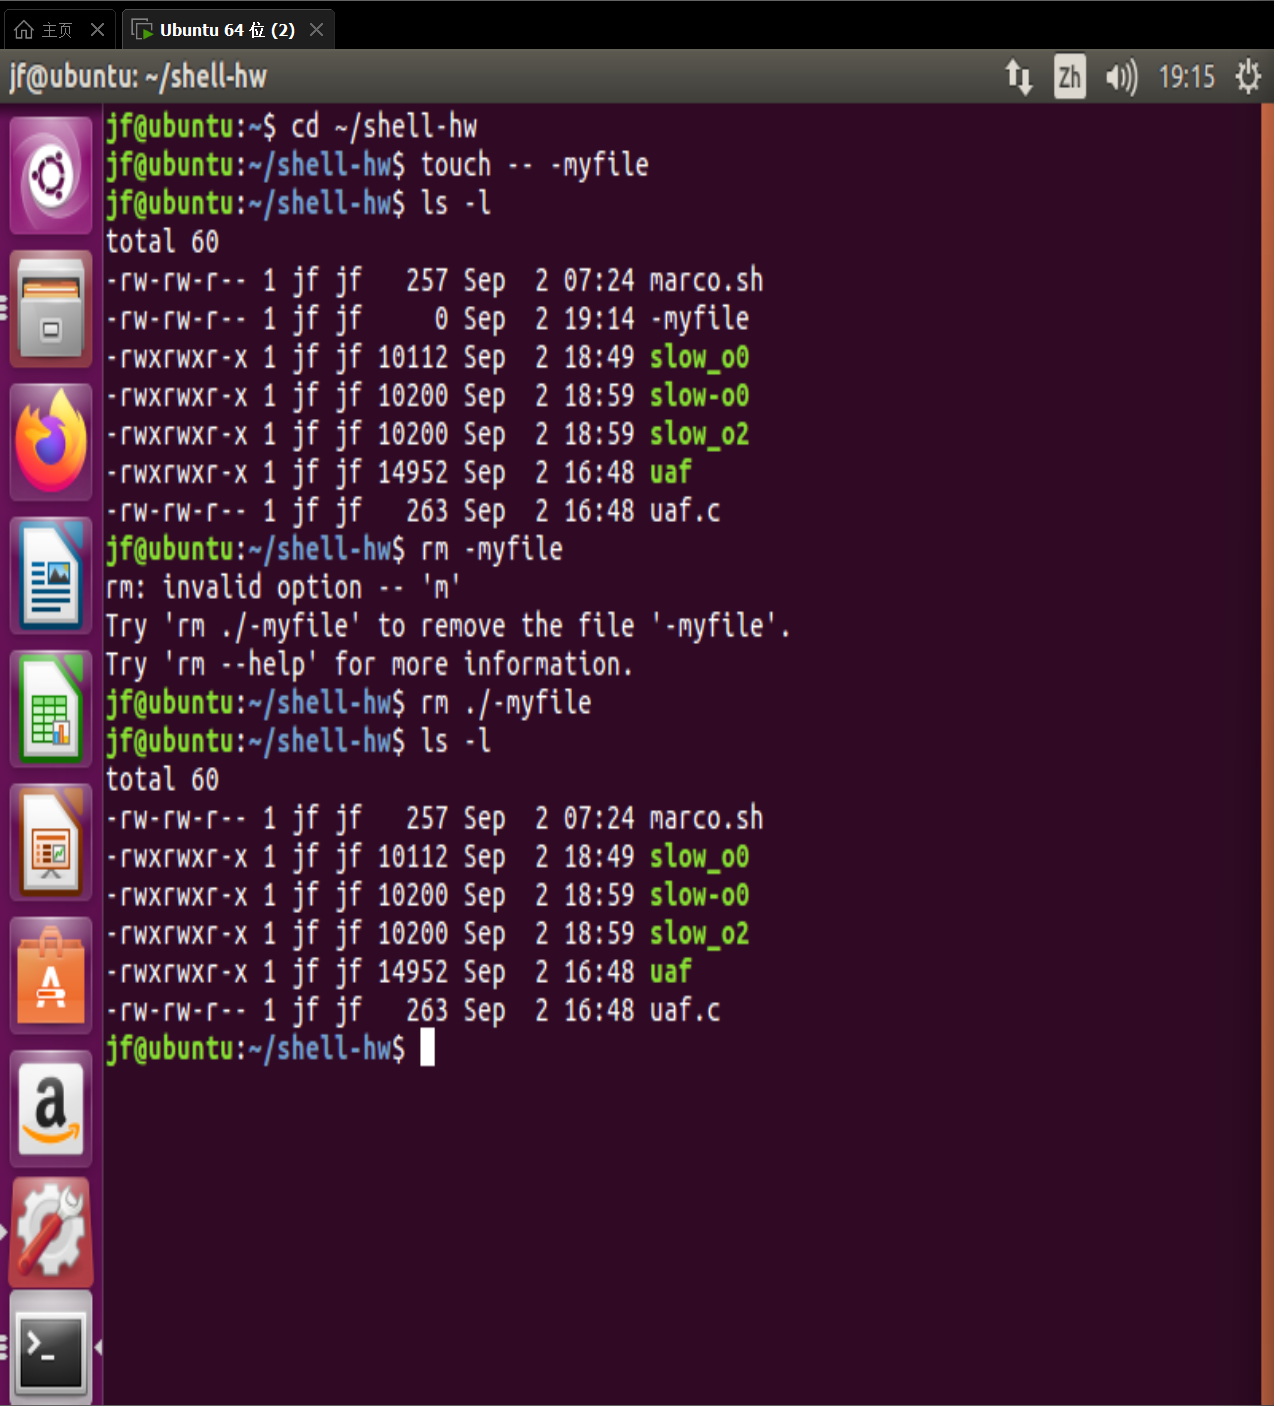
\includegraphics[width=0.9\textwidth]{dash_run.png}
    \caption{touch -- -myfile 创建文件，rm -myfile 报错，rm ./-myfile 成功}
    \label{fig:dash_run}
\end{figure}

\subsubsection*{小结}
-- 告诉程序后面的内容按位置参数处理，因此 touch -- -myfile 能创建以 - 开头的文件；删除时若不使用 -- 会被 rm 误认为选项而报错，改用 ./ 前缀（rm ./-myfile）同样可以解决问题。

% ==================== 练习 6：strace ====================
\subsection{用 strace 追踪系统调用}

\textbf{题目}：Use strace (Linux) or dtruss (macOS) to trace the system calls made by a command like ls -l. What system calls is it making? Try tracing a more complex program and see what files it opens.

\begin{figure}[H]
    \centering
    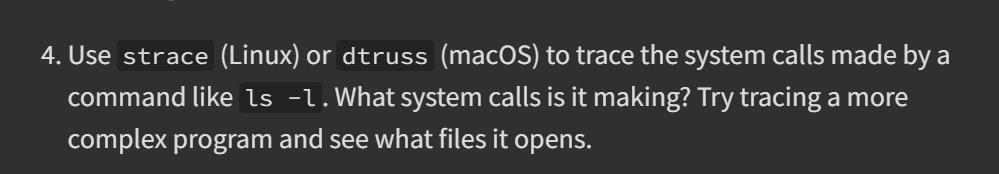
\includegraphics[width=0.9\textwidth]{strace_question.png}
    \caption{练习题目要求}
    \label{fig:strace_question}
\end{figure}

\subsubsection*{作答过程与运行结果}

\begin{lstlisting}[language=bash, caption={追踪 ls -l 的系统调用}]
$ strace ls -l
execve("/bin/ls", ["ls", "-l"], [/* 65 vars */]) = 0
brk(NULL) = 0xed1000
access("/etc/ld.so.nohwcap", F_OK) = -1 ENOENT
open("/etc/ld.so.cache", O_RDONLY|O_CLOEXEC) = 3
mmap(NULL, 91144, PROT_READ, MAP_PRIVATE, 3, 0) = 0x7facd075d000
...
\end{lstlisting}

\begin{figure}[H]
    \centering
    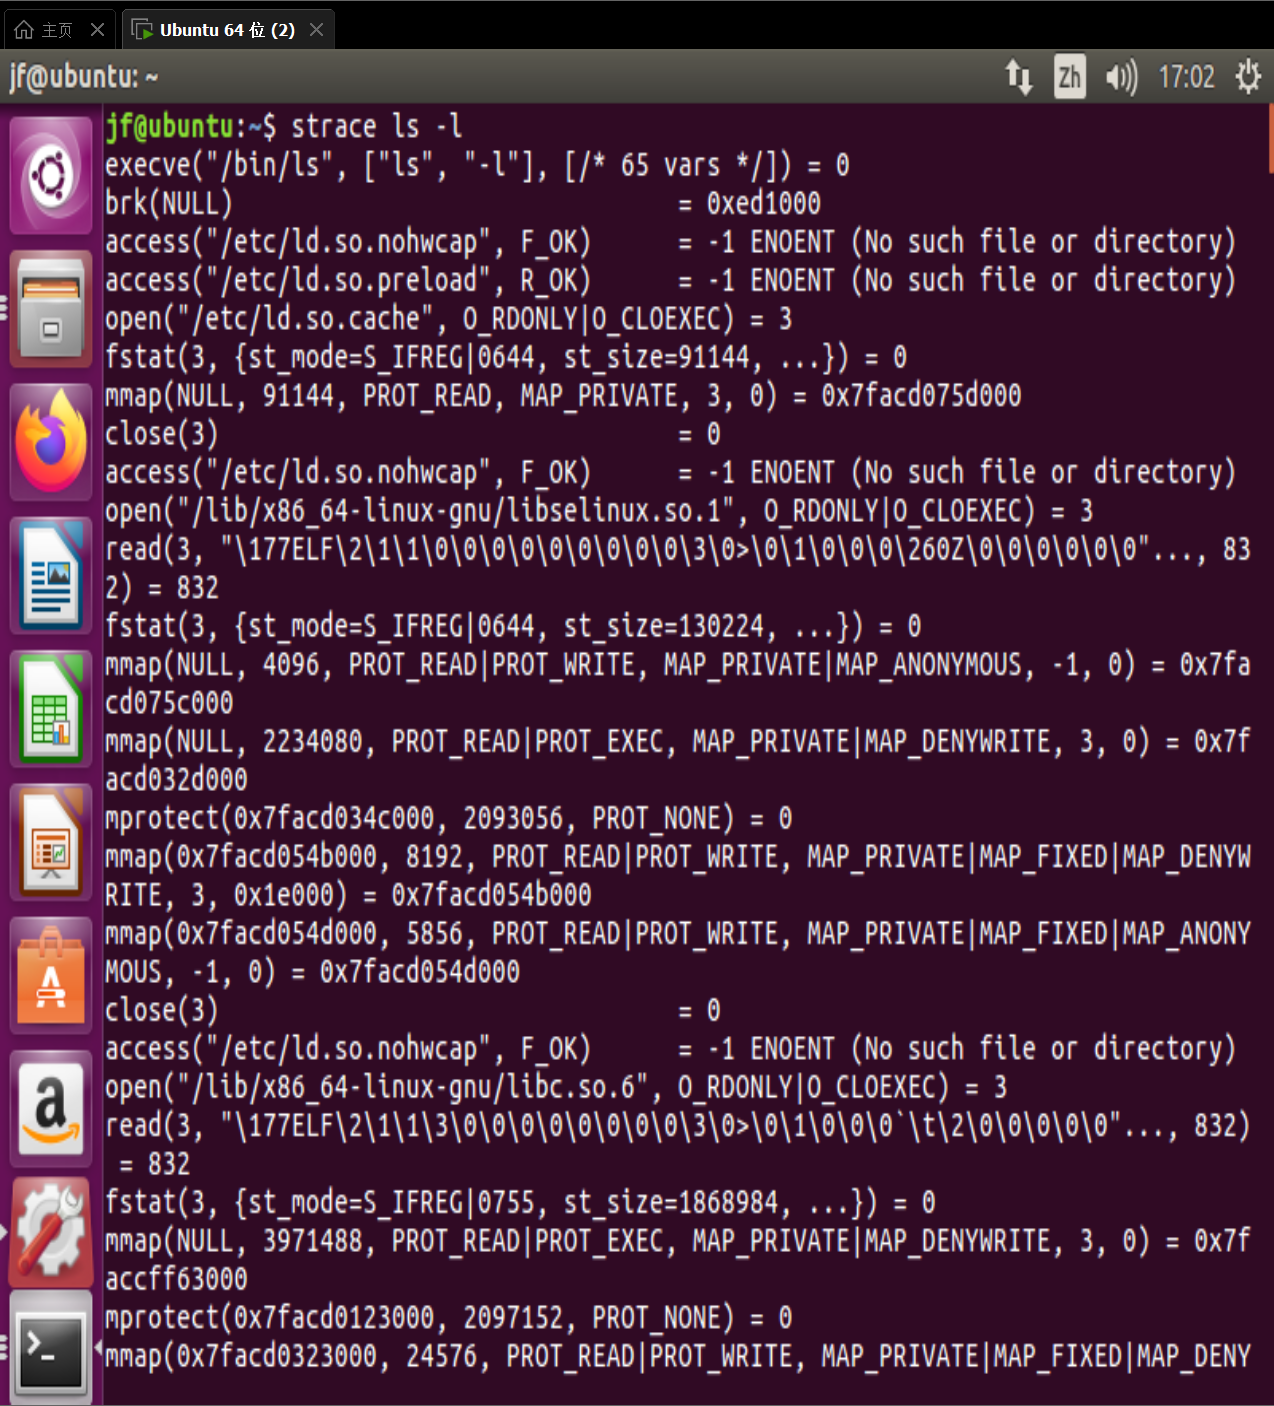
\includegraphics[width=0.9\textwidth]{strace_run1.png}
    \caption{strace ls -l：加载动态库等系统调用序列}
    \label{fig:strace_run1}
\end{figure}

\begin{figure}[H]
    \centering
    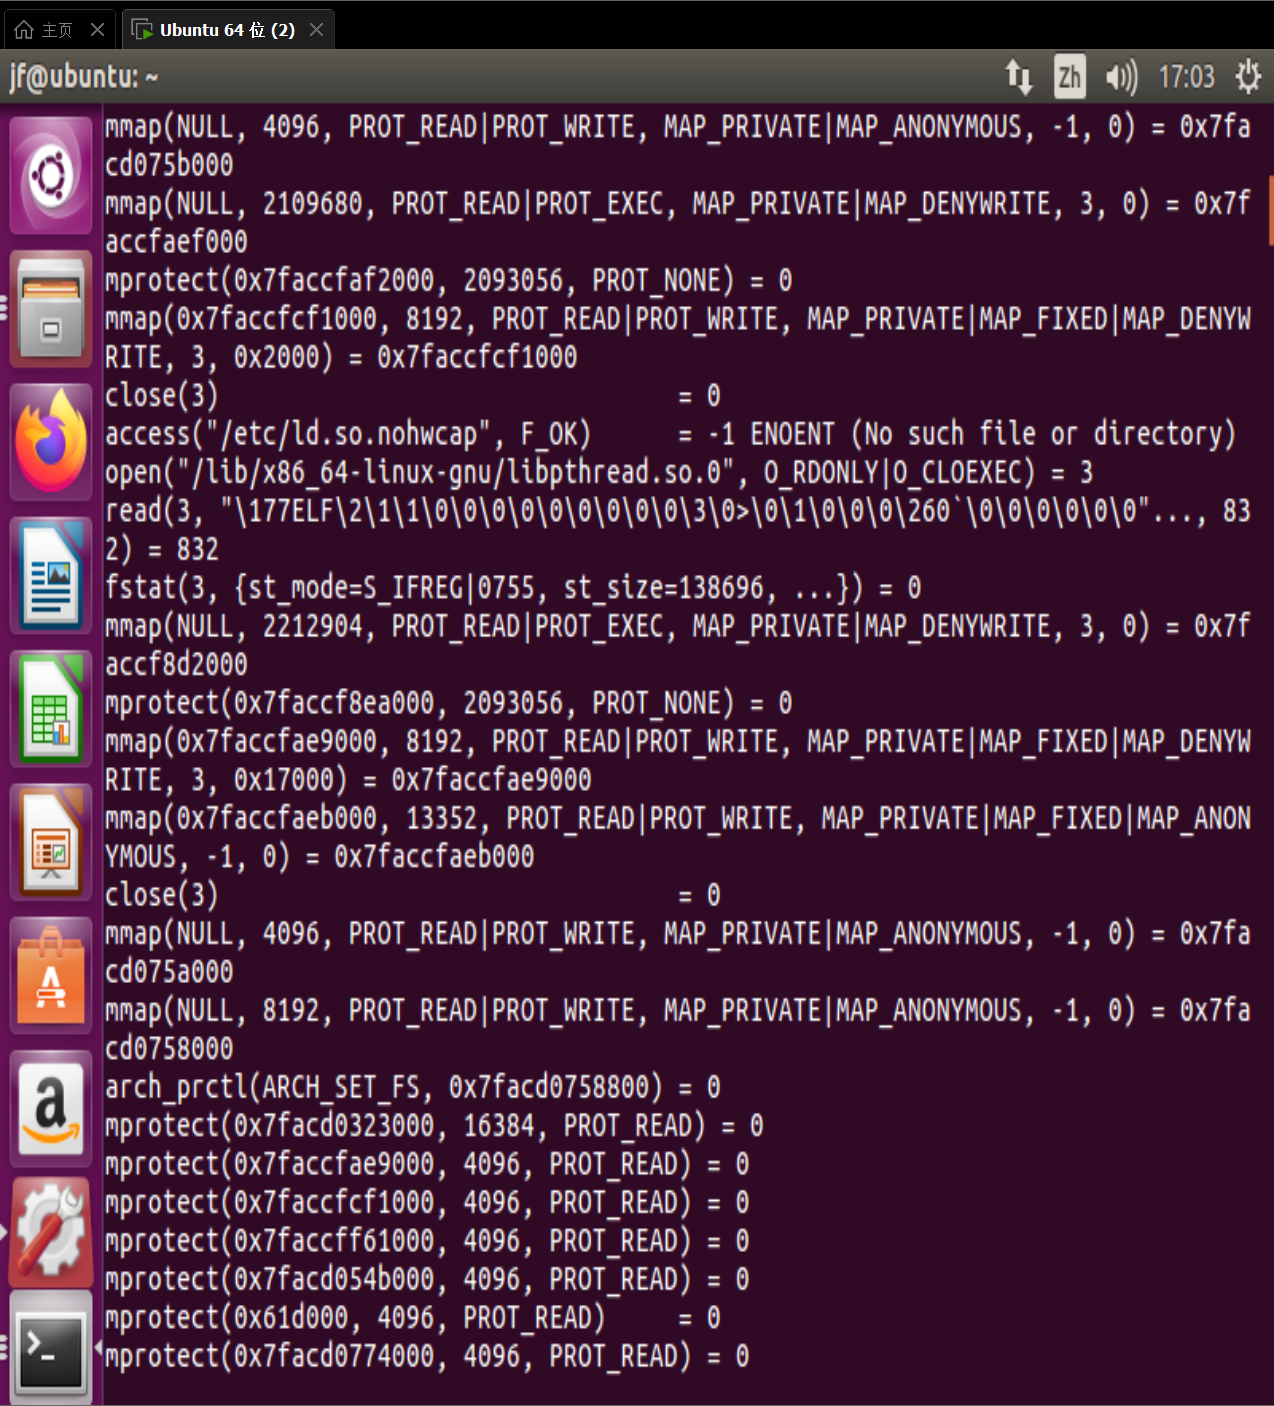
\includegraphics[width=0.9\textwidth]{strace_run2.png}
    \caption{strace ls -l 后续输出（mmap/mprotect/close 等）}
    \label{fig:strace_run2}
\end{figure}

只追踪文件相关的系统调用，并统计各类系统调用次数：

\begin{lstlisting}[language=bash, caption={按类别追踪与统计}]
$ strace -e trace=file ls -l        # 只显示文件相关调用
$ strace -c ls -l                   # 统计各类系统调用次数与耗时
% time seconds usecs/call calls errors syscall
0.00 0.000000 0 17 read
0.00 0.000000 0 31 write
0.00 0.000000 0 27 5 open
...
0.00 0.000000 0 52 52 getxattr
0.00 0.000000 0 30 30 lgetxattr
\end{lstlisting}

\begin{figure}[H]
    \centering
    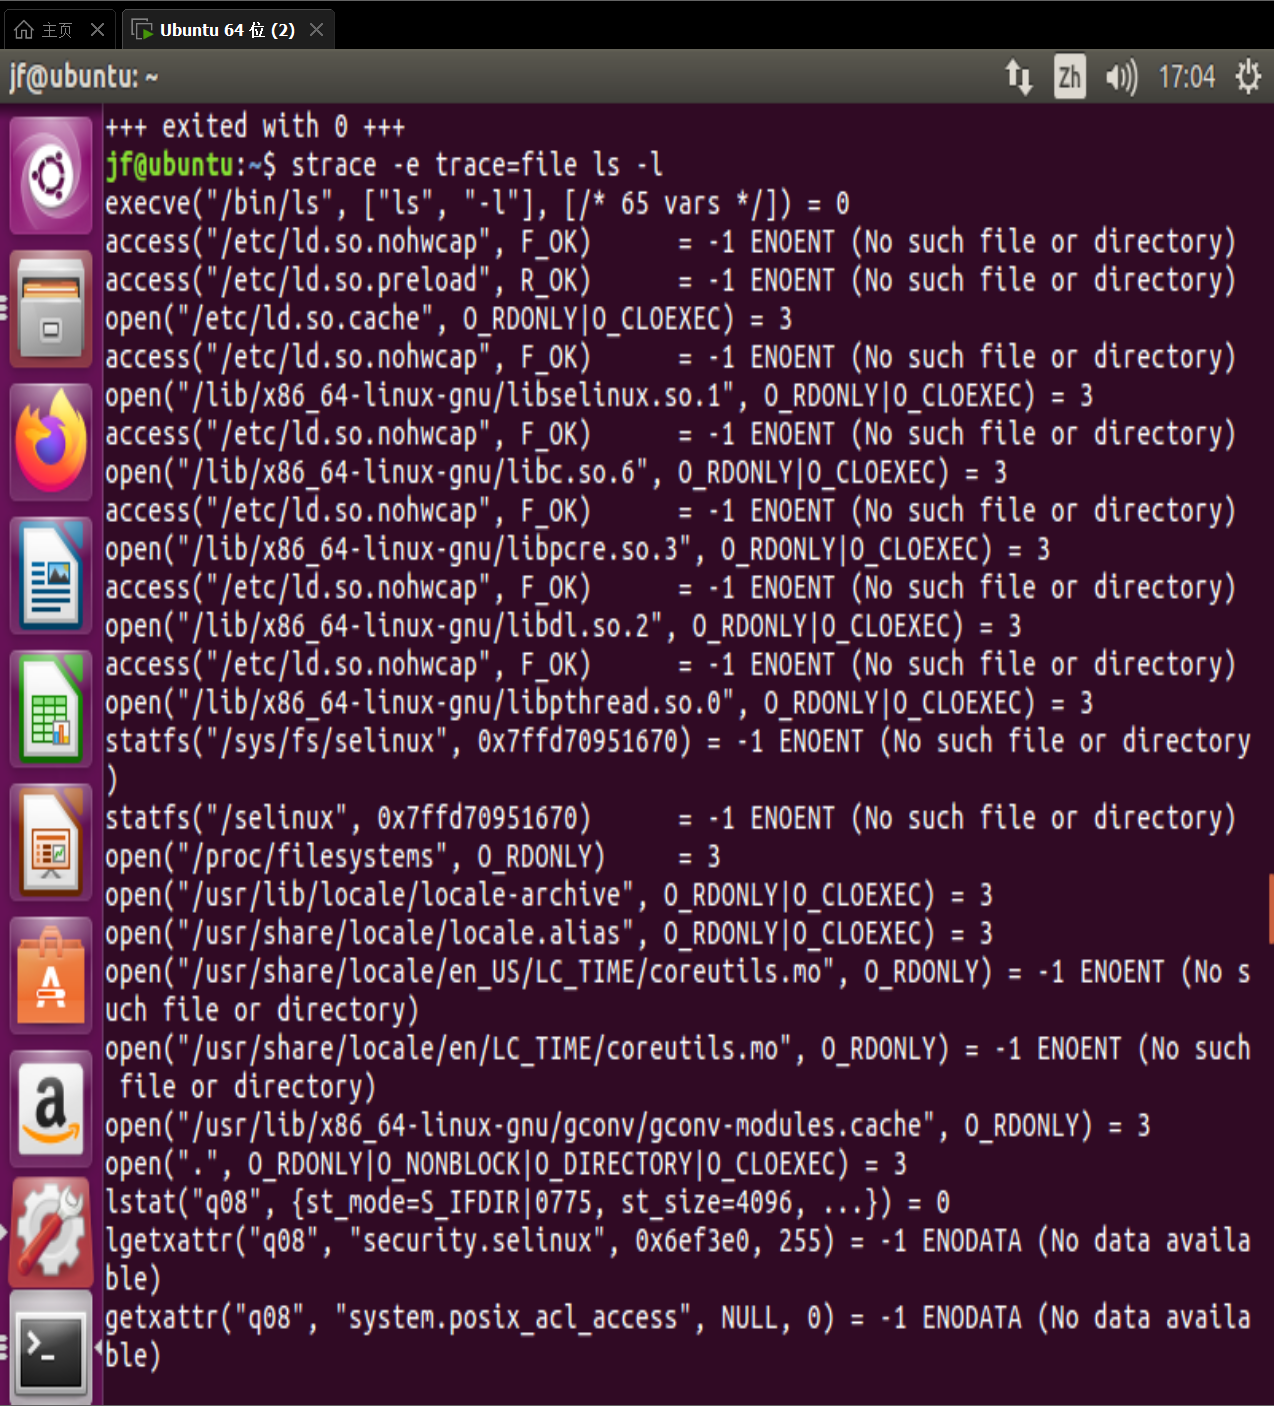
\includegraphics[width=0.9\textwidth]{strace_file.png}
    \caption{strace -e trace=file ls -l：仅显示文件相关系统调用}
    \label{fig:strace_file}
\end{figure}

\begin{figure}[H]
    \centering
    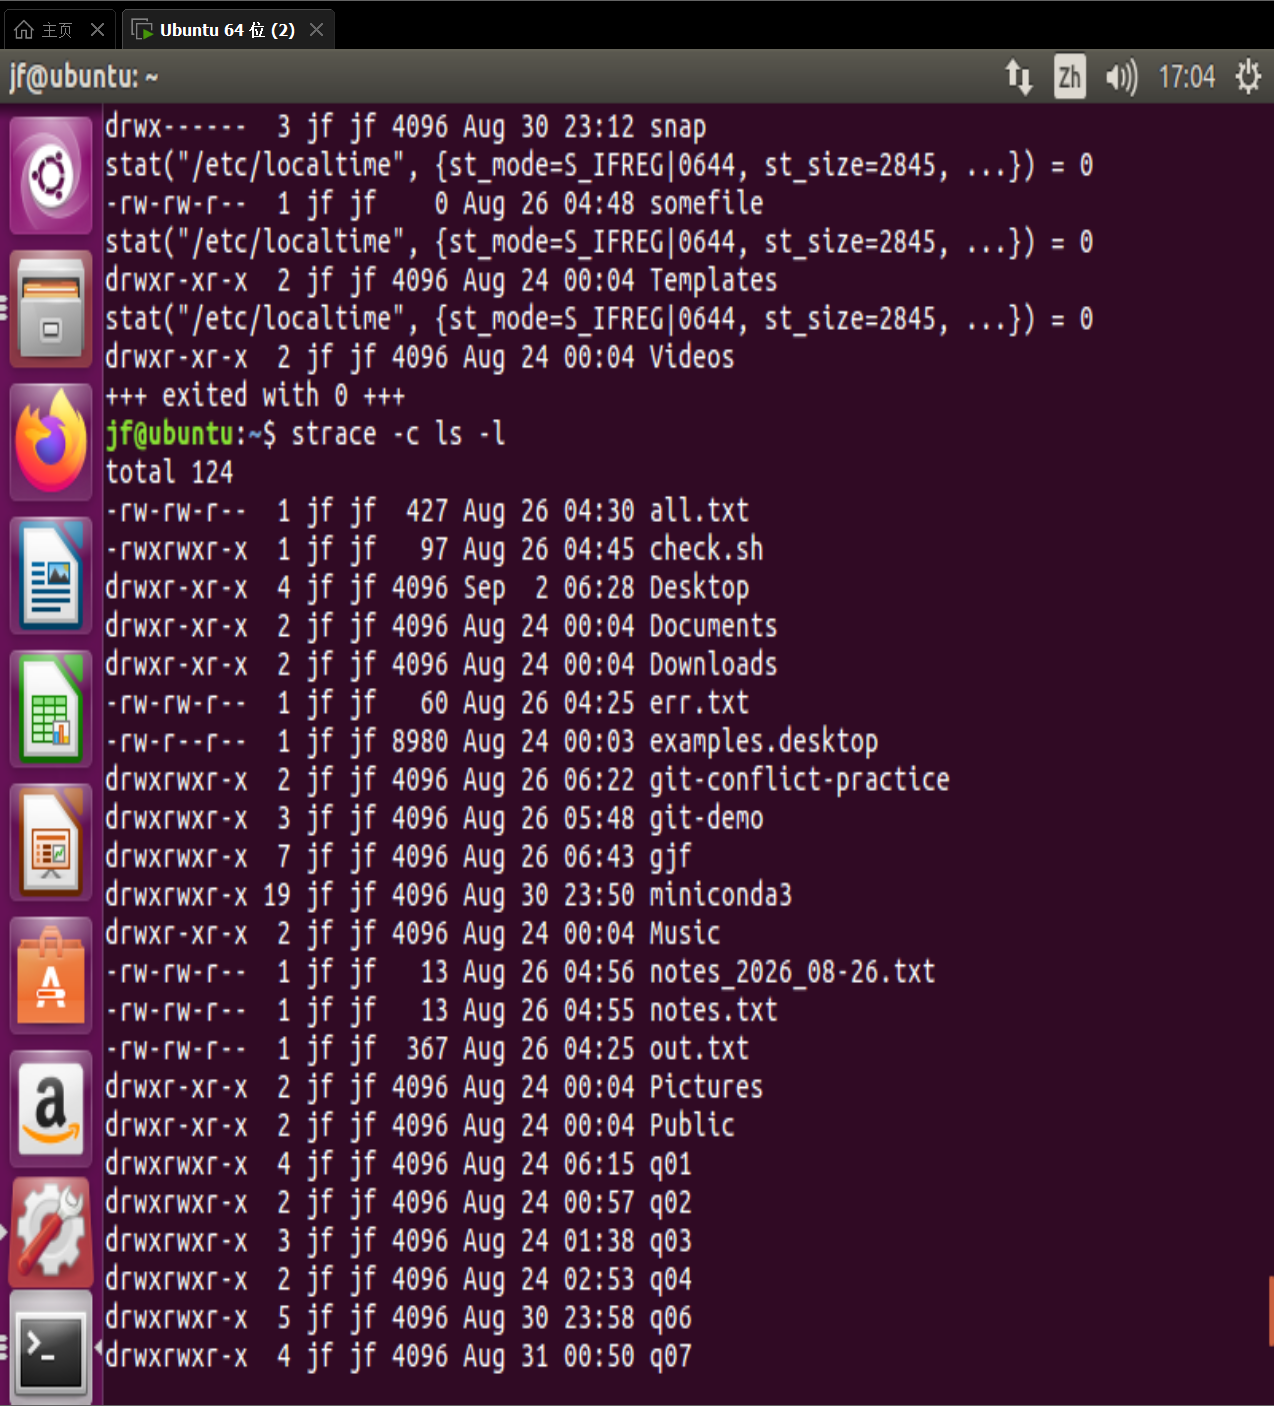
\includegraphics[width=0.9\textwidth]{strace_c1.png}
    \caption{strace -c ls -l：输出文件列表并统计调用}
    \label{fig:strace_c1}
\end{figure}

\begin{figure}[H]
    \centering
    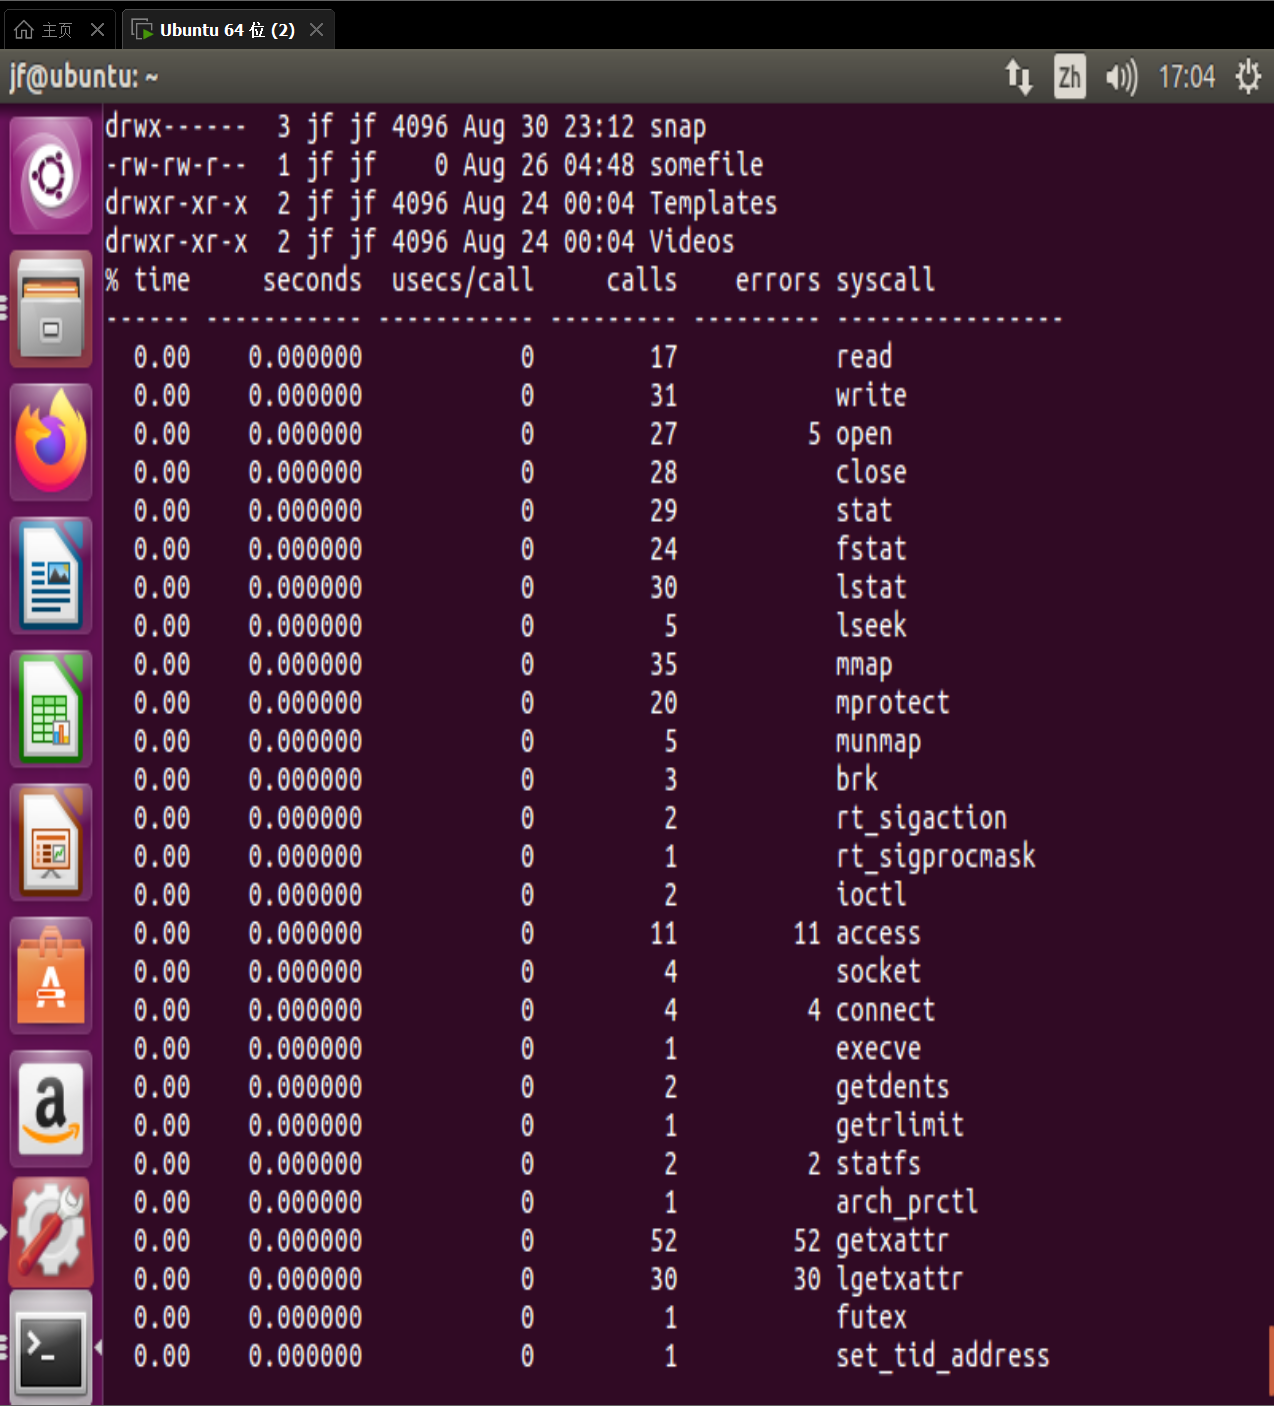
\includegraphics[width=0.9\textwidth]{strace_c2.png}
    \caption{strace -c 统计表：read/write/open/getxattr 等系统调用次数}
    \label{fig:strace_c2}
\end{figure}

\subsubsection*{小结}
strace 能列出命令执行时向内核发起的每一次系统调用。ls -l 会先 execve 启动自身，加载动态库（open/mmap 共享库），再 open 目录、用 lstat/lgetxattr 读取每个文件元数据；strace -c 还能给出各类调用的次数统计，帮助理解程序的底层行为。

% ==================== 练习 7：AddressSanitizer ====================
\subsection{用 AddressSanitizer 调试内存错误}

\textbf{题目}：Debug a memory error with AddressSanitizer. Save this as uaf.c：先分配 32 字节内存并拷贝字符串打印，释放后又修改已释放内存的内容并打印。先不带消毒器编译运行（可能正常），再用 -fsanitize=address 编译运行，阅读错误报告，找出 ASan 检测到的 bug 并修复。

\begin{figure}[H]
    \centering
    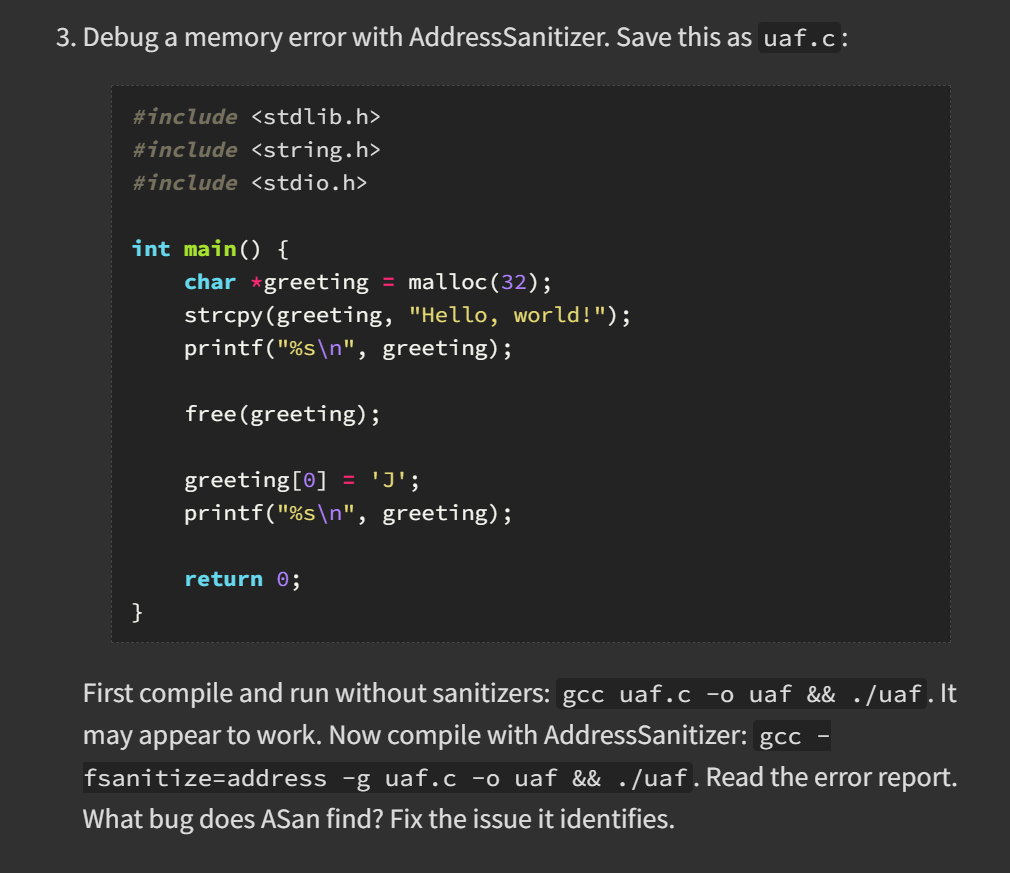
\includegraphics[width=0.9\textwidth]{asan_question.png}
    \caption{练习题目要求}
    \label{fig:asan_question}
\end{figure}

\subsubsection*{作答过程与运行结果}

\begin{lstlisting}[language=C, caption={uaf.c：释放后使用（use-after-free）}]
#include <stdlib.h>
#include <string.h>
#include <stdio.h>
int main() {
    char *greeting = malloc(32);
    strcpy(greeting, "Hello, world!");
    printf("%s\n", greeting);
    free(greeting);          // 释放
    greeting[0] = 'J';       // 释放后再写 —— use-after-free
    printf("%s\n", greeting);
    return 0;
}
\end{lstlisting}

\begin{figure}[H]
    \centering
    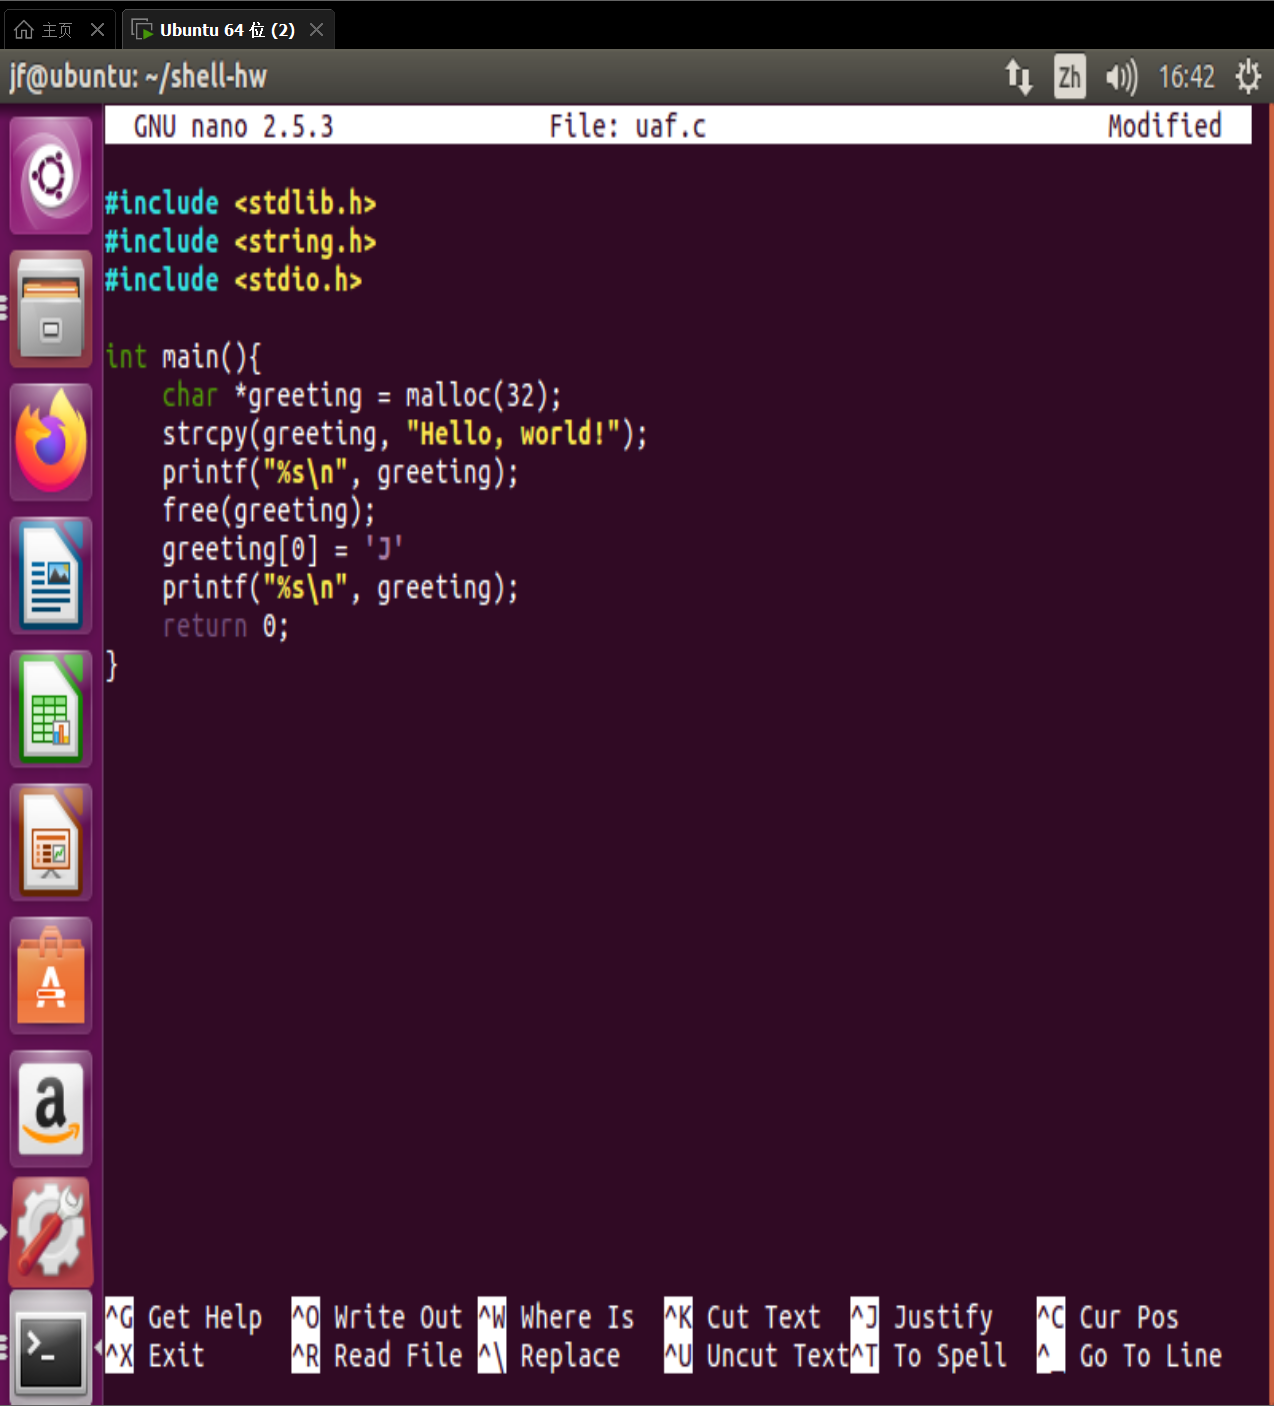
\includegraphics[width=0.9\textwidth]{asan_code.png}
    \caption{nano 中编辑 uaf.c（free 后又访问 greeting）}
    \label{fig:asan_code}
\end{figure}

\begin{lstlisting}[language=bash, caption={普通编译运行 + ASan 编译运行}]
$ gcc uaf.c -o uaf && ./uaf     # 不带消毒器：看似正常
Hello, world!
$ gcc -fsanitize=address -g uaf.c -o uaf && ./uaf
Hello, world!
==5073==ERROR: AddressSanitizer: heap-use-after-free on address 0x60300000efe0
WRITE of size 1 at 0x60300000efe0 thread T0
#0 0x40093d in main /home/jf/shell-hw/uaf.c:10
freed by thread T0 here:
#1 0x400909 in main /home/jf/shell-hw/uaf.c:9
previously allocated by thread T0 here:
#1 0x4008d7 in main /home/jf/shell-hw/uaf.c:6
SUMMARY: AddressSanitizer: heap-use-after-free /home/jf/shell-hw/uaf.c:10 main
==5073==ABORTING
\end{lstlisting}

\begin{figure}[H]
    \centering
    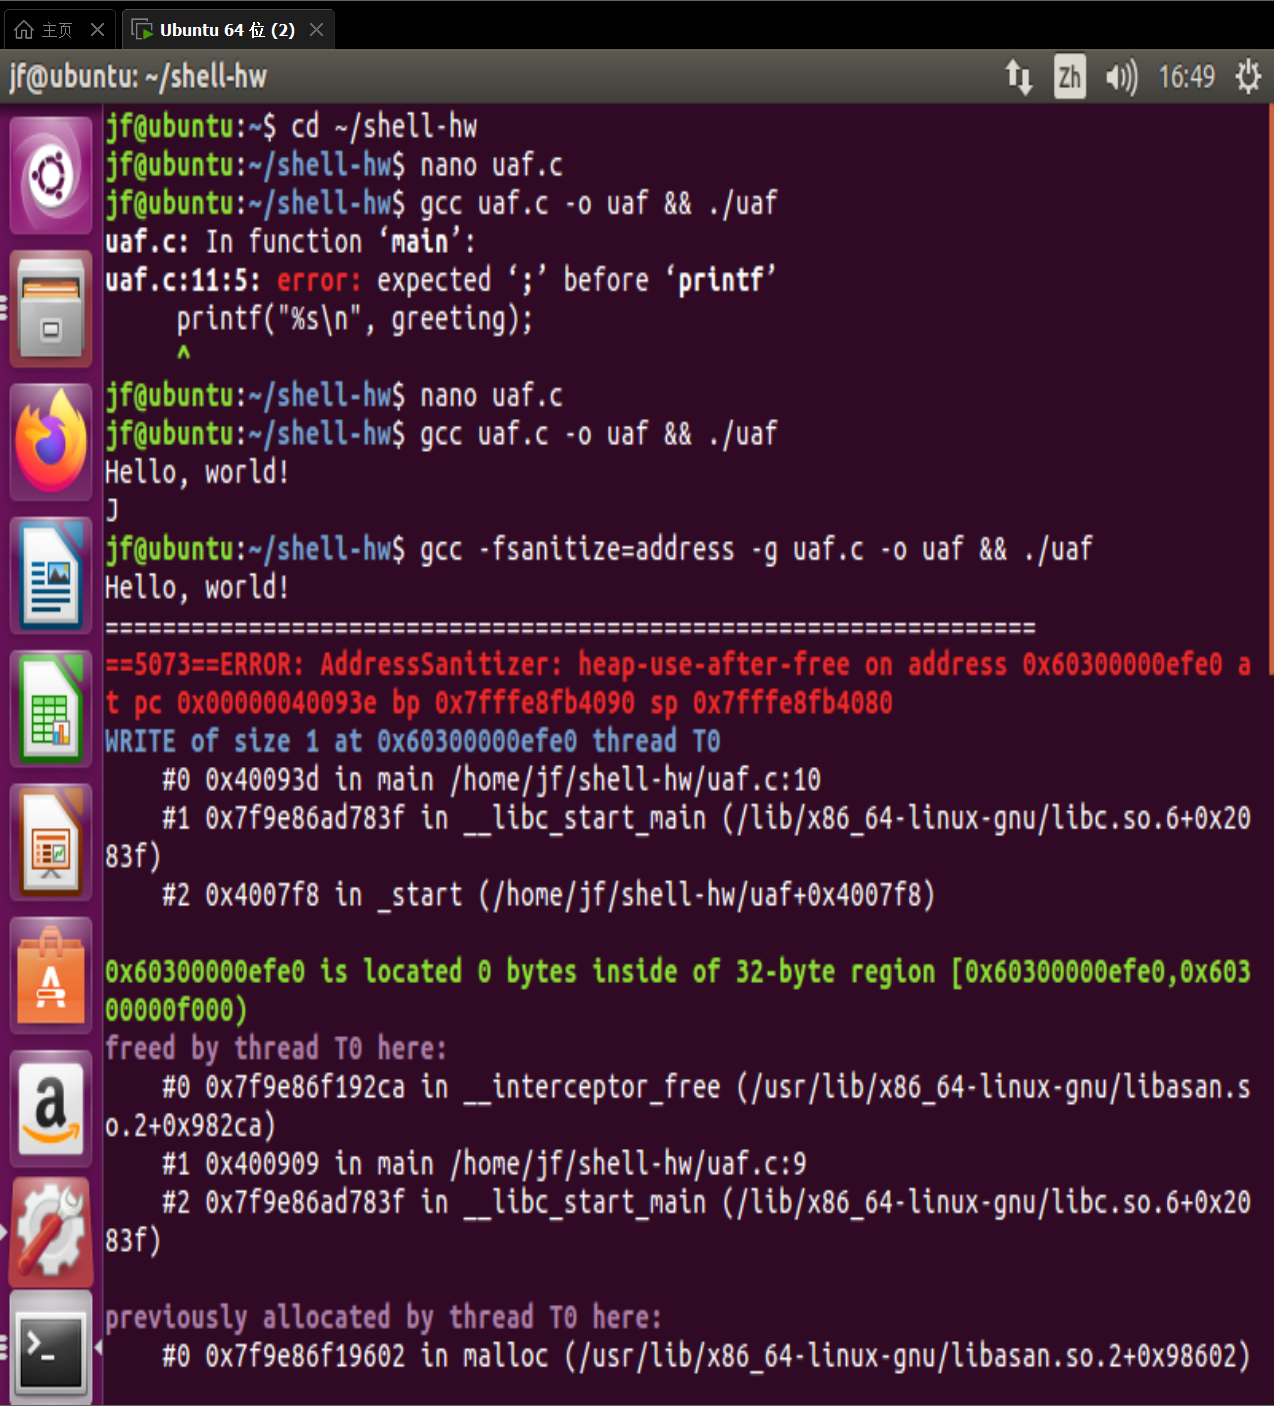
\includegraphics[width=0.9\textwidth]{asan_compile.png}
    \caption{首次编译报缺分号，修正后普通编译正常，ASan 检测到 use-after-free}
    \label{fig:asan_compile}
\end{figure}

\begin{figure}[H]
    \centering
    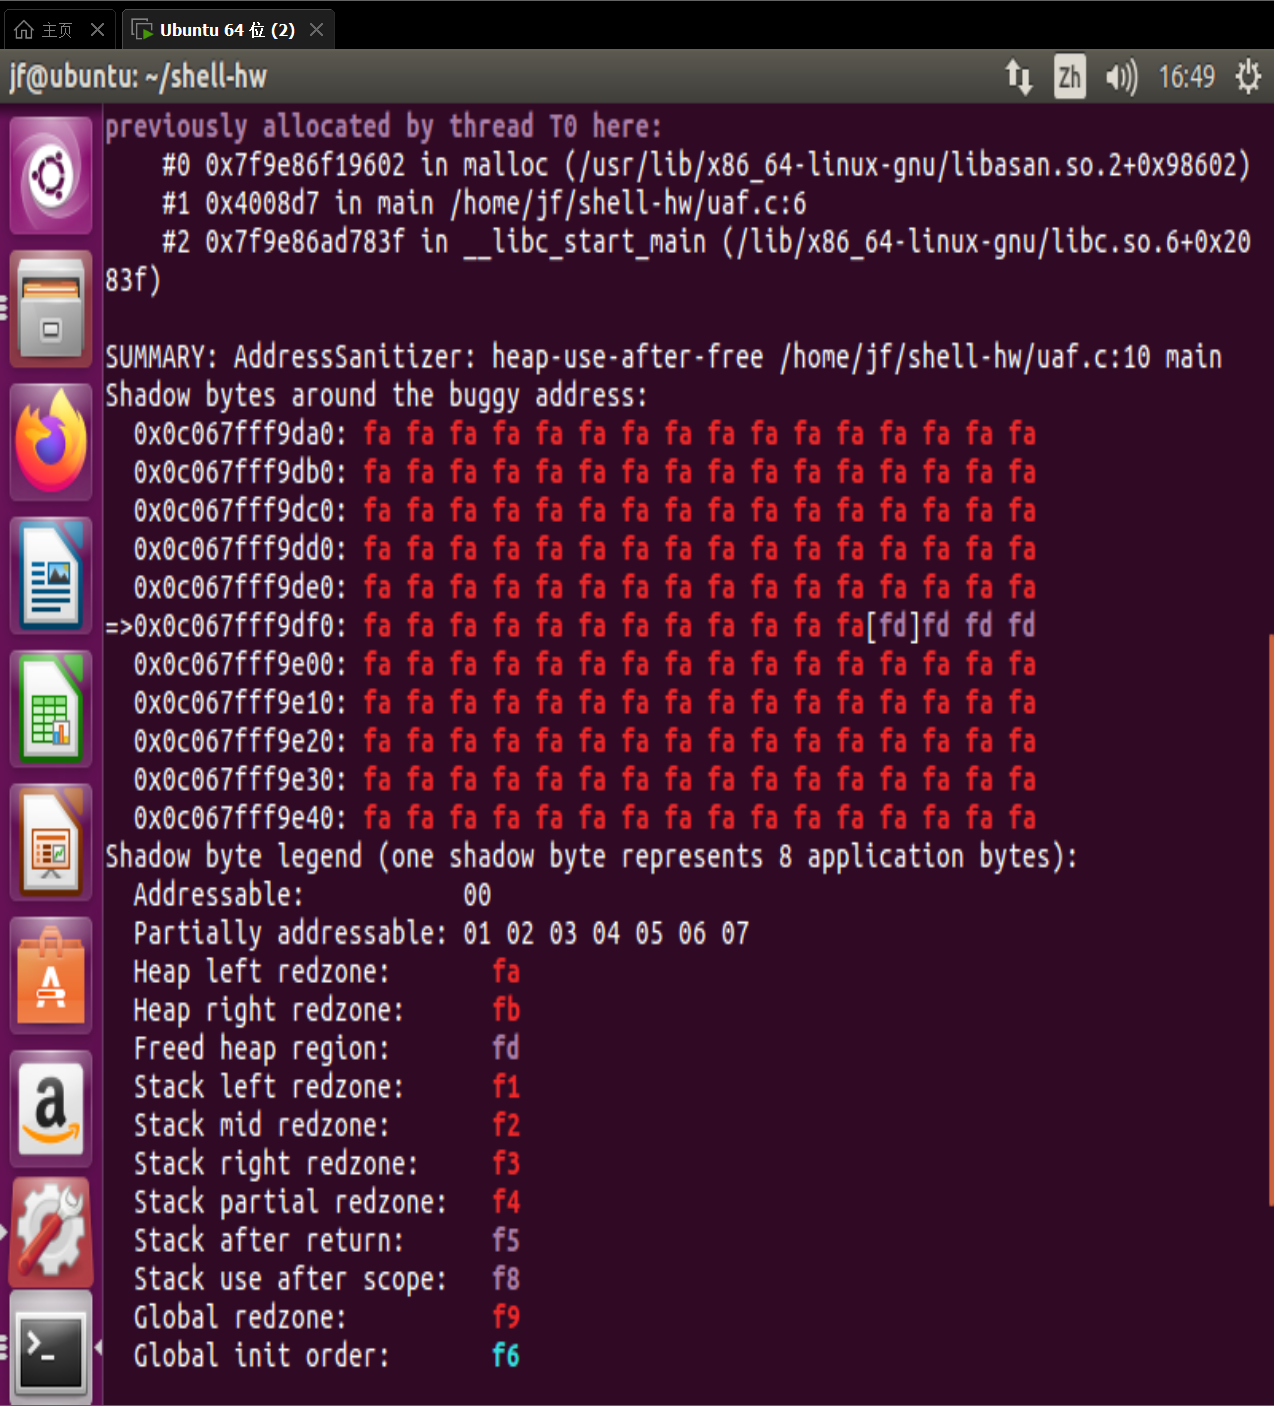
\includegraphics[width=0.9\textwidth]{asan_error.png}
    \caption{ASan 错误报告：heap-use-after-free，指出出错、释放、分配的位置}
    \label{fig:asan_error}
\end{figure}

\begin{figure}[H]
    \centering
    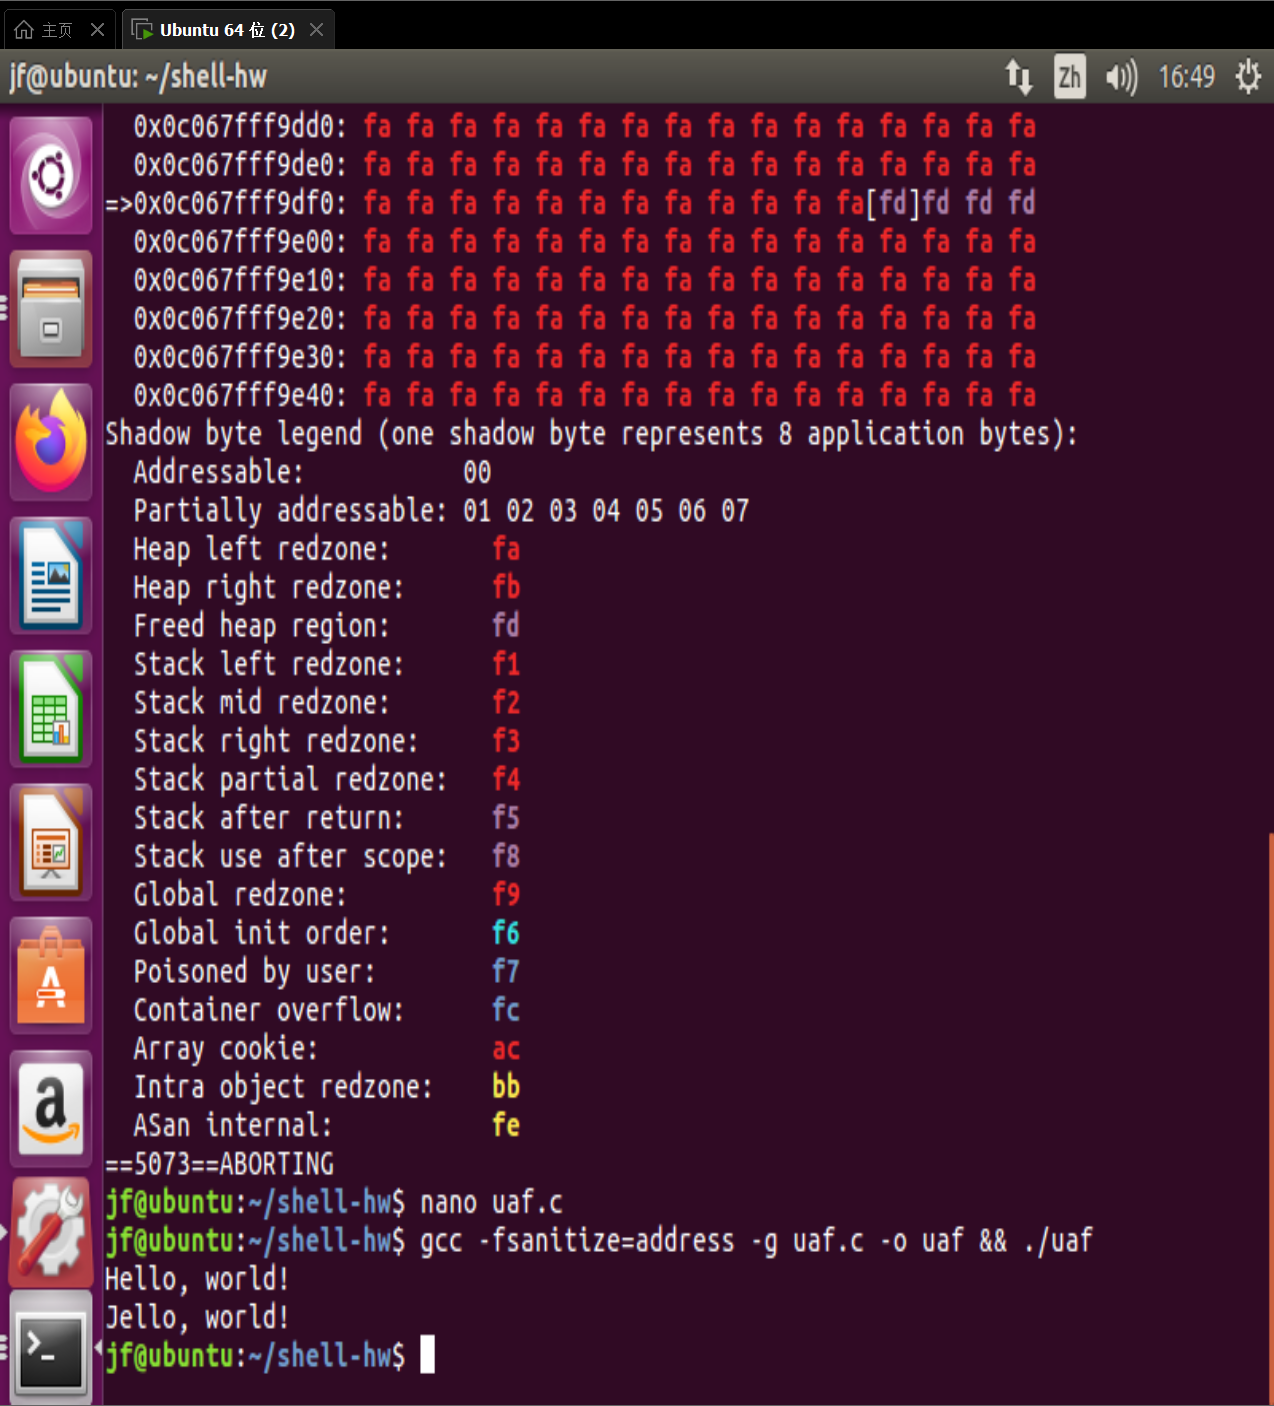
\includegraphics[width=0.9\textwidth]{asan_fixed.png}
    \caption{Shadow 字节布局与修复说明（ABORTING 后程序继续运行输出）}
    \label{fig:asan_fixed}
\end{figure}

\textbf{修复}：把写操作移到 free 之前，或在 free 后不再访问该指针。最简单的最小修改是把第 9 行的 free(greeting) 移到所有使用之后，避免释放后使用。

\subsubsection*{小结}
普通的 gcc 编译运行"看起来正常"，但用 AddressSanitizer 编译后能精确报告 heap-use-after-free，并给出出错位置（uaf.c:10）、释放位置（uaf.c:9）和分配位置（uaf.c:6），这就是内存调试工具的价值。

% ==================== 练习 8：端口占用 ====================
\subsection{端口占用排查}

\textbf{题目}：A common issue is that a port you want to listen on is already taken by another process. Learn how to discover that process: First execute python -m http.server 4444 to start a minimal web server on port 4444. On a separate terminal run ss -tlnp | grep 4444 to find the process. Terminate it with kill <PID>.

\begin{figure}[H]
    \centering
    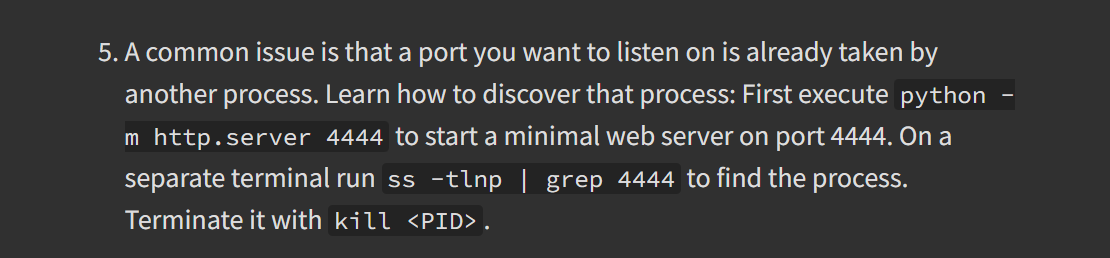
\includegraphics[width=0.9\textwidth]{port_question.png}
    \caption{练习题目要求}
    \label{fig:port_question}
\end{figure}

\subsubsection*{作答过程与运行结果}

\begin{lstlisting}[language=bash, caption={启动服务、查找占用进程、终止}]
$ python3 -m http.server 4444
Serving HTTP on 0.0.0.0 port 4444 ...
$ ss -tlnp | grep 4444
LISTEN 0 5 *:4444  *:*  users:(("python3",pid=7169,fd=3))
$ kill 7169
$ ss -tlnp | grep 4444
$   # 无输出，说明端口已被释放
\end{lstlisting}

\begin{figure}[H]
    \centering
    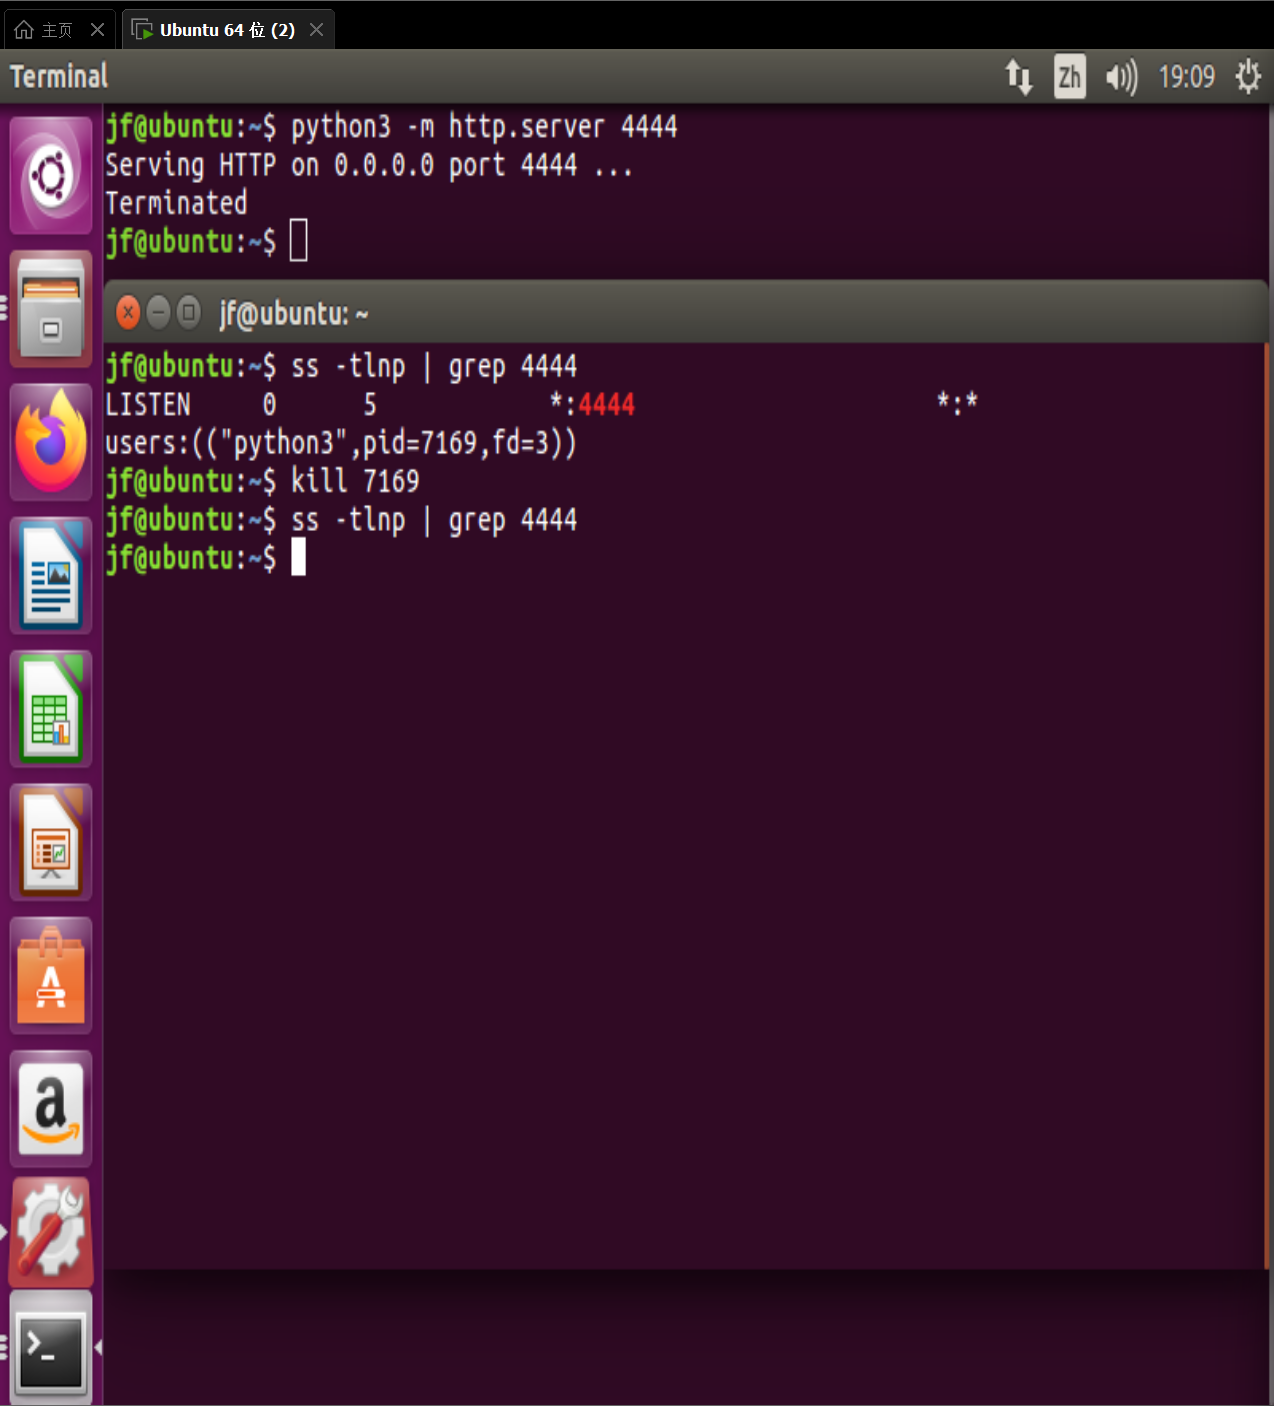
\includegraphics[width=0.9\textwidth]{port_run.png}
    \caption{启动 http.server，ss -tlnp 找到 pid=7169，kill 后端口释放}
    \label{fig:port_run}
\end{figure}

\subsubsection*{小结}
当端口被占用时，用 ss -tlnp 加 grep 端口号即可查到占用进程及其 PID（这里为 python3, pid=7169），再 kill 该 PID 即可释放端口。

% ==================== 练习 9：SSH 密钥 ====================
\subsection{SSH 密钥生成}

\textbf{题目}：进入 ~/.ssh/，检查你是否已经有一对 SSH 密钥。如果没有，就用 ssh-keygen -a 100 -t ed25519 生成一对。建议给密钥设置密码，并配合 ssh-agent 使用。

\begin{figure}[H]
    \centering
    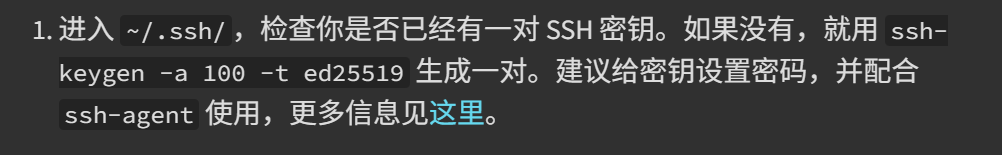
\includegraphics[width=0.9\textwidth]{sshkey_question.png}
    \caption{练习题目要求}
    \label{fig:sshkey_question}
\end{figure}

\subsubsection*{作答过程与运行结果}

\begin{lstlisting}[language=bash, caption={检查已有密钥并重新生成}]
$ ls -la ~/.ssh/
drwx------ 2 jf jf 4096 Aug 24 07:12 .
-rw------- 1 jf jf 411 Aug 24 06:43 id_ed25519
-rw-r--r-- 1 jf jf 97  Aug 24 06:43 id_ed25519.pub
-rw------- 1 jf jf 3247 Aug 24 07:12 id_rsa
-rw-r--r-- 1 jf jf 735  Aug 24 07:12 id_rsa.pub
-rw-r--r-- 1 jf jf 444  Aug 24 07:09 known_hosts
$ ssh-keygen -a 100 -t ed25519
Generating public/private ed25519 key pair.
Enter file in which to save the key (/home/jf/.ssh/id_ed25519):
/home/jf/.ssh/id_ed25519 already exists.
Overwrite (y/n)? y
Enter passphrase (empty for no passphrase):
Enter same passphrase again:
Your identification has been saved in /home/jf/.ssh/id_ed25519.
Your public key has been saved in /home/jf/.ssh/id_ed25519.pub.
The key fingerprint is:
SHA256:W4U10erkhi8qaxW4gz2wNXmXIqku1jnNuE39Di7Wm5w jf@ubuntu
\end{lstlisting}

\begin{figure}[H]
    \centering
    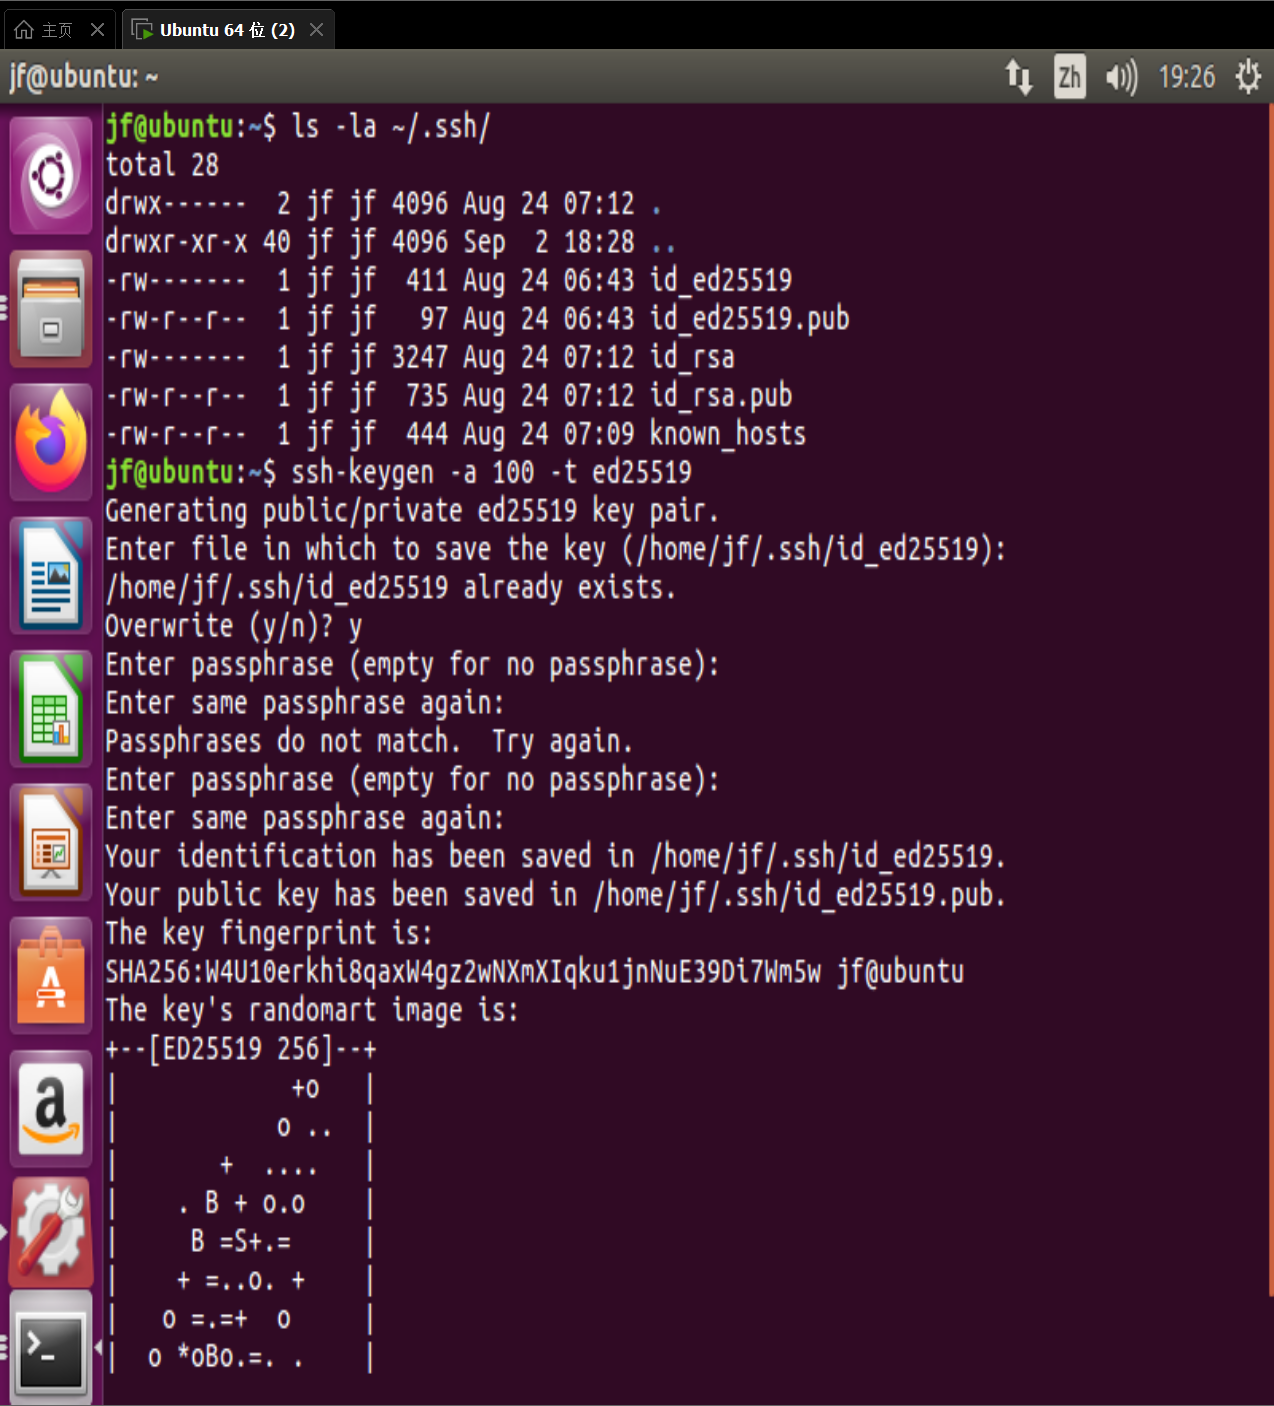
\includegraphics[width=0.9\textwidth]{sshkey_run.png}
    \caption{检查 ~/.ssh 下已有密钥，用 ssh-keygen 重新生成 ed25519 密钥对}
    \label{fig:sshkey_run}
\end{figure}

\begin{figure}[H]
    \centering
    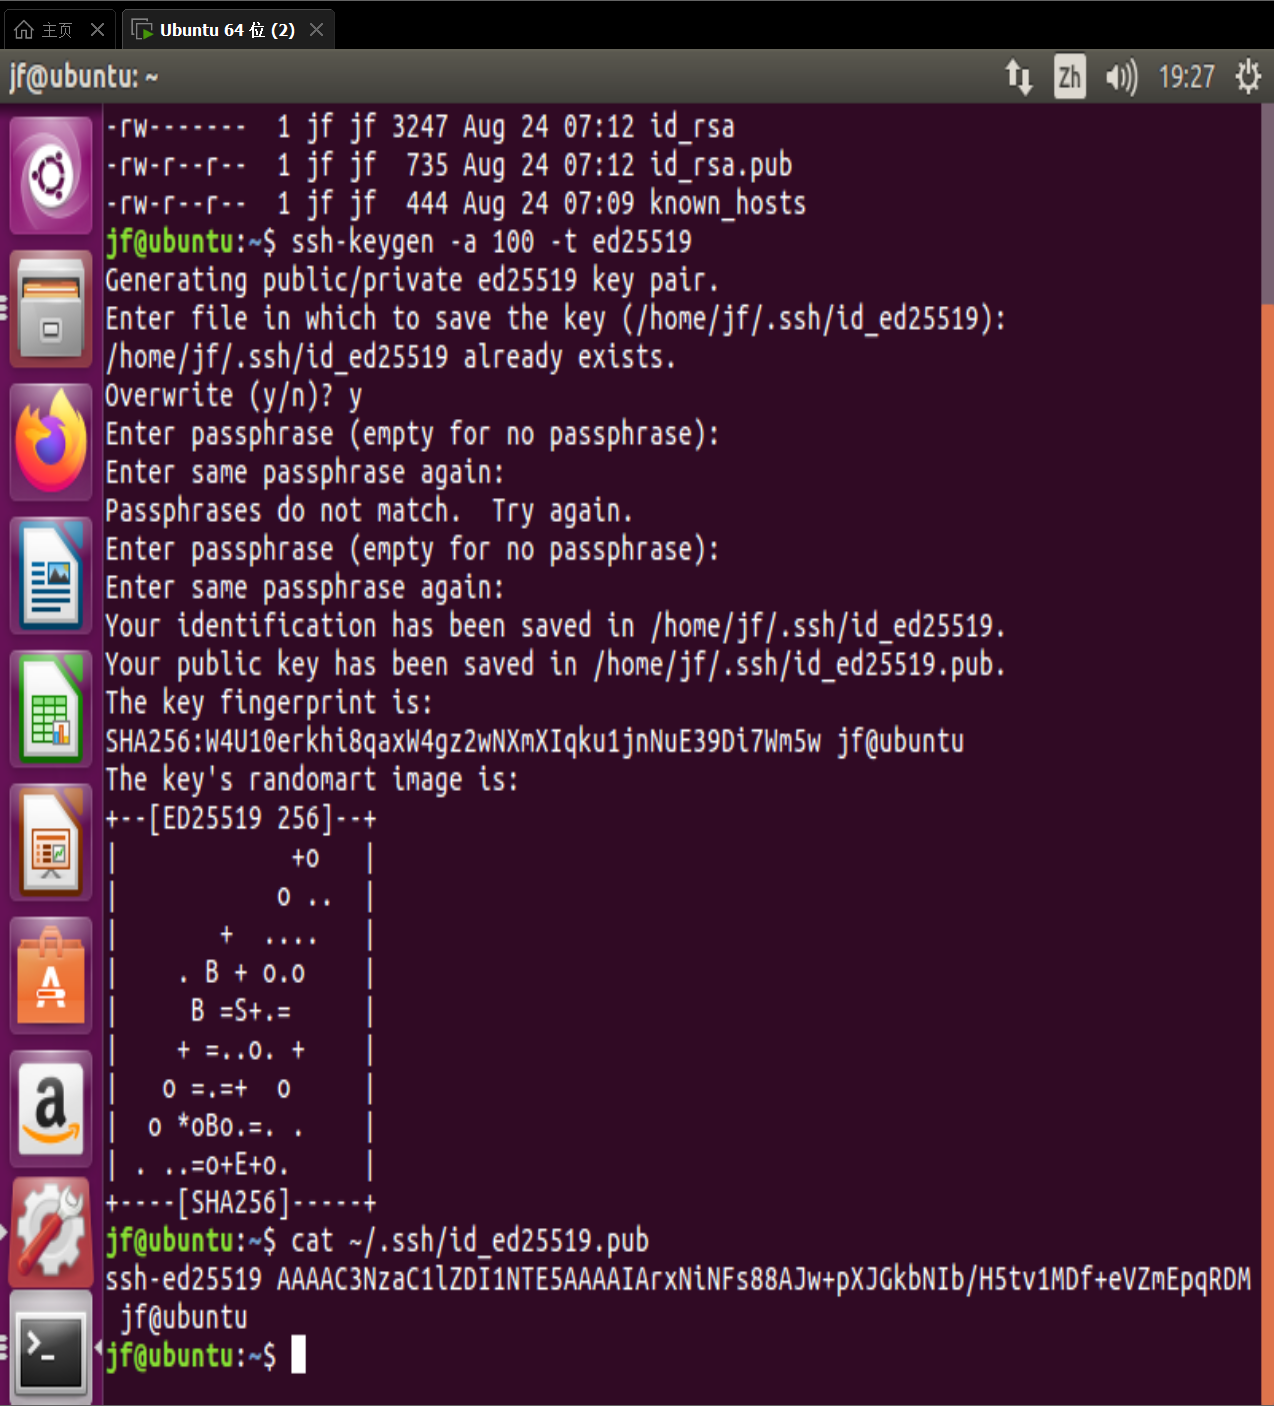
\includegraphics[width=0.9\textwidth]{sshkey_pub.png}
    \caption{密钥生成完成，cat 查看公钥内容}
    \label{fig:sshkey_pub}
\end{figure}

\subsubsection*{小结}
通过 ls -la ~/.ssh 检查密钥，用 ssh-keygen -a 100 -t ed25519 生成更安全的 ed25519 密钥对（并设置 passphrase）；公钥 id\_ed25519.pub 可添加到远程主机以实现免密登录。

% ==================== 练习 10：SSH 配置 ====================
\subsection{SSH 配置文件}

\textbf{题目}：编辑 .ssh/config，加入下面这样的配置项：Host vm、User username、HostName ip、IdentityFile ~/.ssh/id\_ed25519、LocalForward 9999 localhost:8888。

\begin{figure}[H]
    \centering
    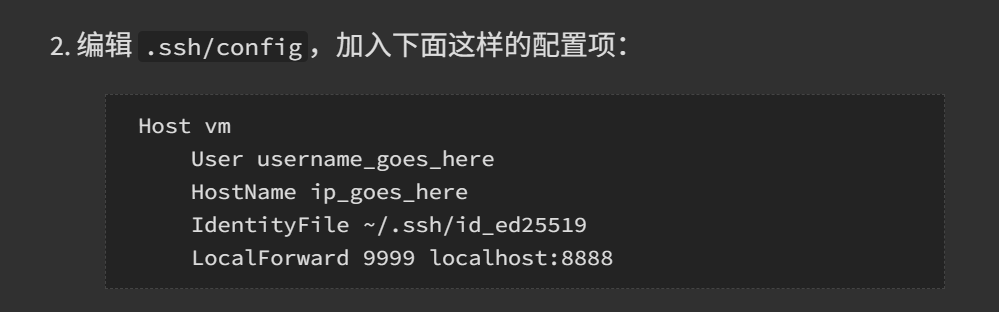
\includegraphics[width=0.9\textwidth]{sshcfg_question.png}
    \caption{练习题目要求}
    \label{fig:sshcfg_question}
\end{figure}

\subsubsection*{作答过程与运行结果}

\begin{lstlisting}[language=bash, caption={~/.ssh/config 配置内容}]
Host vm
    User jf
    HostName 192.168.1.100
    IdentityFile ~/.ssh/id_ed25519
    LocalForward 9999 localhost:8888
\end{lstlisting}

\begin{figure}[H]
    \centering
    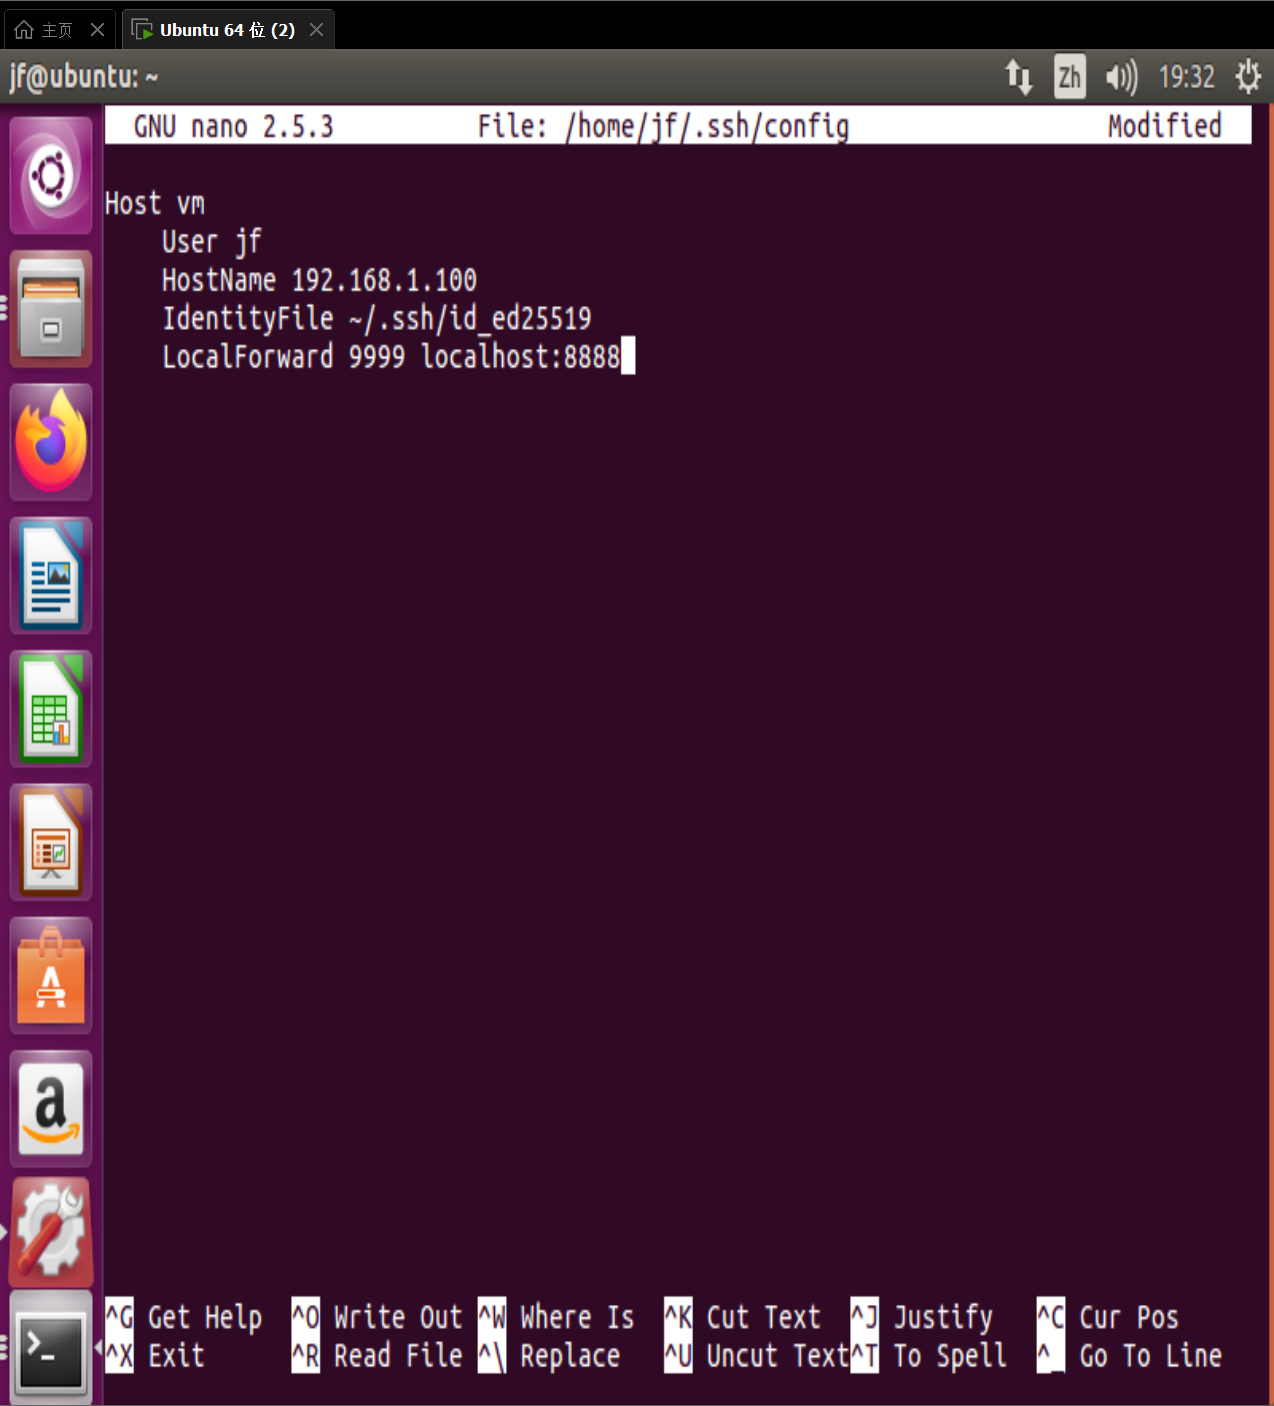
\includegraphics[width=0.9\textwidth]{sshcfg_code.png}
    \caption{nano 中编辑 ~/.ssh/config（Host vm 配置项）}
    \label{fig:sshcfg_code}
\end{figure}

\begin{lstlisting}[language=bash, caption={设置权限并验证配置}]
$ chmod 600 ~/.ssh/config
$ ssh -G vm | head -15
user jf
hostname 192.168.1.100
port 22
identityfile ~/.ssh/id_ed25519
...
\end{lstlisting}

\begin{figure}[H]
    \centering
    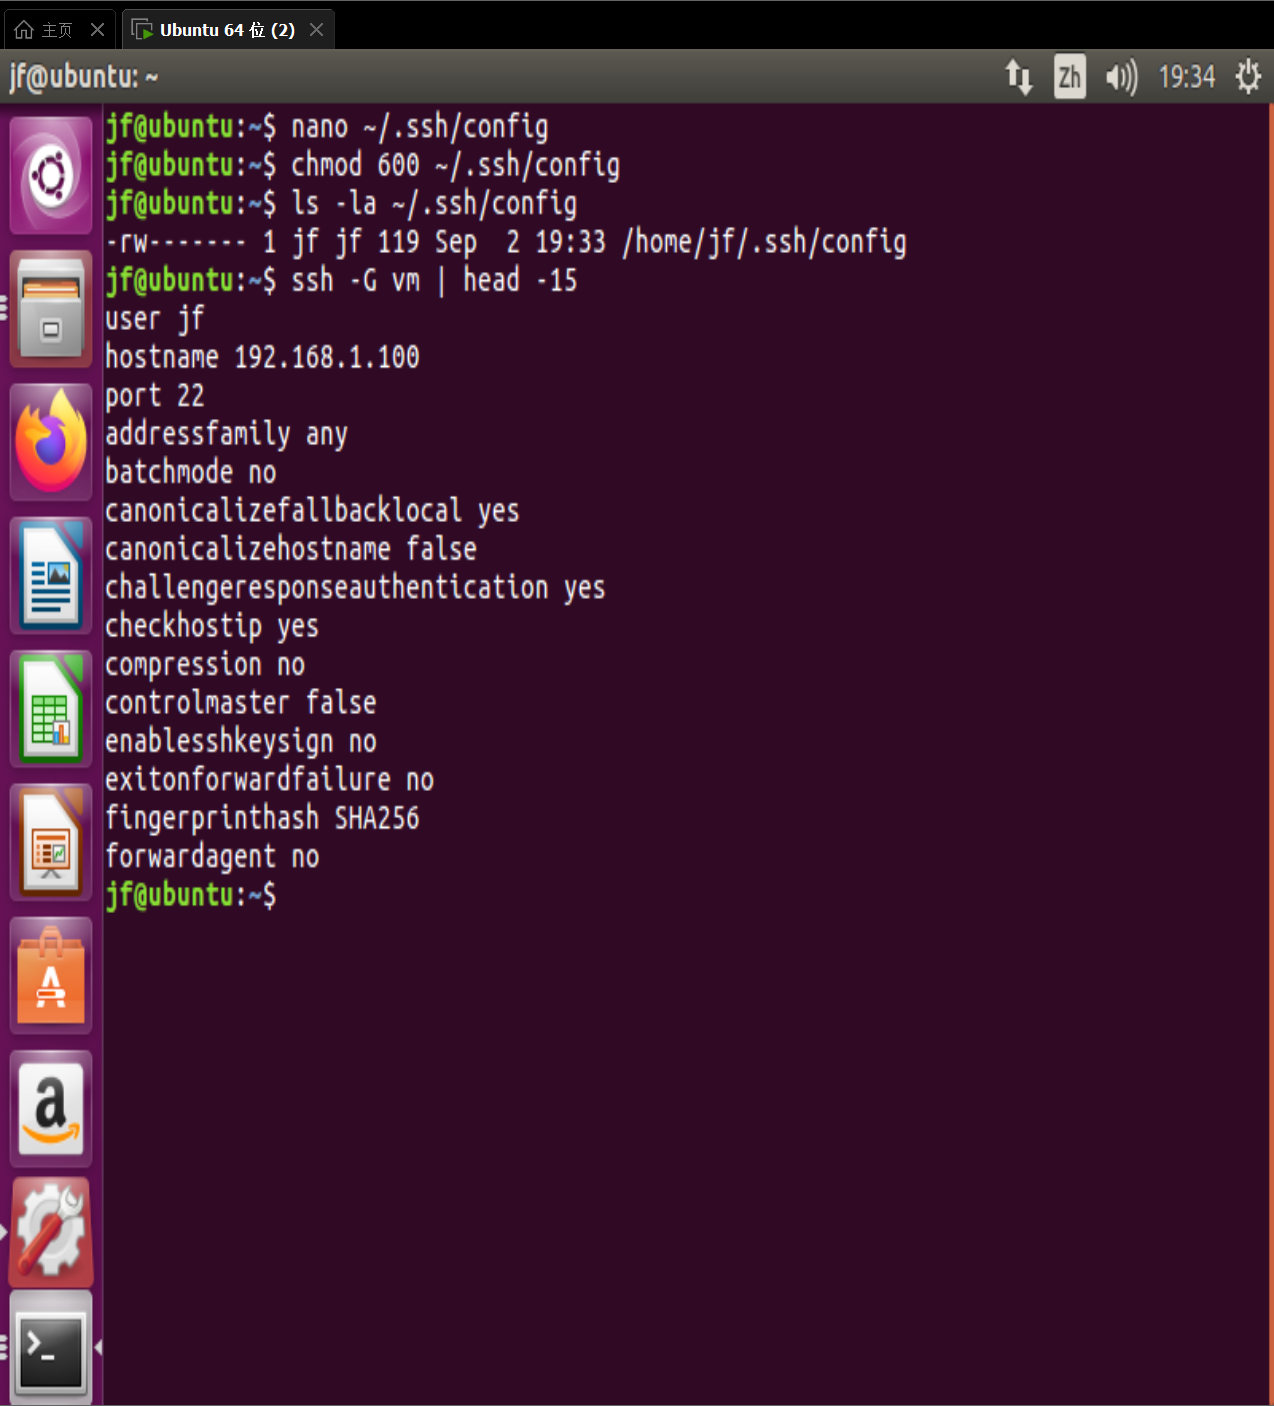
\includegraphics[width=0.9\textwidth]{sshcfg_run.png}
    \caption{chmod 600 设置权限，ssh -G vm 验证配置生效}
    \label{fig:sshcfg_run}
\end{figure}

\subsubsection*{小结}
在 ~/.ssh/config 中定义 Host vm 后，直接 ssh vm 即可按配置连接（用户、主机、密钥、本地端口转发 9999→localhost:8888）；chmod 600 保证私钥配置文件的权限安全。

% ==================== 练习 11：Vim ====================
\subsection{Vim 编辑器}

\textbf{题目}：安装并使用 Vim 完成练习：用 vim 打开 vimchallenge.txt，将每行单词的首字母大写；并完成一道 VimGolf 挑战。

\begin{figure}[H]
    \centering
    
\includegraphics[width=0.9\textwidth]{vim_question.png}
    \caption{练习题目要求（完成一道 VimGolf 挑战）}
    \label{fig:vim_question}
\end{figure}

\subsubsection*{作答过程与运行结果}

系统未安装 vim，先用 apt 安装并查看版本：

\begin{lstlisting}[language=bash, caption={安装 vim 并确认版本}]
$ vim vimchallenge.txt
The program 'vim' can be found in the following packages: ...
$ sudo apt install vim -y
Reading package lists... Done
...
$ vim --version
VIM - Vi IMproved 7.4 ...
\end{lstlisting}

\begin{figure}[H]
    \centering
    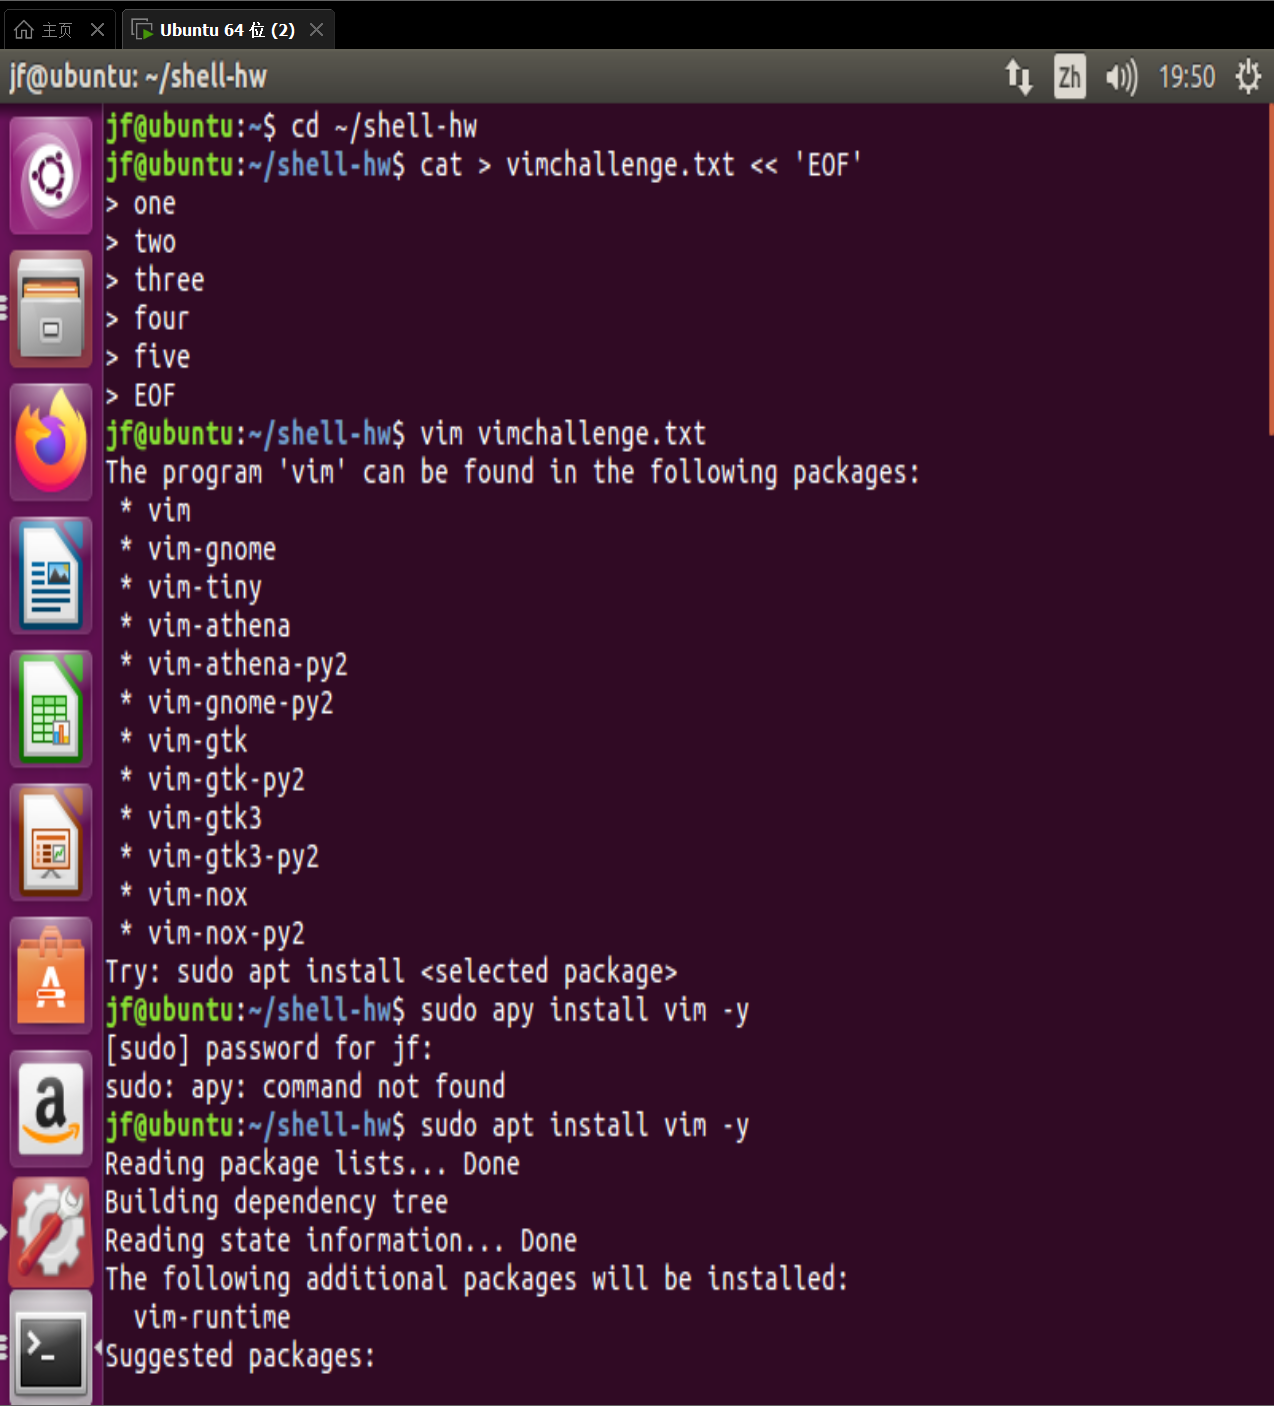
\includegraphics[width=0.9\textwidth]{vim_install.png}
    \caption{创建 vimchallenge.txt，vim 未安装，用 sudo apt install vim -y 安装}
    \label{fig:vim_install}
\end{figure}

\begin{figure}[H]
    \centering
    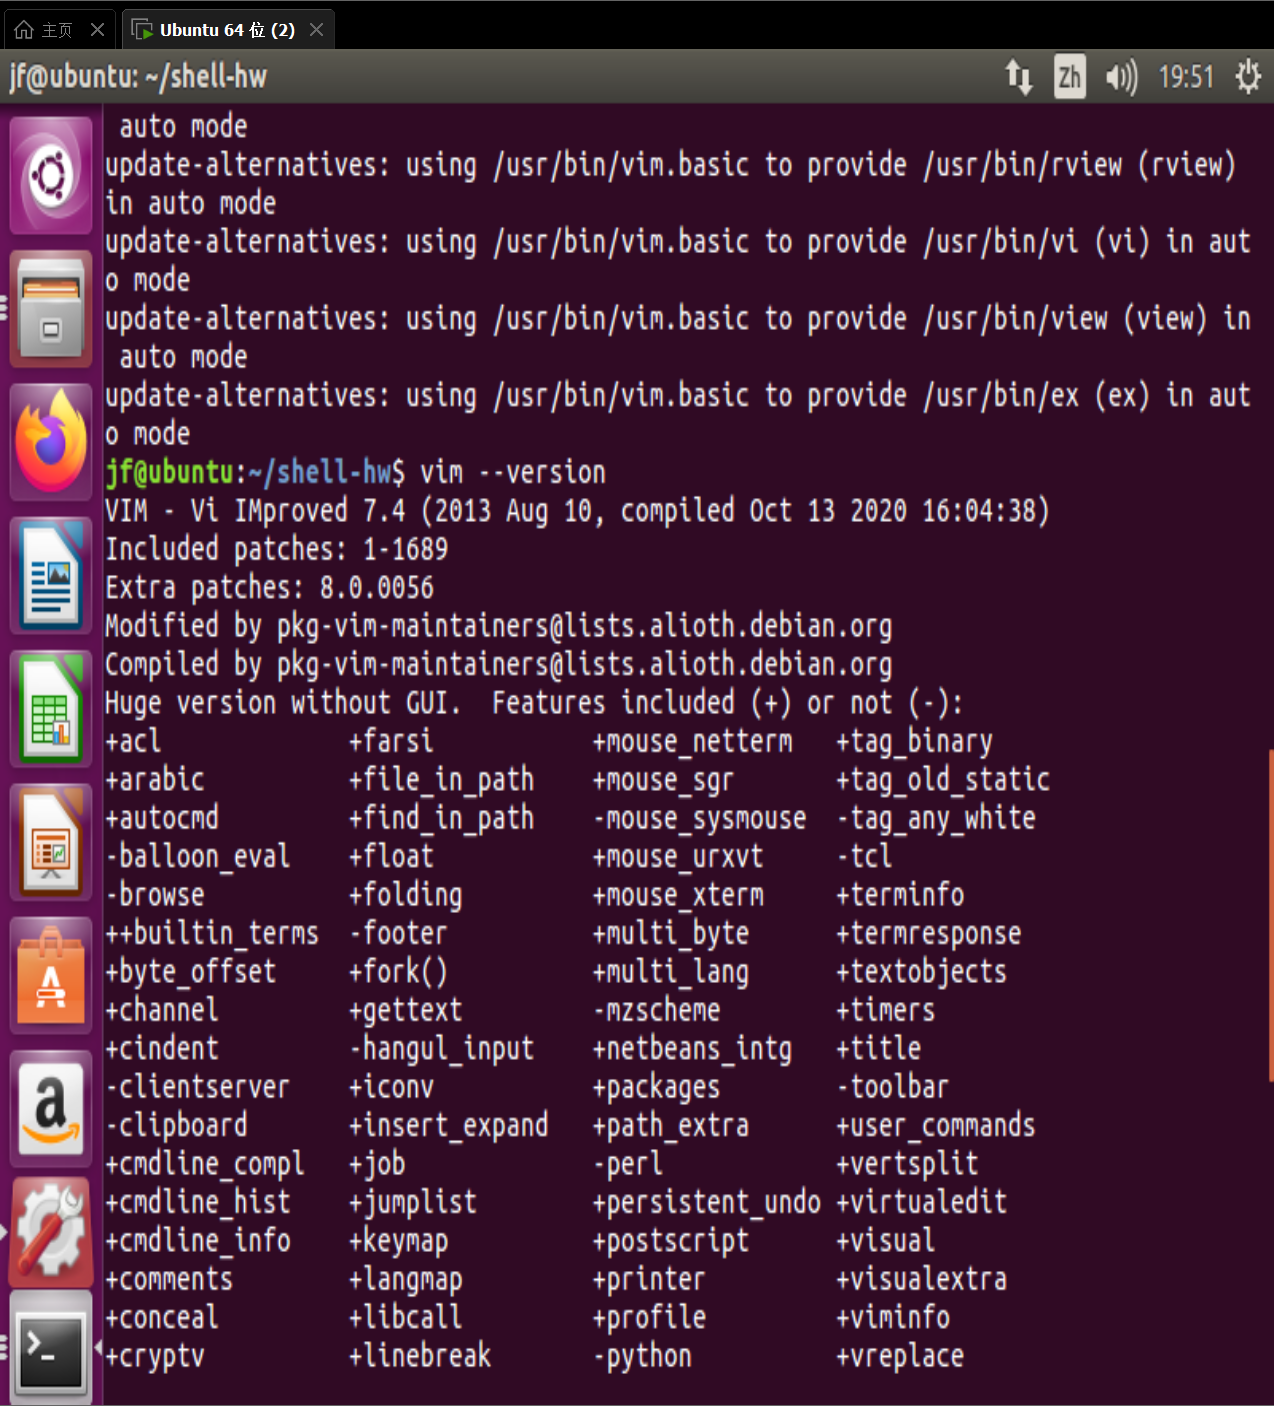
\includegraphics[width=0.9\textwidth]{vim_version.png}
    \caption{vim --version 确认安装完成}
    \label{fig:vim_version}
\end{figure}

\begin{figure}[H]
    \centering
    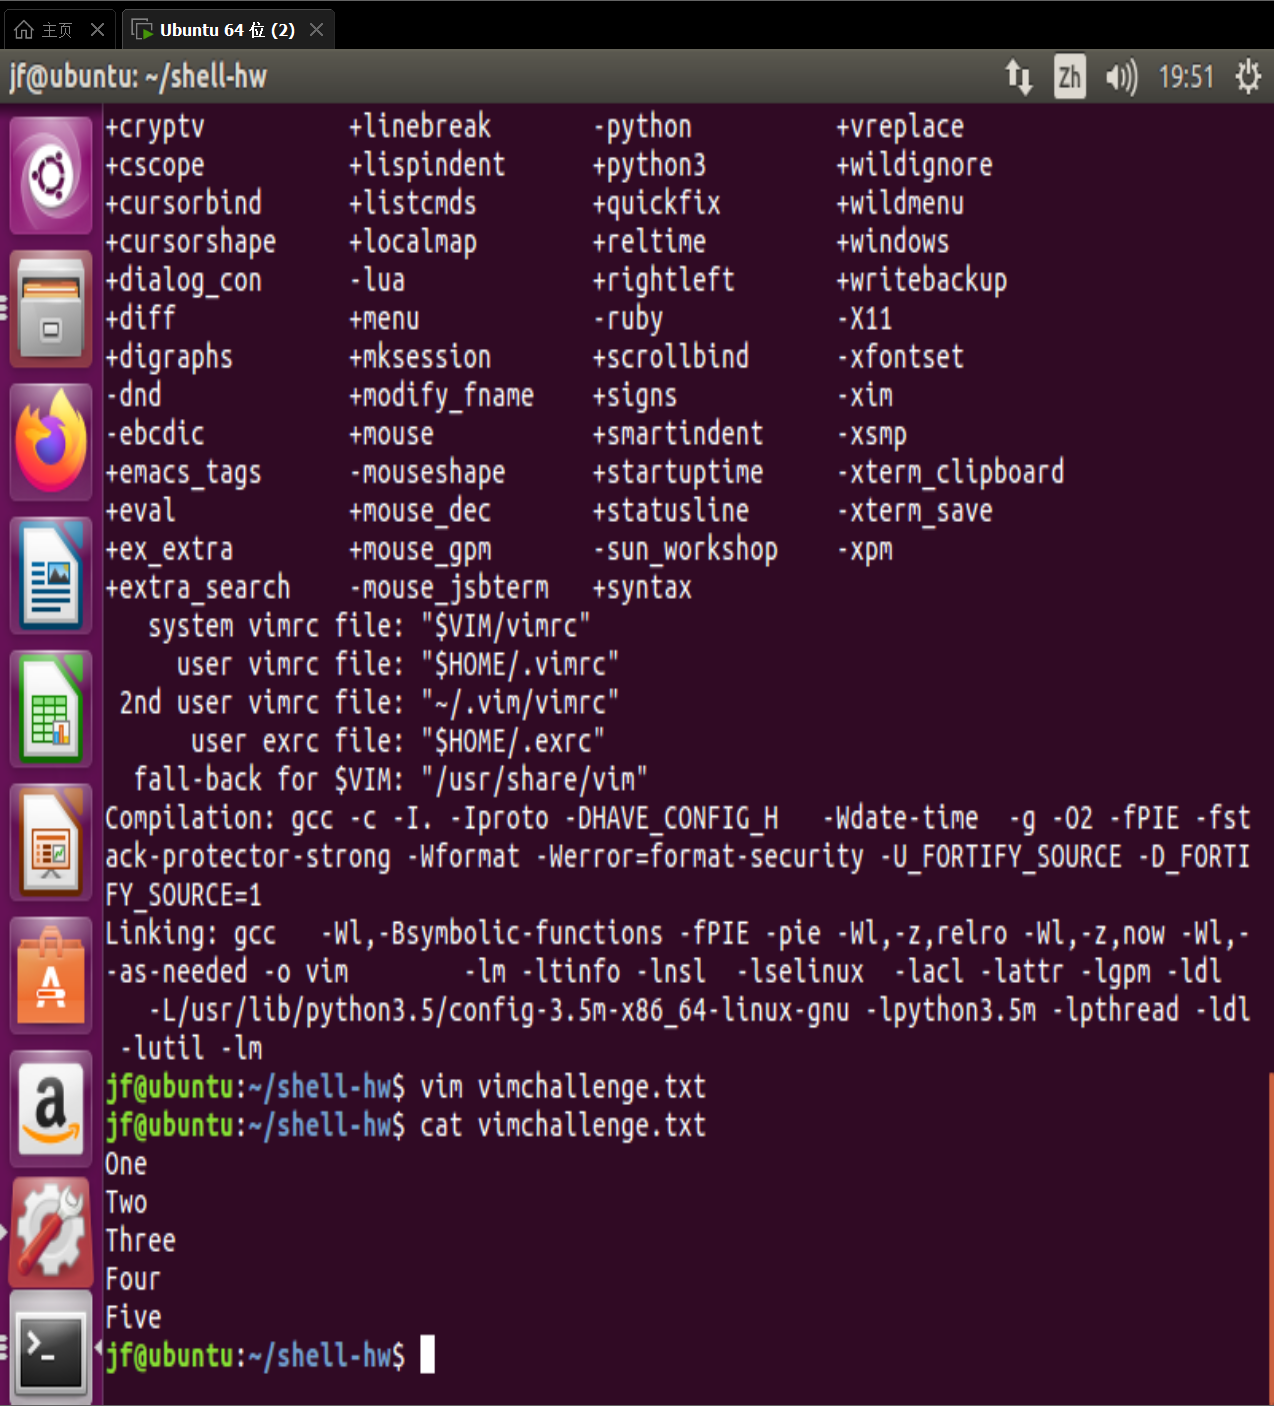
\includegraphics[width=0.9\textwidth]{vim_version2.png}
    \caption{vim 版本详情、编译参数与配置文件路径}
    \label{fig:vim_version2}
\end{figure}

在 Vim 中使用替换命令把每行首字母改为大写（对应 VimGolf 挑战）：用命令模式输入 \texttt{:1,5s/\^{}./\textbackslash{}u\&/g}，把第 1 到 5 行每行的第一个字符大写：

\begin{lstlisting}[language=bash, caption={Vim 中首字母大写替换}]
# 文件内容 one/two/three/four/five
:1,5s/^./\u&/g
# 执行后：
One
Two
Three
Four
Five
\end{lstlisting}

\begin{figure}[H]
    \centering
    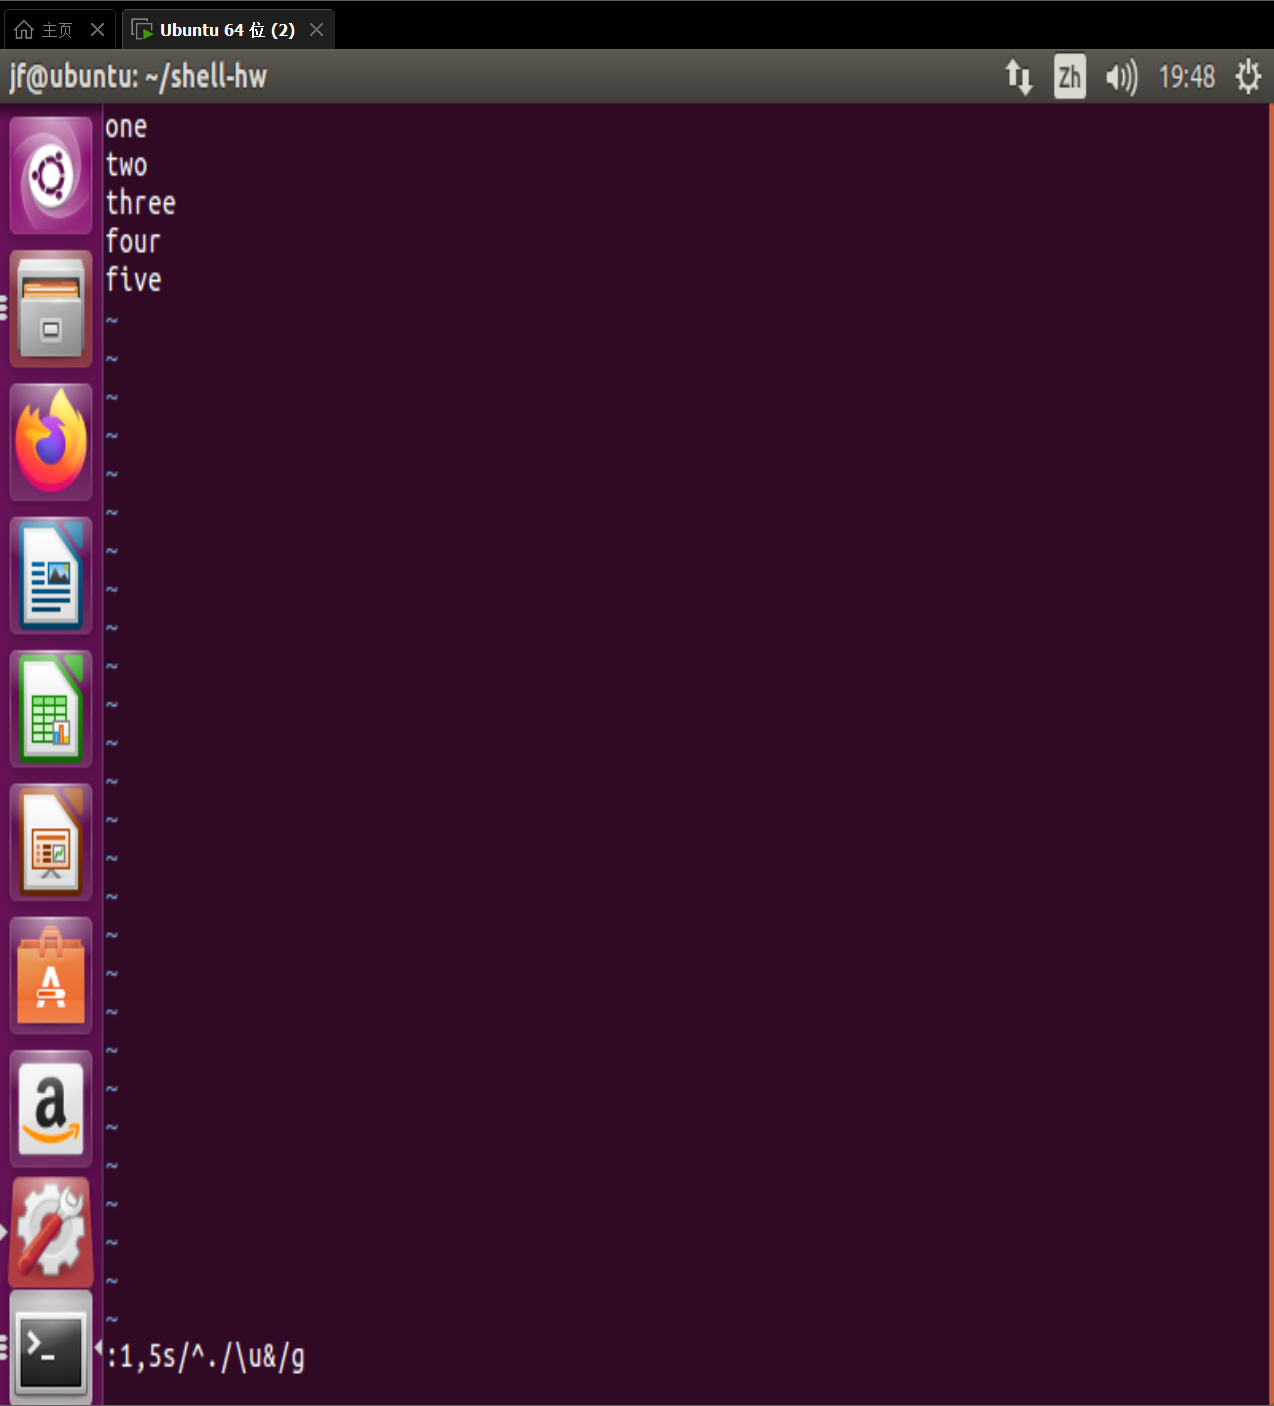
\includegraphics[width=0.9\textwidth]{vim_edit.png}
    \caption{Vim 命令模式中输入 :1,5s/^./\u&/g}
    \label{fig:vim_edit}
\end{figure}

\begin{figure}[H]
    \centering
    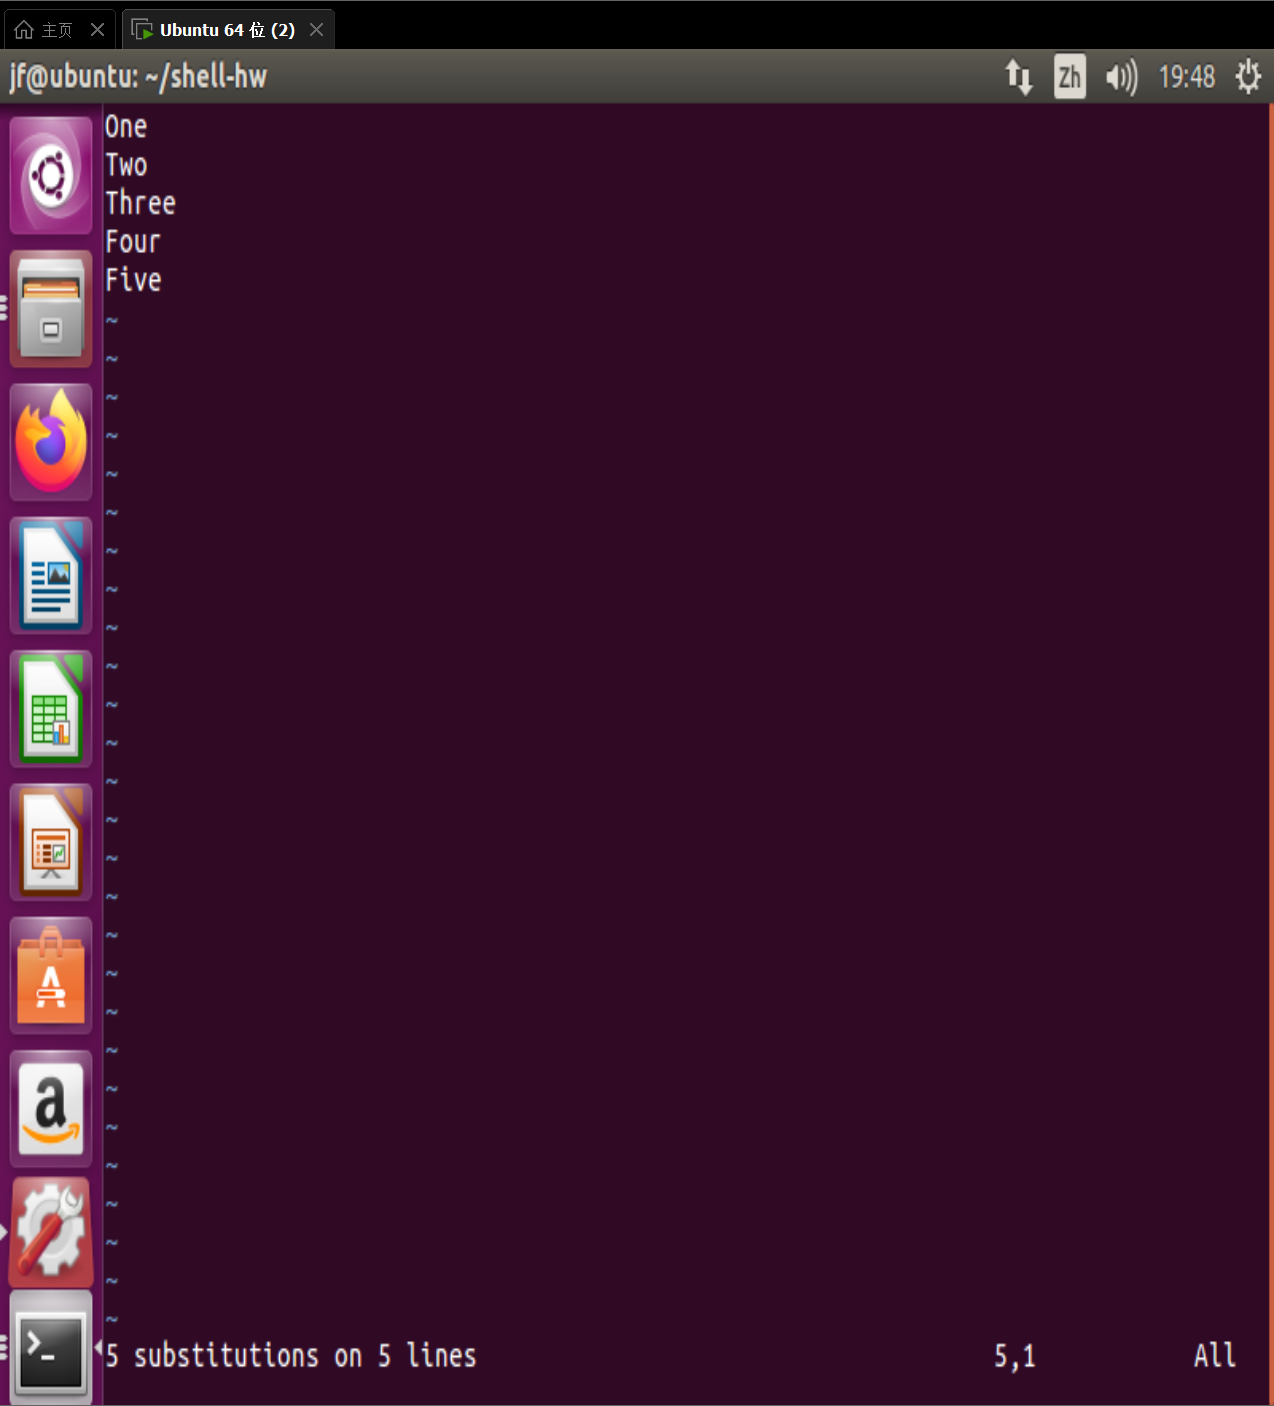
\includegraphics[width=0.9\textwidth]{vim_result.png}
    \caption{替换完成：5 substitutions on 5 lines，首字母全部大写}
    \label{fig:vim_result}
\end{figure}

\subsubsection*{小结}
Vim 中 :1,5s/^./\u&/g 用正则把第 1~5 行行首字符替换为其大写形式（\textbackslash{}u 表示大写，\& 表示匹配到的内容），5 行全部替换成功。整个练习体验了 vim 的安装、版本查看与命令模式下的批量替换操作。

% ----------------------------------------------------------------------------
% 3. 代码仓库与提交记录
% ----------------------------------------------------------------------------
\section{代码仓库与提交记录}

按照课程要求，本次实验的练习、代码等已上传到个人 GitHub 账号，并保留分步 commit 记录。

\subsection{仓库链接}
\begin{itemize}
    \item 仓库地址：\url{https://github.com/GJF080117/jf}
    \item 提交者：GJF080117
\end{itemize}

\subsection{commit 记录截图}

\begin{figure}[H]
    \centering
    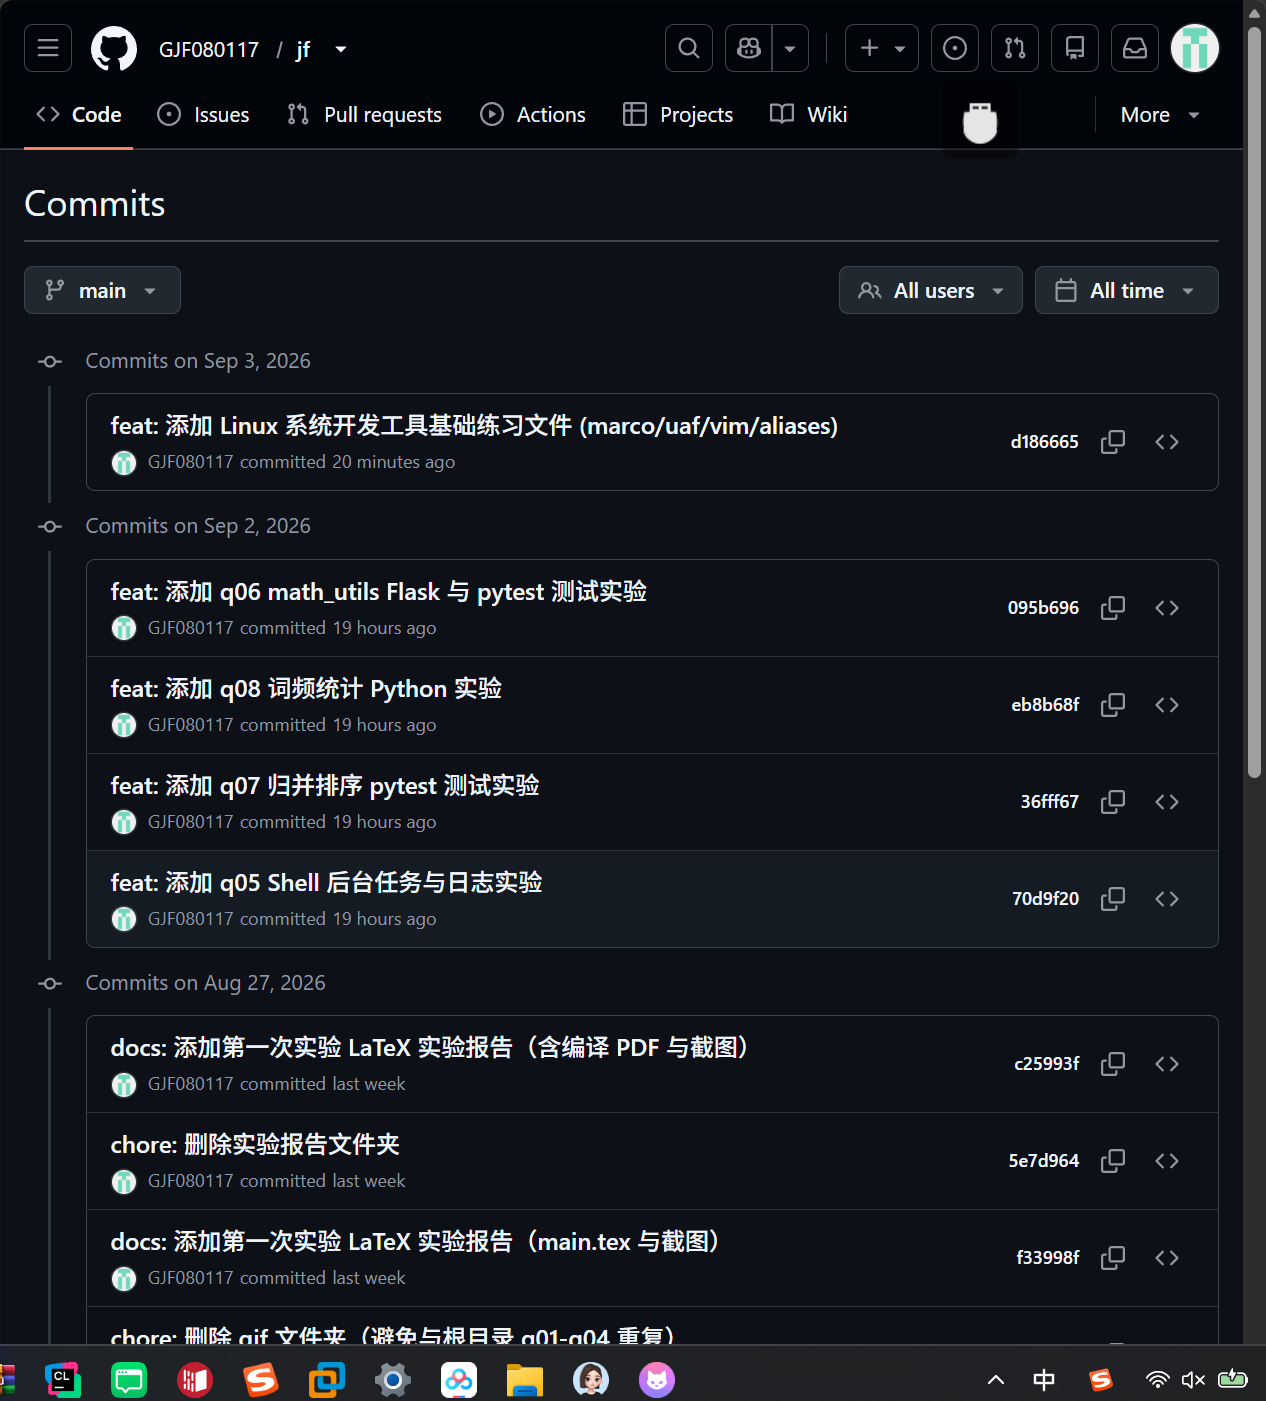
\includegraphics[width=0.9\textwidth]{commit1.png}
    \caption{仓库提交记录（9 月 3 日：marco/uaf/vim/aliases 练习；9 月 2 日：q05--q08 实验）}
    \label{fig:commit1}
\end{figure}

\begin{figure}[H]
    \centering
    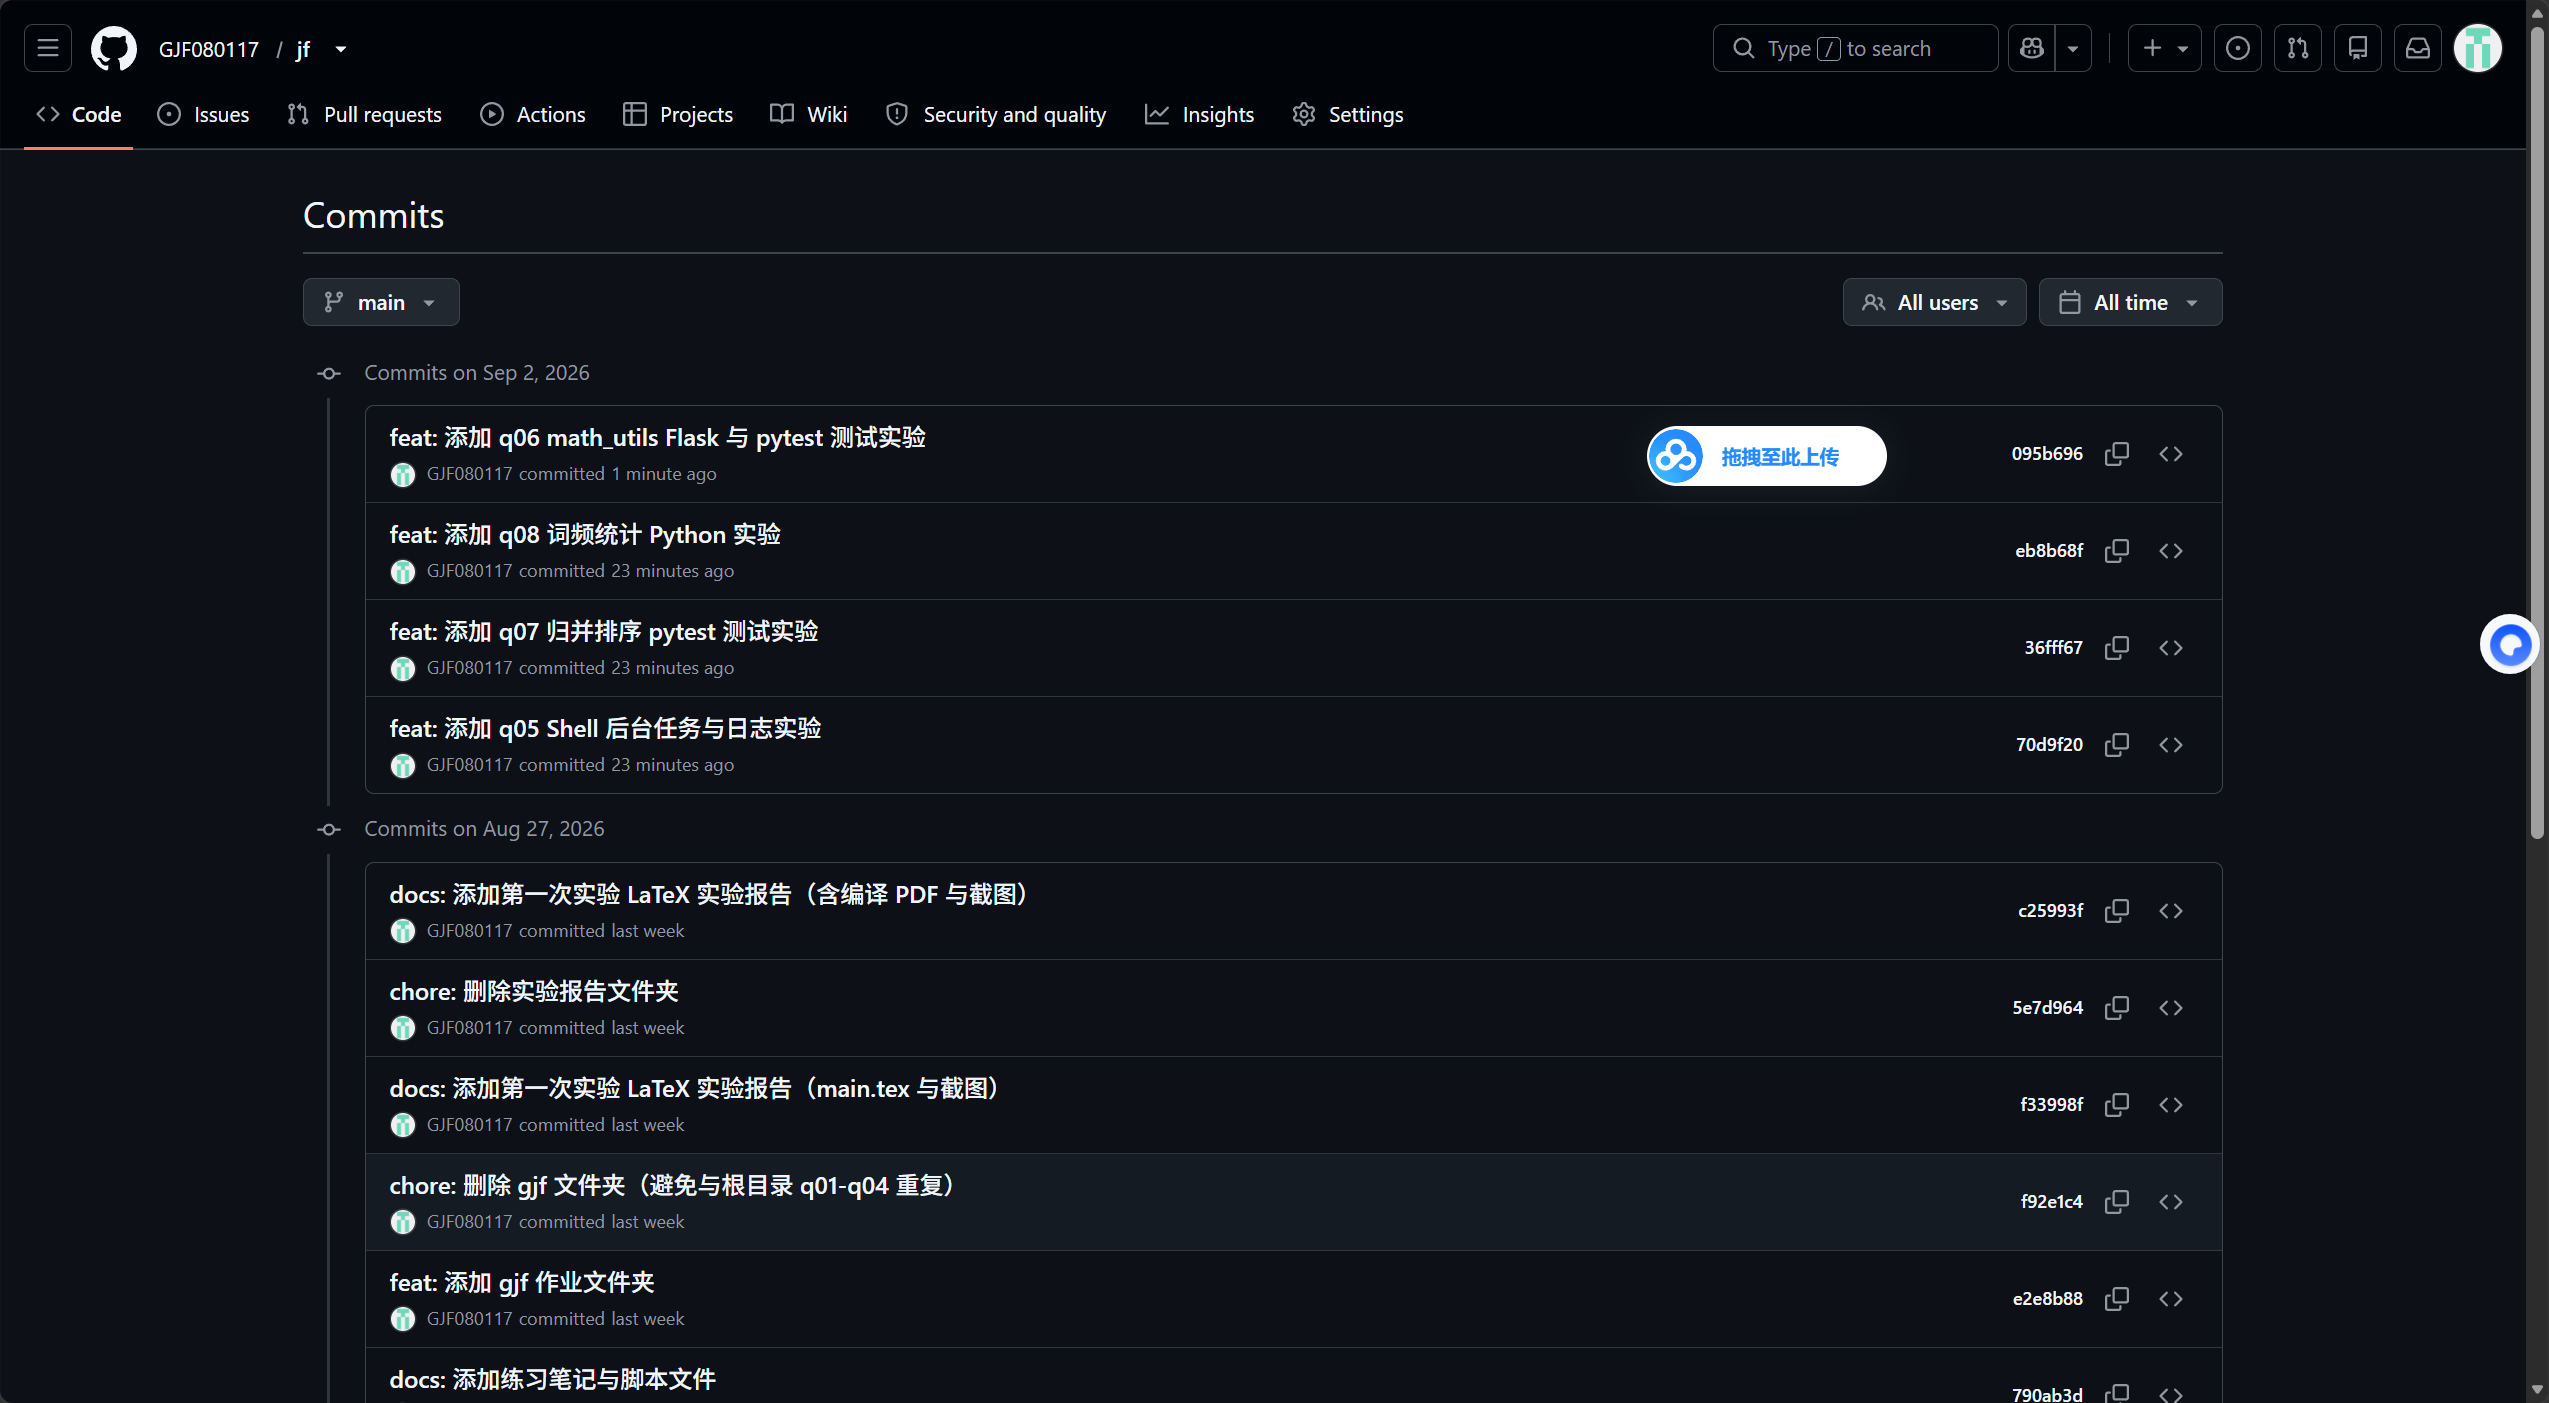
\includegraphics[width=0.9\textwidth]{commit2.png}
    \caption{提交记录（按"练习文件—实验代码—实验报告"分步提交）}
    \label{fig:commit2}
\end{figure}

\subsection{提交说明}
本次提交采用分主题、分步提交的策略，例如：先提交 q05 后台任务实验，再依次提交 q07 归并排序调试、q08 词频统计实验，最后提交第二次实验的 Linux 开发工具练习文件（marco/uaf/vim/aliases），每次提交均附有清晰的 commit message，避免单次全量提交。

% ============================================================================
% 声明
% ============================================================================
\vspace{2em}
\begin{flushright}
    \begin{minipage}{0.55\textwidth}
        \noindent 本人声明：本报告内容为本人独立完成，代码与练习均来自本人实际操作。\\
        \vspace{0.8em}
        \hfill 签名：\underline{\hspace{4em}} \\
        \hfill 日期：\underline{\hspace{4em}}
    \end{minipage}
\end{flushright}
\end{document}
